% lathese.tex
% author: Claudia Esteves (but it is inspired from many many documents on the internet)
% 
% -------------------------------------------------------------
% additional files:
% 		titlepage.tex			Title and School Information
% 		abstract_en.tex			Abstract
%		acknowledgements.tex	Acknowledgement
% 		intro.tex				Introduction
%		statusquo.tex			State of the Art
%		representation.tex		Models and notations
%		eugene.tex	
%		buran.tex
%		hrp2.tex
%		conclusions.tex
%		lathese.bib		
% ---------------------------------------------------------------

\documentclass[final]{./styles/lathese}

\TheTitle{Vision-Based Locomotion for Humanoid Robots}
\TheAuthor{Mauricio Josafat Garc\'ia V\'azquez}
\TheDate{23 de Noviembre de 2013}
\TheAdvisor{Jean-Bernard Hayet}
\TheGroup{}


% Figures 
\usepackage{floatflt}
\usepackage{graphicx}
\usepackage{subfigure}
\usepackage{rotating}

%algorithms 
\usepackage[boxed,algochapter,algoruled,lined]{./styles/algorithm2e}

\usepackage[small,normal,bf,sf]{caption}
\renewcommand{\captionfont}{\small}
\usepackage{import}

% Math fonts
\usepackage{amsmath,amsfonts,amssymb}
\usepackage{./styles/manfnt}

\hyphenation{ in-betweens pa-ra-me-ters}
\hyphenpenalty= 10000
\tolerance=1000
\interfootnotelinepenalty=10000

%\bibliographystyle{./styles/acmtrans}
%\usepackage[colorlinks=true]{hyperref}
%\usepackage[]{hyperref}
\usepackage[square]{natbib}
\bibliographystyle{plainnat}

% Force to include the key in the bibliography list
\makeatletter
\def\@lbibitem[#1]#2{%
\if\relax\@extra@b@citeb\relax\else
\@ifundefined{br@#2\@extra@b@citeb}{}{%
\@namedef{br@#2}{\@nameuse{br@#2\@extra@b@citeb}}}\fi
\@ifundefined{b@#2\@extra@b@citeb}{\def\NAT@num{}}{\NAT@parse{#2}}%
\item[\hfil\hyper@natanchorstart{#2\@extra@b@citeb}\citep{#2}%
\hyper@natanchorend]%
\NAT@ifcmd#1(@)(@)\@nil{#2}}
\makeatother

%\usepackage[colorlinks=true, citecolor=blue, linkcolor=blue, urlcolor=blue]{hyperref}
\newcommand\transpose{\top}
\usepackage{multirow}
\usepackage[]{geometry}
\usepackage{pdfpages}
\usepackage{afterpage}

\newcommand\blankpage{%
    \null
    \thispagestyle{empty}%
    \addtocounter{page}{-1}%
    \newpage}

\begin{document}
 
\newgeometry{top=35mm,bottom=30mm,right=25mm,left=25mm}

\includepdf[pages={1}]{portada.pdf}
%\maketitlepage
\restoregeometry

\afterpage{\blankpage}

%
\abstract{ 
\pagestyle{empty}
\small{
We present an approach to introduce visual information in the walking pattern generator for humanoid robots. We make use of visual servoing with model predictive control (MPC), which is joined to the walking motion generator. Since visual servoing with MPC is a nonlinear optimization problem, we propose a linearization scheme in order to keep it as a Quadratic Program (QP) and introduce it within the pattern generator. However, the trajectories realized by the robot are generated by only minimizing the distance in the image feature space and might create unnecessary motion in the space of the footprints. We worked in solving this problem by making the CoM follow a convenient space of trajectories for which the overall behavior of the robot is better.
}
}


\chapter*{Acknowledgements\markboth{Acknowledgements}{Acknowledgements}}

\thispagestyle{empty}



\afterpage{\blankpage}

\frontmatter

\tableofcontents

\mainmatter

% Introduction
%\begin{savequote}[10cm]
%{\it ``The Three Laws of Robotics: \\
%1: A robot may not injure a human being or, through inaction, allow a human being to come to harm; \\
%2: A robot must obey the orders given it by human beings except where such orders would conflict with the First Law;\\
%3: A robot must protect its own existence as long as such protection does not conflict with the First or Second Law.''}
%\qauthor{Isaac Asimov}
%\end{savequote}

\chapter{Introduction} 
\label{Chap:Introduction}

This thesis was made with the spirit of contributing to the autonomy of humanoid robots; more precisely in the development of behaviors based on computer vision. Even with the tremendous expansion of humanoid robotics in the last years, the link between perception and motion generation is still not well developed. Hundreds of works cover both fields separately. In the perception side, computer vision is up to this day the main technique in humanoid robotics. 

On the robotic side, there is an increasing interest in the development of humanoid robotics. Governments and companies such as Honda, Boston Dynamics and Aldebaran Robotics have spent a lot of money in these fields. As a result, amazing demonstrations in humanoid motion generation have been done recently. However, the interaction with the environment is limited in most of the systems.

%% main text
The design of humanoid robots has been done thinking mainly in human-friendly environments, i.e. unstructured and dynamic environments, where objects move outside the robots control. Therefore, when specific tasks have to be completed, these robots have to be able to perceive and react to environmental changes. Visual sensors can help them to reach this objective, by allowing to build local representations of the robot surroundings, and to adapt their behavior in consequence. Most of the existing humanoid platforms are equipped with video cameras, providing the robots with rich information (geometry, texture, color\dots) without adding so much weight and size, at a rather low cost. Moreover, the use of embedded cameras is attractive because it avoids equipping the environment with additional external sensors. Such an embedding increases greatly the level of autonomy of the robotic platform. However, to interpret the data generated from the camera of a humanoid robot is still problematic, with a huge amount of undergoing work in the computer vision community, as, in general, the image quality in humanoid robots is quite poor: blurring effects or vibrations due to the walk may make visual tasks such as  localization and tracking really challenging. 

Early works on humanoid locomotion have assumed that the robot path is defined before computing the current joint control to realize it. This clearly puts limits on the capacities of reaction when changes occur in the environment. These works generally follow a perception-decision-action scheme, in the sense that a sensor first acquires data on the world and/or the robot state, then, suitable footsteps over a time horizon are decided, and finally the trajectories of the Center of Mass (CoM) and the Center of Pressure (CoP) are computed while respecting the stability constraints and avoiding collision with the environment. Finally, the control of the legs and other joints is computed by inverse kinematics, given the previously computed CoM trajectory, and the sequence of footsteps to follow. This perception-decision-action loop has proven to be fast enough  to realize impressive demonstrations for stair-climbing and obstacle avoidance. Our focus in this thesis will be set only on one of the sub-problems necessary to implement this approach: the generation of footsteps and trajectories of the CoM and CoP. We stress that we will not address here the whole body control.


A general diagram of the workflow in humanoid robots is depicted in Fig.~\ref{Fig:GeneralDiagram}. In general we use computer vision to extract information from the environment (mapping, localization, modeling). With this model, we can plan the motion using rules given by a cognitive process. With this plan, the robot performs the dynamic walking which leads to the whole body motion. Computer vision requires high computational load to extract high level information from the scene; motion generation on the other side, requires fast control loops to be dynamically stable. 

\begin{figure}[h!]
\centering
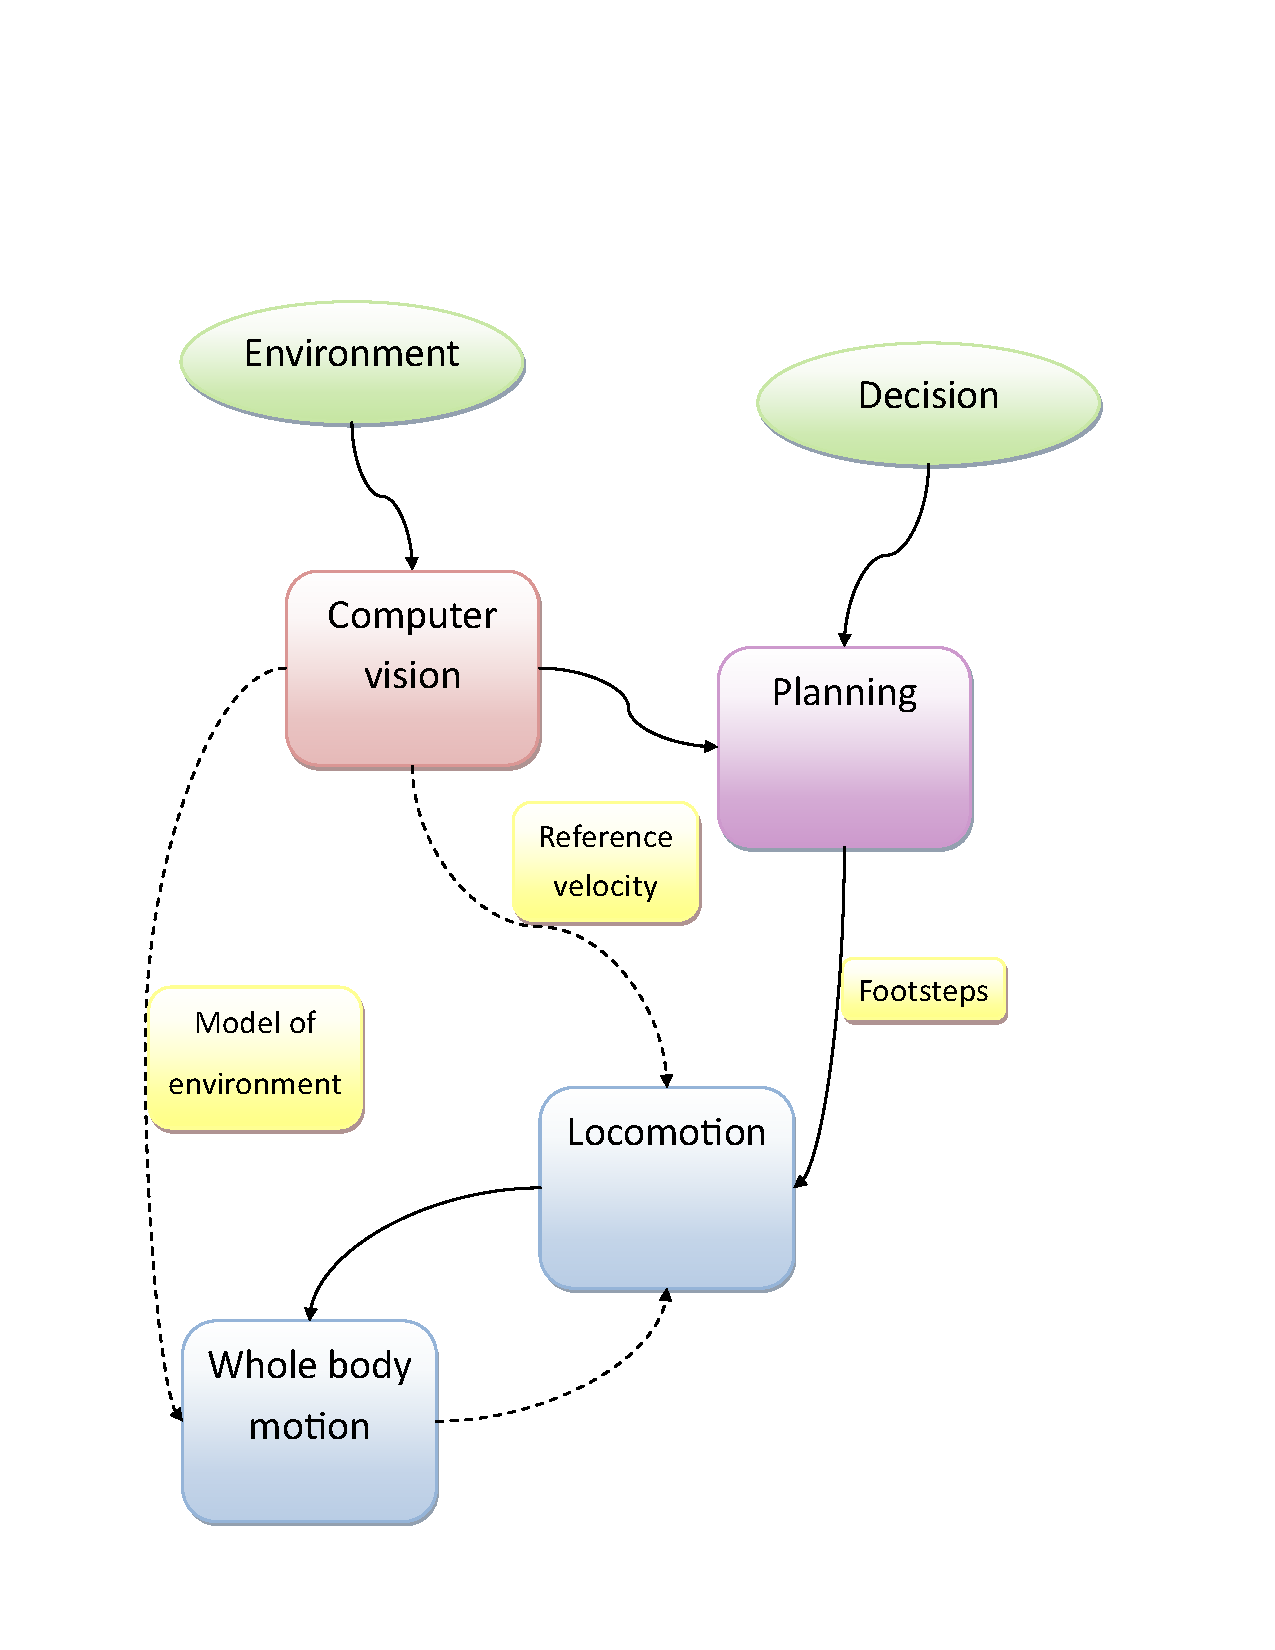
\includegraphics[scale=0.5]{Chap1-Introduction/general-diagram.pdf}
\caption[]{ \label{Fig:GeneralDiagram} Workflow of a humanoid robot executing motion tasks using perception.}
\end{figure}

In this thesis we address the problem of the link between vision and motion generation, as illustrated in Fig~\ref{Fig:PhotosVS}. Building upon the work of several authors through the years, our main contributions are,

\begin{itemize}
\item The full integration of a visual servoing scheme within the walking motion generation using Linear Model Predictive Control (MPC);
\item The integration of traditional motion planning approaches and on-line locomotion generation algorithms;
\item The visual reconstruction of 3D models of the scene in front of the robot to be used by an inverse-dynamics based approach to walk on rough terrain;
\item And finally, the validation in simulation of the proposals.
\end{itemize}

\begin{figure}[h!]
\centering
\subfigure[]{
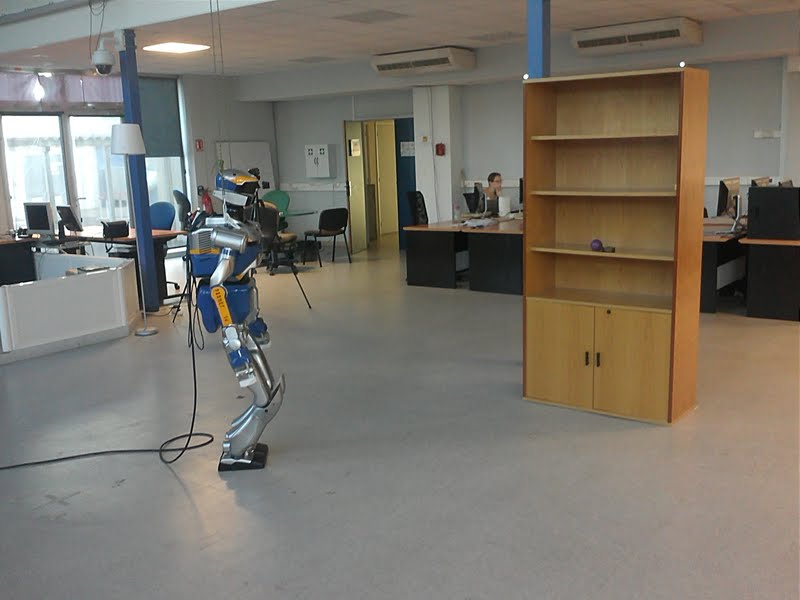
\includegraphics[scale=0.3]{Chap1-Introduction/hrp_2_setup.jpeg}}
\subfigure[]{
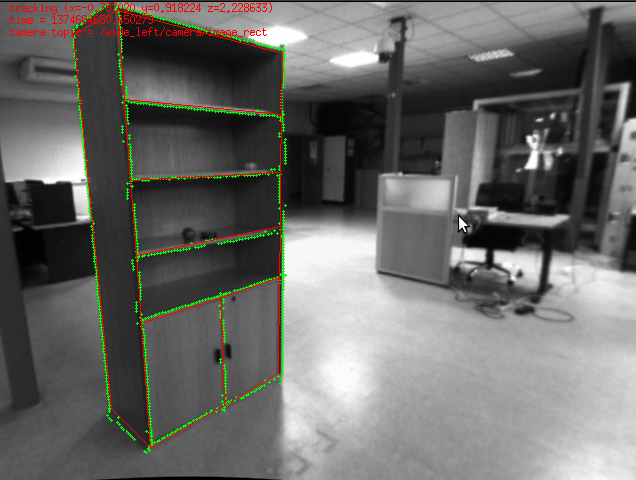
\includegraphics[scale=0.375]{Chap1-Introduction/visp_tracker_hrp2_big_shelf.png}}
\caption[]{ \label{Fig:PhotosVS} Typical application of computer vision and control, visual servoing.}
\end{figure}


The rest of this manuscript is organized as follows. In chapter \ref{Chap:Related-Work}, we state the problem and briefly recall the work that has been done on it. In chapter \ref{Chap:Locomotion-Control}, we introduce the techniques that most of the current walking motion generation schemes for humanoid robots are based on. The one proposed in Kajita et al. in 2003 \citep{Kajita2003} that focuses in the trajectory of the center of mass to generate balanced and stable motions and the one proposed by Herdt et al. in 2010 \citep{HerdtAR2010} in which a reference velocity is tracked. In chapter \ref{Chap:Visual-Servoing} we present an approach to introduce visual information in the walking pattern generator for humanoid robots. We make use of visual servoing with Model Predictive Control (MPC), which is combined with the walking motion generator. Since visual servoing with MPC is in general a nonlinear optimization problem, we propose a linearization scheme in order to keep it as a Quadratic Program (QP) and introduce it within the pattern generator. In chapter \ref{Chap:Visual-Planning}, we propose a method for reactive walking allowing visual servoing and adaptation of footsteps trajectories in real-time. This is done by building upon recent advances in the fields of optimal control for a walking pattern generator~\citep{HerdtAR2010} and planning for a nonholomic robot with field-of-view constraints ~\citep{Salaris:2010}. In chapter \ref{Chap:3DReconstruction}, we present a 3D reconstruction system of the ground in front of the robot. This model allows to know the ground structure where the swinging foot is going to step on to an inverse dynamics control scheme. Finally, in chapter \ref{Chap:Conclusions}, we present the final discussion and future work.




% State of the Art
%\begin{savequote}[10cm]
%{\it ``Part of the inhumanity of the computer is that, once it is competently programmed and working smoothly, it is completely honest.''}
%\qauthor{Isaac Asimov}
%\end{savequote}

\chapter{Related work} 
\label{Chap:Related-Work}

Recently, very efficient control systems for humanoid robots walking generation have been proposed.
They use dynamical balance criteria such as the Center Of Pressure (CoP) and may be very reactive since foot step placement can be computed online \citep{HerdtAR2010}. In this methodollogy the CoM and CoP trajectories and footstep positions are computed automatically. This result is fed to a whole-body controller to deal coherently with the three cases. Here, the notion of footsteps disappears, allowing the user to provide a reference velocity as input to the pattern generator. Moreover, because the range of footsteps is explored by a guided search in the space of the whole-body controller transitions, a large set of possible footsteps is available in real-time.

Most of these techniques are based on Linear Model Predictive Control (LMPC). LMPC previews the behavior of the system if one applies a sequence of controls and allows us to estimate the optimal control sequence for a given horizon. In the next iteration, one applies the first next optimal control. Remarkably, LMPC can be expressed as a Quadratic Program (QP), that is the minimization of quadratic errors subject to a set of constraints.
Handling explicitly the constraints in the QP is one of the main advantages of this formulation. 
Furthermore, there are very efficient techniques to solve QPs.

The next step would be to close the control loop and use sensors information as feedback, e.g. in positioning tasks. In general humanoid walking control assume that the robot foot steps are defined before computing the actual joint control to realize it. They generally follow a perception-decision-action scheme: footsteps on time horizon are defined upon sensors information on the environment, from the footsteps center of mass trajectories (CoM) are computed to respect balance constraints. Legs control is computed by inverse kinematics. This perception-decision-action loop has proven to be fast enough to realize impressive demonstrations for stair-climbing and obstacle avoidance \citep{Lorch02,Chestnutt07,Michel07,Guttmann08}. 

On the other hand, for reactive positioning tasks, visual servoing techniques have proven to be useful \citep{ChaumetteRAM2006, ChaumetteRAM2007}. Dune et al. \citep{DuneIROS2010} proposed a visual control scheme for humanoid robots using walking pattern generation as a black box. The desired velocity of the center of mass (CoM) is computed using visual servoing and it is used as a reference in the pattern generator. The main disadvantage with this approach is that the visual servoing scheme and the pattern generator are completely decoupled so the visual information is not directly feeding the pattern generator.

Visual servoing has been successfully applied in Model Predictive Control Schemes \citep{Allibert2010}. The main problem is that the dynamics of the camera and the projection itself are nonlinear functions for which non-linear programming are required. However, this may be time consuming and hence does not fit into an online walking pattern generator.

Parallely, research has been led towards planning trajectories that are appropriate for humanoid robots walking in cluttered environments, with different types of restrictions (e.g. \citep{Chestnutt2005, jib-IJHR2010}). 
From the seminal work of \citep{Chestnutt2005}, a main trend of research in footstep planning has been to consider a limited set of known actions (quite often footsteps) and transitions, and to find an optimal path over them. The use of a fixed-set-of-actions approach can be limiting, as it may produce unnecessary motions near the obstacles \citep{Bourgeot:IROS:2002}, while not usually dealing with the problem of robust perturbation rejection. 

A vast amount of work exist to lessen the amount of movements generated around the obstacles. Chestnutt et al. proposed in \citep{Chestnutt:ICRA:2007} an adaptation mechanism to search around the set of transitions. More recently, Hornung et al. \citep{Hornung:ICRA:2012}, proposed a method to deal with highly dynamical environments by keeping both, accurate short-term goals and rough long-term goals. As doing this may lead to local optima, the author propose a method to automatically adapt the set of actions according to the environment traversability characteristics. 

Regarding the problem of robust perturbation rejection, several advances have also been done. They can be divided into three strategies: (1) ankle-foot stabilization, (2) whole-body stabilization, and (3) footstep generation. 
Using the capture-point or the Center-of-Pressure (CoP) as an indicator of stability, one can switch between a Finite-State-Machine strategy~\citep{Nishiwaki:ijrr:2009} and a learned strategy \citep{SeungJoon:ichr:2011}.

From an application point of view, however, it is very difficult to decouple planning and control from each other. Planning is needed to avoid local optima and control is needed to reject disturbances and adapt to modeling errors. Some planning methods try to account for the motion and control capabilities of the humanoid robot by using inverse kinematics \citep{kanoun:ijrr:2011}. Despite real-time implementation \citep{Dang:ichr:2011}, this method suffers from local minima in planning footsteps. As in \citep{Vahrenkamp:IROS:2009}, we propose in this paper to use a planning approach integrating a constraint given by a task (e.g. visual-servoing). However, here, we modify the walking controller in such a way to use the planner as a generator of a full vector field that provides new local solutions from any given configuration and not only as a provider of single reference trajectories.


% State of the Art

\chapter{Locomotion} 
\label{Chap:Locomotion-Control}

In this chapter we introduce the techniques most commonly used in biped walking generation, the Linearized Inverted Pendulum Model and Kajita's Preview Control. These techniques are widely used and they have become a standard in humanoid walking control. In the next chapters, we will work upon these techniques. The reader is kindly encouraged to read the original papers to have a deeper understanding of these models.


\section{Models of Biped Walking and Kajita's Preview Control}
Most of the works in biped walking are based on the simplified model proposed by Kajita et al. in 1992 \citep{Kajita1992}. This model simplifies the multi-body nature of the robot considering it as a single mass moving as an inverted pendulum. This mass is moving in the $x,y$ plane. It also constraints the trajectory of the CoM to a horizontal plane, as depicted in Fig. \ref{Fig:Inverted-Pendulum}.

\begin{figure}
  \centering
      {\def\svgwidth{1.0\columnwidth}
        \subimport*{Chap3-Locomotion-Control/}
                   {inverted_pendulum.pdf_tex}}
      \caption[]{Humanoid walking modeled as an inverted pendulum. The center of mass is constrained to an horizontal plane. The ZMP corresponds to the point in the sole in which the momentum generated by the inertia and gravity is countered with the momentum generated by the contact forces of the foot with the ground.}
      \label{Fig:Inverted-Pendulum}
\end{figure}

The dynamics of this model is given by,

\begin{eqnarray}
\label{Eq:LIPM_dynamics}
\tau^a_x &=& mgc_y - mc_z \ddot{c}_y, \\
\tau^a_y &=& mgc_x - mc_z \ddot{c}_x
\end{eqnarray}

where $(c_x, c_y, c_z)$ is the 3D position of the CoM, $m$ its mass, and $\tau^a_x, \tau^a_y$ the torques produced by the inertia and gravity ($g$) in the base of the pendulum. We can note that the equation in the $y$ axis is completely equivalent to the $x$ axis.

In the contact of the sole with the ground, there exists the countering force $F^p$. The $x,y$ components of this force correspond to friction and avoid sliding. The $z$ component supports the weight of the pendulum and is equal to $F^p_z = mg$, as depicted in Fig.~\ref{Fig:Foot-Sole}.

\begin{figure}
  \centering
      {\def\svgwidth{0.5\columnwidth}
        \subimport*{Chap3-Locomotion-Control/}
                   {foot.pdf_tex}}
      \caption[]{The resultant forces and torques of the robot in the foot are $F^a$ and $\tau^a$ respectively. It corresponds the reactions in the contact with the floor. The resultant of those reactions is $F^p$ and its corresponding torque $\tau^p$. The $z$ component of this resultant $F^p_z$ corresponds to the vertical reaction of the floor. The $x$ and $y$ components correspond to friction forces and avoid sliding.}
      \label{Fig:Foot-Sole}
\end{figure}

The total torques in the base of the pendulum are given by,

\begin{eqnarray*}
\label{Eq:LIPM_total_torques}
\tau^{total}_{x} &=& \tau^p_x + \tau^a_x = F^p_z z^p_x + \tau^a_x, \\
\tau^{total}_{y} &=& \tau^p_y + \tau^a_y = F^p_z z^p_y + \tau^a_y
\end{eqnarray*}

where $(z^p_x, z^p_y)$ is the acting point of $F^p$.

The locomotion is dynamically balanced if the contact forces of the feet with the ground counter the forces due to the inertia and gravity. The Zero Moment Point (ZMP) $(z_x,z_y)$ corresponds to the point in the ground where the total moment in the base of the pendulum is equal to zero \citep{Vukobratovic1972,Vukobratovic2004},

\begin{eqnarray}
0 &=& m g z_x + \tau^a_x, \\
0 &=& m g z_y + \tau^a_y
\end{eqnarray}

substituting the former equations in equation \ref{Eq:LIPM_dynamics}, we derive the ZMP equations,

\begin{equation}
\label{Eq:LIPM_ZMP}
Z = 
\left[
\begin{matrix}
z_x \\ z_y
\end{matrix}
\right] = 
\left[
\begin{matrix}
c_x - \frac{c_z}{g}\ddot{c}_x \\ c_y - \frac{c_z}{g}\ddot{c}_y
\end{matrix}
\right].
\end{equation}

This model is equivalent to the cart-table model. See Fig. ~\ref{Fig:Inverted-Pendulum-Cart-Table}. This model simulates the dynamic of the robot as a running cart above a table. The cart is in a position where it is not statically stable, however, dynamically, if the cart accelerates in an appropriate way, inertia forces will keep it in balance.

\begin{figure}
  \centering
      {\def\svgwidth{0.5\columnwidth}
        \subimport*{Chap3-Locomotion-Control/}
                   {robot-cart-table1.pdf_tex}}
      \caption[]{Equivalent model for humanoid walking. Statically the table is not balanced, dynamically inertia forces balance the table.}
      \label{Fig:Inverted-Pendulum-Cart-Table}
\end{figure}

We take the control variables as the time derivative of the horizontal accelerations of the CoM,

$$
 u_x \stackrel{\mbox{\tiny def}}{=} \dfrac{d}{dt}\ddot{c}_x = \dddot{c}_x.
$$

From the  work of \citep{Kajita2003}, if we suppose that the trajectory has periodic piece-wise constant jerks on a time interval $T$, for discrete time $k$, we can express the CoM dynamics in the $x$-axis as,

$$
c_x(k+1) = c_x(k) + \dot{c}_x(k) T + \ddot{c}_x(k) T^2/2 + \dddot{c}_x(k) T^3/6.
$$

Let us define

$$
\hat{c}_x(k) \equiv 
\left[
\begin{matrix}
c_x(k) \\ 
\dot{c}_x(k)\\
\ddot{c}_x(k) 
\end{matrix}
\right]
$$ 

the state of the robot, defined by its position, velocity and acceleration at time $k$. 

We can express the state of the robot at time $k+1$ in terms of the state $k$ plus the control variable,

\begin{equation}
\label{Eq:state_dynamics}
\left(
\begin{matrix}
c_x(k+1) \\ 
\dot{c}_x(k+1)\\
\ddot{c}_x(k+1) 
\end{matrix}
\right) =
\left(
\begin{matrix}
1 & T & T^2/2 \\
0 & 1 & T \\
0 & 0 & 1
\end{matrix}
\right)
\left(
\begin{matrix}
c_x(k) \\ 
\dot{c}_x(k)\\
\ddot{c}_x(k) 
\end{matrix}
\right) +
\left(
\begin{matrix}
T^3/6 \\
T^2/2 \\
T
\end{matrix}
\right)
u_x(k).
\end{equation}

Finally, using Eq.~\ref{Eq:LIPM_ZMP} and Eq.~\ref{Eq:state_dynamics} we have the basic equations of biped locomotion,

\begin{equation}
\label{Eq:basic_dynamic_equations}
\left\{
\begin{array}{ccc}
 \hat{c}_x(k+1) &=&  A \hat{c}_x(k) + B u_x(k)\\
 z_x(k) &=& C \hat{c}_x(k)
\end{array}
\right.,
\end{equation}

with,

\begin{equation*}
 A = \left(
\begin{matrix}
1 & T & T^2/2 \\
0 & 1 & T \\
0 & 0 & 1
\end{matrix}
\right) \text{, }
{ B} = \left(
\begin{matrix}
T^3/6 \\
T^2/2 \\
T
\end{matrix}
\right) \text{ and }
{ C} = \left(
\begin{matrix}
1 \; 0 \; \dfrac{c_z}{g} \\
\end{matrix}
\right).
\end{equation*}

To solve this control system efficiently, Kajita et al. also  proposed to use Model Predictive Control (MPC). MPC takes into account future information by previewing the behavior of the system for a given horizon. Then, an optimization problem is formulated using a performance index,

\begin{equation}
\label{Eq:Performance-Index}
\min_{U(k)} \sum\limits_{i=k}^{k+N - 1} \frac{1}{2} Q (z_x(i+1) - z_x^{ref}(i+1))^2 + \frac{1}{2}R\dddot{c}_x^2(i),
\end{equation}

where $U(k) = [u(k)\hdots u(k+N-1)]$ is the sequence of the next $N$ controls, $z_x^{ref}(i)$ is a reference ZMP given by a previous footstep planning for instance, $Q$ and $R$ are constants and $N$ is the size of the horizon. The first term of the optimization problem contributes to a minimization of the squared error of the ZMP and the reference ZMP. The second term minimizes the jerks, so we can have smooth trajectories of the CoM.

The optimal controller is given by,

\begin{equation}
\dddot{c}_x(k) = -K_1 \sum\limits_{i=0}^{k} e(i)-K_2c_x(k) - \sum\limits_{j=1}^{N} K_p(j)z_x^{ref}(k+j)
\end{equation}

with $e(i) = z_x(i) - z_x^{ref}(i)$ being the ZMP error w.r.t. the reference ZMP, and $K_1$, $K_2$ and $K_p(j)$ are gains.

Kajita et al. also proposed a second step to correct the effects of the inverted pendulum simplification. This second step takes into account the multi-body dynamics and is re-injected to have better CoM and ZMP trajectories.

\section{Quadratic Programming and Automatic footstep placement}

Wieber in \citep{WieberHumanoids2006} proposed to reformulate the preview control problem as a Quadratic Programming Problem. By applying recursively the dynamics of Eqs.~\ref{Eq:basic_dynamic_equations}, we can express the position, velocity and acceleration  of the CoM in terms of the initial state $\hat{c}_x(k)$ and the sequence of jerks $\dddot{ C}_x(k) \stackrel{\mbox{\tiny def}}{=} \left[ \dddot{c}_x(k), \dddot{c}_x(k+1),...,\dddot{c}_x(k+N-1) \right]^{\transpose}$,

\begin{equation}
 \label{Eq:PosCMHorizon}
 {C}_x(k+1) \stackrel{\mbox{\tiny def}}{=}  \left(
 \begin{matrix}
  c_x(k+1) \\
  \vdots \\
  c_x(k+N-1)
 \end{matrix}
 \right) = {S}_p \hat{c}_x(k) + { U}_p \dddot{C}_x(k),
\end{equation}

\begin{equation}
 \label{Eq:VelCMHorizon}
 \dot{C}_x(k+1) \stackrel{\mbox{\tiny def}}{=}  \left(
 \begin{matrix}
  \dot{c}_x(k+1) \\
  \vdots \\
  \dot{c}_x(k+N-1)
 \end{matrix}
 \right) = {S}_v \hat{c}_x(k) + { U}_v \dddot{ C}_x(k),
\end{equation}

similar expressions can be obtained for the $y$ component. We can also express the ZMP trajectory,

\begin{equation}
 \label{Eq:PosZMPHorizon}
 { Z}_x(k+1) \stackrel{\mbox{\tiny def}}{=}  \left(
 \begin{matrix}
  {z}_x(k+1) \\
  \vdots \\
  {z}_x(k+N-1)
 \end{matrix}
 \right) = { S}_z \hat{c}_x(k) + { U}_z \dddot{ C}_x(k).
\end{equation} 

With the matrices $S_p, S_v, S_z \in \mathbb{R}^{N\times3}$ and $U_p, U_v , U_z \in \mathbb{R}^{N \times N}$ defined as,

\begin{equation*}
  S_{p}=\begin{bmatrix} 1 & T & T^2/2 \\ \vdots & \vdots & \vdots \\ 1 & NT & N^2T^2 \end{bmatrix}, \qquad
  U_{p}=\begin{bmatrix} T^3/6 & 0 & 0 \\ \vdots & \ddots & 0 \\ (1+3N+3N^2)T^3/6 & \cdots & T^3/6 \end{bmatrix},
\end{equation*}

\begin{equation*}
  S_{v}=\begin{bmatrix} 0 & 1 & T \\ \vdots & \vdots & \vdots \\ 0 & 1 & NT \end{bmatrix}, \qquad
  U_{v}=\begin{bmatrix} T^2/2 & 0 & 0 \\ \vdots & \ddots & 0 \\ (1+2N)T^2/2 & \cdots & T^2/2 \end{bmatrix},
\end{equation*}

\begin{equation*}
  S_{z} = \begin{bmatrix} 1 & T & \frac{T^2}2-\frac{z^{c}}{g} \\ \vdots & \vdots & \vdots \\
                          1 & NT & \frac{N^2T^2}{2}-\frac{z^{c}}{g} \end{bmatrix},
\end{equation*}

\begin{equation*}
  U_{z} = \begin{bmatrix}
            \frac{T^3}{6}-\frac{Tz^{c}}{g} & 0 & 0 \\
          \vdots & \ddots & \vdots \\
          [1+3(N-1)+3(N-1)^2]\frac{T^3}{6}-\frac{Tz^{c}}{g} & \cdots & \frac{T^3}{6}-\frac{Tz^{c}}{g}
          \end{bmatrix}.
\end{equation*}

This allows us to rewrite the optimization problem as,

\begin{eqnarray}
\nonumber
\underset{U(k)}{\min} ~~ \dfrac{1}{2} R \| \dddot{{C}}(k) \|^2 + \dfrac{1}{2} Q \|{Z}_x(k+1) - {Z}^{ref}_x(k+1) \|^2,
\label{Eq:MinJerk}
\end{eqnarray}
 
with the same interpretations as in Eq.~\ref{Eq:Performance-Index}.

This optimization problem has the analytical solution,

\begin{equation}
\dddot{{C}}_x(k) = -({U}_z^{\top} {U}_z + \dfrac{R}{Q} {I}_{N \times N})^{-1} {U}_z^{\top}({S}_z \hat{c}_x(k) - {Z}_x^{ref}(k+1)).
\end{equation}

Wieber showed that with this proposal the system is able to reject strong perturbations.

As an evolution of this work, where the footsteps positions (and, correspondingly, the ZMP reference) are fed to the pattern generation, the work of~\citep{HerdtAR2010} introduced automatic footstep placement, i.e. managed the footsteps as free variables in the optimization problem and not as inputs. This reduced the necessary input to a simple stack of reference velocities $(\dot{C}_{x}^{ref}(k+1),\dot{C}_{y}^{ref}(k+1))$. This leads to the optimization problem,

\begin{eqnarray}
\nonumber
 \underset{U(k)}{\min} \; && \dfrac{\alpha}{2} \left\| \dddot{C}_x(k) \right\|^2 + \dfrac{\alpha}{2} \left\| \dddot{C}_y(k) \right\|^2 \\
&& + \dfrac{\beta}{2} \left\| \dot{C}_{x}(k+1) - \dot{C}_{x}^{ref}(k+1) \right\|^2 + \dfrac{\beta}{2} \left\| \dot{C}_{y}(k+1) - \dot{C}_{y}^{ref}(k+1) \right\|^2  \nonumber \\
&& + \dfrac{\gamma}{2} \left\| Z_x(k+1) - Z_x^{ref}(k+1) \right\|^2 + \dfrac{\gamma}{2} \left\| Z_y(k+1) - Z_y^{ref}(k+1) \right\|^2,
\label{Eq:MinJerk}
\end{eqnarray}

with $\alpha$, $\beta$, $\gamma$ being constants that indicate the weight of each term in the optimization problem. The first two terms correspond to the minimization of the jerk, the next two terms correspond to a tracking of a reference velocity and the final ones correspond to a tracking of a reference ZMP.

The reference ZMP is defined as,

\begin{eqnarray}
\label{Eq:ZMPReference}
  Z_x^{ref}(k+1) & = V_c \hat{F}_x(k) + V F_x(k) \nonumber \\
  Z_y^{ref}(k+1) & = V_c \hat{F}_y(k) + V F_y(k),
\end{eqnarray}

with $\hat{F}_x(k)$, $\hat{F}_y(k)$ being the current position of the foot on
the ground.

The variables to optimize are

$$
U(k) \stackrel{\mbox{\tiny def}}{=} 
\left(
\begin{matrix}
\dddot{C}_{x}(k) \\
F_x(k) \\
\dddot{C}_{y}(k) \\
F_y(k)
\end{matrix}
\right),
$$

in which $F_x(k)$ and $F_y(k)$ are the next footstep positions in the horizon. In Eq.~\ref{Eq:ZMPReference} we set the reference ZMP to the middle of the support foot. This way, the reference ZMP is not fixed in advanced but is permanently recomputed from the feet position decided by the algorithm. Finally

\begin{equation*}
   V_c = \begin{bmatrix}1 \\ \vdots \\ 1 \\ 0 \\ \vdots \\ 0 \\ 0 \\ \vdots \\ 0  \end{bmatrix} \qquad
   V = \begin{bmatrix} 0 & 0 & 0 & \cdots & 0 \\ \vdots & \vdots
     & \vdots & \ddots\\ 
                                           0 & 0 & 0 & \cdots & 0\\
                           1 & 0 & 0 & \cdots & 0 \\ \vdots & \vdots &
                           \vdots &
                           \ddots \\ 1 & 0 & 0 &\cdots &0\\
                           0 & 1 & 0 & \cdots & 0\\ \vdots & \vdots &
                           \vdots & \ddots \\ 0 & 1 & 0 & \cdots &0\end{bmatrix},
\end{equation*}

are selection matrices that indicate which sampling time falls in which step.

As the terms in the optimization problem defined in Eqs.~\ref{Eq:PosCMHorizon}-\ref{Eq:PosZMPHorizon} and \ref{Eq:ZMPReference} are linear in the variables to optimize, the problem can be written as a Quadratic Program (QP),

\begin{equation}
 \underset{U(k)}{\min} \; \dfrac{1}{2} U(k)^{\transpose} Q(k) U(k) + p(k)^{\transpose} U(k),
\label{Eq:QP}
\end{equation}

under linear constraints arising, among others, from the inclusion of the reference ZMP inside the support polygon~\citep{HerdtAR2010}.

For instance, during the single support phase (in which we have a support foot and a flying one), the constraint ensuring that the ZMP remains inside the support polygon is expressed as:
\begin{equation}
  \begin{bmatrix} d_x(\theta) & d_y(\theta) \end{bmatrix}
  \begin{bmatrix} z_x - f_x \\ z_y - f_y \end{bmatrix} \leq b(\theta)
\end{equation}
where $(f_x,f_y)$ is the foot position, $\theta$ is its orientation,
$d_x(\theta)$, $d_y(\theta)$ are column vectors containing the $x$,
$y$ coordinates of the normal vectors to the feet edges, and $b(\theta)$  is the column vector containing their position with a security margin. For the double support phase, Herdt et al. chose to satisfy the constraint of the reference ZMP at the sampling time kT, and given that the double support phase is chosen to be T long (0.1s for the double support and 0.7 for the single support), no samplings fall strictly in the double support, so they just consider single support constraint in the reference ZMP. This assumption appears to be reasonable enough to generate stable motions as they showed in their experiments.

% Visual servoing
\chapter{Vision-Based Control of Humanoid Walking} 
\label{Chap:Visual-Servoing}

We have introduced the mathematical foundations behind humanoid walking. In this chapter we will discuss the applicability of controlling the robot trajectory using visual servoing, as depicted in Fig.~\ref{Fig:Schema}. We present a novel approach for using a visual servoing scheme to control the dynamic walk of a humanoid robot. Here, the online information given by an on-board camera is used to drive the robot towards a specific goal, in a visual servoing scheme. This closed loop approach allows the system to react to changes in its environment and to adapt to modeling errors. Our work is built upon the reactive pattern generator of \citep{HerdtAR2010} that we presented at the end of Chapter \ref{Chap:Locomotion-Control}, which modifies footsteps, center of mass and center of pressure trajectories to track a reference velocity. We compare our method to another which does not use Model Predictive Control in the visual servoing. This alternative method, proposed by Dune et al. \citep{DuneIROS2010} outputs, in a first stage, a reference velocity directly given by the visual servoing control law and then, in a second stage, this reference velocity is introduced in the pattern generator to produce the appropriate walking motion (hence, our term of ``decoupled''). The coupled approach proposed here uses a Model Predictive Control scheme to introduce the visual error terms directly within the pattern generator. This allows to avoid a number of limitations (e.g. that visual constraints cannot be introduced directly inside the locomotion controller or that the camera motion has to be accounted separately) that appear in the decoupled method.  In this work, both approaches are compared numerically and validated in simulation.

\section{ Visual servoing}

Visual servoing aims at controlling the motion of a robot equipped with a camera, by minimizing errors between observed features and their corresponding reference features, \citep{ChaumetteRAM2006, ChaumetteRAM2007}. The nature of the features differentiates schemes of visual servoing: Image based visual servoing (IBVS) uses only image features; Position based visual servoing (PBVS) uses the 3-D pose(s) of object(s) of interest. In any of these cases of feedback, one may use a velocity controller such as

$$
\text{v}^c = -\lambda {L}_e^{+} {e},
$$

\noindent where ${e} = {s}-{s}^{*}$ is the vector of errors between the current features $s$ and the desired ones ${s}^{*}$, $\text{{v}}^c$ is the velocity of the camera (the control variable), and ${L}_e^{+}$ is the Moore-Penrose pseudo-inverse of the interaction matrix ${L}_e$, that is, the matrix relating the velocity of the features and the velocity of the camera.

\begin{figure}[ht] 
\begin{center}
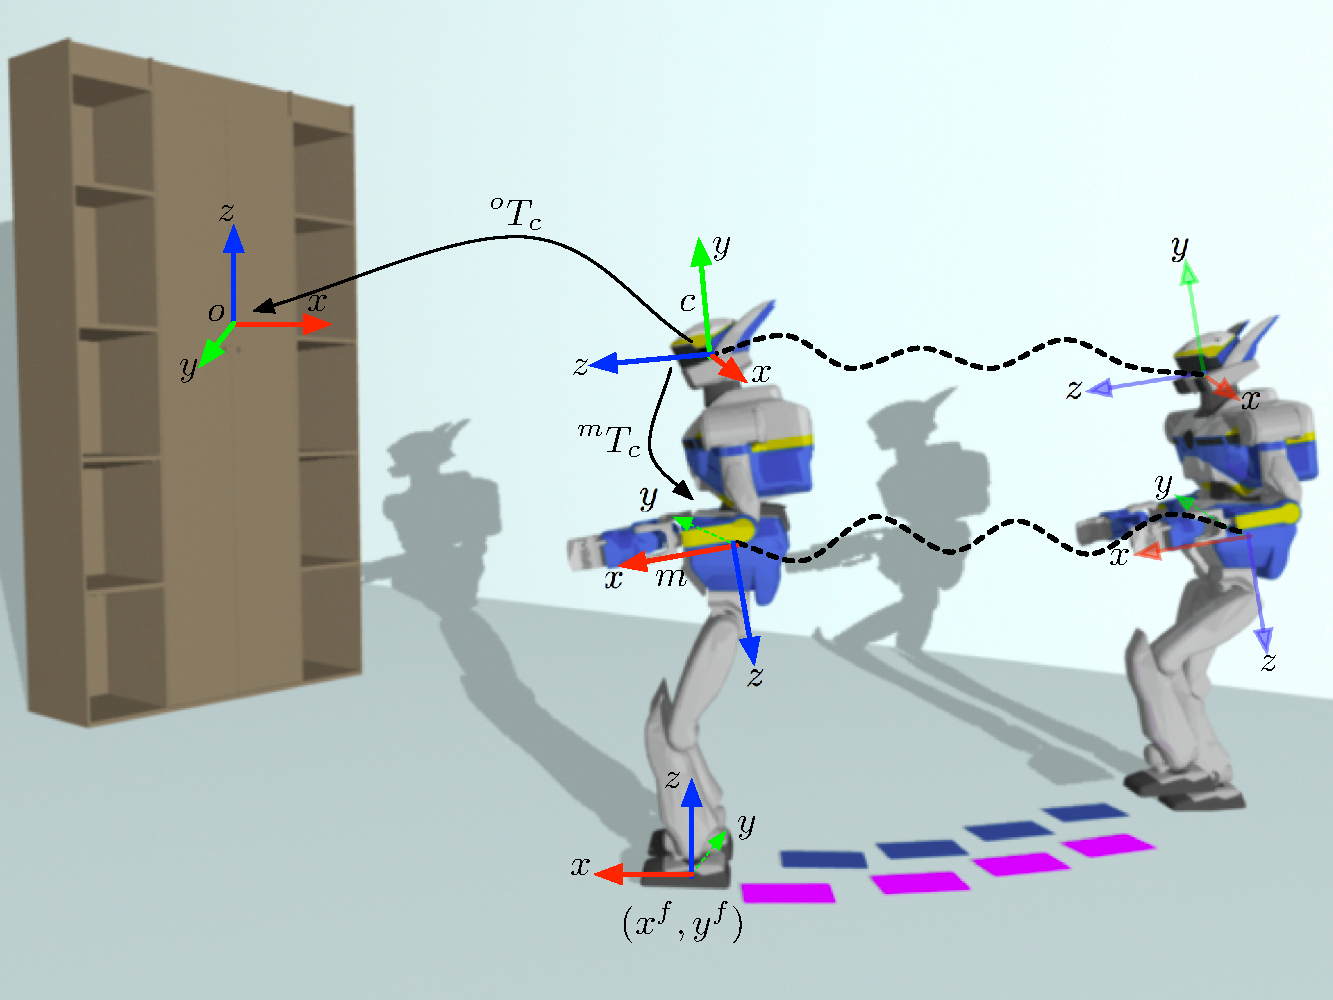
\includegraphics[scale=0.5]{Chap4-Visual-Servoing/schema_new.pdf} 
\caption{ An example setup for our approach: the robot has to walk towards a desired position with regards to an object viewpoint. Frames $o$, $c$ and $m$ refer to the {\it object}, {\it camera} and {\it CoM} respectively. $^o {T}_c$ is the transformation to view the camera points in the object reference frame. $(x^f, y^f)$ is the current footprint position.} 
\label{Fig:Schema}
\end{center}
\end{figure}

We will now describe two approaches for introducing visual control in the described pattern generation: the first one (in Section~\ref{sec:vsclaire}) is a decoupled one, proposed by Dune et al. \citep{DuneIROS2010}, where the visual servoing is used to determine the reference velocity in Eq.~\ref{Eq:MinJerk}; the second one (Section~\ref{sec:vsmauricio}) modifies Eq.~\ref{Eq:MinJerk} to replace the reference velocity term by a new term directly related to the decreasing of the visual errors.


\section{Visual Control Using a Reference Velocity}
\label{sec:vsclaire}


As for any pattern generator, the stepping motion induces a sway motion, which can be read as the difference existing between the reference velocity used in the Eq.~\ref{Eq:MinJerk} of the Model Predictive Control and the real velocity effectively attained from the first control. This sway motion is necessary for a proper walk, but it obviously generates non-desired effects on the robot visual perception. As stated in~\citep{DuneIROS2010}, the result of this sway motion on the real camera velocity $\text{v}^c$ can be modeled as:

\begin{equation}
\text{{v}}^c =\overline{\text{{v}}}^c+{^{c}  V_{m}} \text{{v}}^b
\label{eq:sway}
\end{equation}

\noindent where $\overline{\text{{v}}}^c$ is the ``ideal'' camera velocity that would exist without sway, and $\text{{v}}^b$ is the part of the CoM velocity that is induced by the sway. The matrix ${^c  V_{m}}$ is a $6\times6$ twist matrix relating the camera frame (index ``c'') to the CoM frame (index ``m'') through the transform ${^cT_{m}}$.

We recall how in~\citep{DuneIROS2010}, a classical visual servoing scheme is adapted to be used for a humanoid robot. The idea, basically, is to use the output velocity from Eq.~\ref{eq:avControlCom} as a reference velocity for Eq.~\ref{Eq:MinJerk}. However, as we have pointed it out, the humanoid motion has an intrinsic sway component, that makes the visual features have an evolution in the image not corresponding to the desired trajectory. 

As mentioned above, the features motion in the image can be decomposed into a component due to the sway motion, and a component due to the ``average'' (sway-less) motion of the robot,

\begin{equation}
\label{Eq:FeaturesSway}
\dot{ s}={ L_e} \overline{\text{v}}^c+ { L_e} \, ^c  V_{m}{\text{v}^{b}}.
\end{equation}

Then, the idea is to use a virtual camera that would correspond to the position of the camera if we supposed that there were no sway motion affecting the robot motion, to control this virtual camera, and use its controlled velocity ($\overline{\text{ v}}^c$) as a reference velocity in the reactive PG.
 
%----------------------FIG-----------------------------------------------%
%\begin{figure}[ht] 
%\begin{center}
%\includegraphics[width=\columnwidth]{images/correction.ps} 
%\vspace{-1cm} 
%\caption{ $\Rep{K}$ is the current camera frame and $\overline{\Rep{K}}$ is the camera position obtained if the visual servoing velocity is applied without the walking constraints.} 
%\label{fig:frames}

%\end{center}
%\vspace{-0.5cm} 
%\end{figure}
%------------------------------------------------------------------------%

Integrating equation \ref{Eq:FeaturesSway} between $0$ and $t$, Dune et al. have shown that the relationship between the real observed features $s(t)$ and the ``sway-less'' features $\bar{s}(t)$ can be written as

\begin{equation}
s(t) = \overline{s}(t) + \int_{0}^{t} {{\widehat{ L_e}}} \, ^c  V_{m} \text{ v}^b dt - E,
\end{equation}

\noindent where $E \stackrel{\mbox{\tiny def}}{=} s(0)-\overline{s}(0)$. From the previous equation, the corrected visual error between a reference features vector and the sway-less features vector, to be used for the computation of the reference velocity, is deduced as

\begin{align}
\overline{e}(t)&=\overline{s}(t) -s^*= e(t) -  (\int_{0}^{t}{ {\widehat{ L_e}}} \, ^c  V_m \text{ v}^b dt -E).
\end{align}

Under this model, the virtual error $\overline{e}(t)$ is regulated to zero, and the real error $e(t)$ is oscillating around zero, with a period $T$, because of the sway.

The shift $E$ is re-estimated regularly over one period of time (e.g., the last period) by 

$$
E= \frac{1}{T^{sway}}\int_{t-T^{sway}}^t\int_0^t { {\widehat{ L_e}}} \, ^c  V_m \text{ v}^b  dt dt,
$$ 

\noindent and finally, it is used in the control law for the CoM (e.g., the reference velocity for Eq.~\ref{Eq:MinJerk}) 

\begin{gather} 
\overline{\text{ v}}^m= -\lambda{ ^c  V_m {{ {\widehat{ L_e}}}}^{+}}(e -  (\int_{0}^{t}{{ {\widehat{ L_e}}}} \, ^c  V_{m}\text{ v}^b dt - E)).
\label{eq:avControlCom} 
\end{gather} 

Note that the discrete form of the involved integrals are used in practice. More details can be found in~\citep{DuneIROS2010}. To apply this control, we need the actual measured errors $ e$ (as in any classical visual servoing approach), an estimate of the sway motion period, which is deduced from the stepping period, and a point-wise estimate for the sway motion at the level of the CoM $\text{ v}^b$.

This reference velocity can be directly injected in the Velocity Controlled Pattern Generator introduced in previous section. However, this approach has several drawbacks. First, the control law will never be executed as is, because of dynamical and physical limitations of the robot. Second, to get equation \ref{eq:avControlCom}, they make several assumptions, which sometimes are not true. And third, since the PG and the servo controller are totally decoupled, the visual feedback has to wait for the next iteration to be introduced in the PG. In order to solve this problem, we will present in the next section a Visual Servo controller which will be directly introduced in the Pattern Generator.

\section{Visual servoing and MPC}
\label{sec:vsmauricio}

As we know, in walking pattern generation, MPC is used to estimate a sequence of optimal controls at some horizon, because of the step-based nature of walking. Hence, we want to orient the optimization of the foot placement by taking into account the expected evolution of the visual servoing (VS) errors so that, instead of minimizing the VS errors at current time $k$, one would like to foresee its evolution at some horizon $[k+1,k+N]$. In this chapter, in order to simplify the notation, we will use the form $s_k$ to express the time reference $k$ of $s(k)$ and alike.

In~\citep{Allibert2010}, such a time horizon-aware scheme has been proposed. The visual predictive control (VPC) is introduced as:

\begin{eqnarray}
\label{Eq:MinVisualFeatures}
 \min_{U_{k}} \;&& \sum\limits_{j=k+1}^{k+N} [ s^d_j - s^m_j]^{\transpose} W_j [s^d_j - s^m_j], \\
 \mbox{subject to} \; && s^d_j = s^{*}_j - \epsilon_j, \\
 \label{Eq:ConstraintDynamicModel}
 && q_j = f(q_{j-1},u_{j-1}), \\
 \label{Eq:ConstraintProjection}
 && s^m_j = h(q_j).
\end{eqnarray}

In Eq.~\ref{Eq:MinVisualFeatures}, $U_{k}=u_{k:k+N-1}$ are the series of controls to be applied, $q_j$ is the state, and $s^*_j$, $s^d_j$ and $s^m_j$ are respectively the reference, desired and predicted positions of the visual features. The terms $\epsilon_j$ are the errors $s_j-s^m_j$ between real and predicted feature positions.
Allibert et al. assume $\epsilon_j$ constant over the prediction horizon, equal to $\epsilon_k=s_k-s^m_k$, i.e. the error at current time $k$, because by definition the $s_j$ are not known for $j>k$.
Since our landmarks are static, $s^*_j \stackrel{\mbox{\tiny def}}{=} s^*$, and since the prediction errors are constant on the horizon window, $s^d_j=s^d_k=s^*-\epsilon_k$ are constant in the prediction horizon.

Eq.~\ref{Eq:ConstraintDynamicModel} is the dynamic model, that estimates the new state given the last state/control pair. In general, this function is non-linear. We will see how to deal with this non-linearity.

Eq.~\ref{Eq:ConstraintProjection} is also a non-linear function that estimates the output of the model $s^m_j$, given the current state $q_j$. This equation implements the pinhole camera projection model.

Matrix $W_j$ in Eq.~\ref{Eq:MinVisualFeatures} is a positive definite matrix  used to weight errors in the prediction horizon. As suggested in~\citep{Allibert2010}, we   consider equal weights for all features errors, $W_j = diag(w_j)$. 

Here, $s^m_j$ is the collection of all the predicted features at time $j$, that is, for $M$ features $s^m_j = ( s_{1,j}^m, s_{2,j}^m, \hdots, s_{M,j}^m )^{\transpose} $. Eq.~\ref{Eq:MinVisualFeatures} can be rewritten as

\begin{equation}
\label{Eq:MinVisualFeatures2}
 \min_{U_{k}} \; \sum\limits_{l=0}^{M}  [S^d_{l} - S^m_{l,k}]^{\transpose} W [S^d_{l} - S^m_{l,k}],
\end{equation}

\noindent with $S^m_{l,k} =  \left(
  s^m_{l,k+1},
  s^m_{l,k+2},
 \dots,
  s^m_{l,k+N}
 \right)^{\transpose}$ stacking the features positions in the horizon, $S^d_{l}$ stacking the corresponding desired positions, and the weights matrix $W = diag(w_{k+1},w_{k+2},...,w_{k+N})$.

Allibert et al. solved directly the non-linear programming problem Eqs.~\ref{Eq:MinVisualFeatures}-\ref{Eq:ConstraintProjection} to compute the controls in their visual servoing scheme.

\section{Integrating the visual servoing to the walking motion generator}
\label{sec:integration}
In the following we use superscripts $w,c,m$ to refer the world, the camera, and the CoM reference frame, and $T^{cm}$ means transformation from $c$ to $m$ frame. If we introduce directly Eq. \ref{Eq:MinVisualFeatures2} in Eq. \ref{Eq:MinJerk}, we will not have a QP anymore due to the non-linear constraints, namely Eqs. \ref{Eq:ConstraintDynamicModel} and \ref{Eq:ConstraintProjection}. We can directly solve the first problem (Eq. \ref{Eq:ConstraintDynamicModel}) by using the dynamic model in Eq. \ref{Eq:PosCMHorizon}. In this case there is no rotation, but we will see that we can introduce it in a decoupled way without losing the QP formulation.

\subsection{Linearization of the observation model}

As we said, Eq. \ref{Eq:ConstraintProjection} implements the pinhole camera model. Let $p^{w}_{l'} = [x^{w}_{l'},y^{w}_{l'},z^{w}_{l'}]^{\transpose}$ be the position of the {l'}-th landmark in the world reference frame. At time $j$, one can compute the projection to the image plane by first transforming the landmark position to the camera frame with the homogeneous transform $T^{mc} T^{wm}_j$ and then applying the projection,

\begin{equation}
\label{Eq:Projection}
\begin{array}{c}
 \left(
 \begin{matrix}
  u_{l',j} \\
  v_{l',j}
\end{matrix}
\right)
  =
 \left(
 \begin{matrix}
  u(x^{c}_{l',j},y^{c}_{l',j},z^{c}_{l',j}) \\
  v(x^{c}_{l',j},y^{c}_{l',j},z^{c}_{l',j})
 \end{matrix}
 \right)
 =  \left(
 \begin{matrix}
  x^{c}_{l',j} / z^{c}_{l',j}\\
  y^{c}_{l',j} / z^{c}_{l',j}
 \end{matrix}
 \right),
 \end{array}
\end{equation}

\noindent where $T^{wm}_j$ is the transformation from the world frame to the CoM frame and $T^{mc}$ is the transformation from the CoM frame to the camera frame, which is not variable in our approach. Note that

$$
T^{wm}_j = (T^{mw}_j)^{-1} = 
\left(
\begin{matrix}
(R^{mw}_j)^{-1} & -(R^{mw}_j)^{-1}t^{mw}_j \\
0_{1 \times 3} & 1
\end{matrix}
\right)
$$ 

\noindent where $t^{mw}_j$ is the position of the CoM in the world frame at time $j$, which depends in our control variables through Eq. \ref{Eq:PosCMHorizon}.
$R^{mw}_j$ is the direction of the robot waist according to the world reference frame at time $j$. In our current formulation 
there is no free variables modifying this quantity, because it would make the problem non-linear. More details
about this problem are given in Section~\ref{subsection:control_of_the_rotation_angle}.

If we use directly Eq. \ref{Eq:Projection} (non-linear), we will lose the QP formulation. 
We know that Eq.~\ref{Eq:Projection} is a projection $h:\mathbb{R}^3 \rightarrow \mathbb{R}^2$.

\begin{equation*}
%\label{Eq:ProjectionTaylor}
h(x,y,z) =
 \left(
 \begin{matrix}
  u(x,y,z) \\
  v(x,y,z)
 \end{matrix}
 \right)
 = \left(
 \begin{matrix}
  x / z\\
  y / z
 \end{matrix}
 \right).
\end{equation*}


We also know from MPC that prediction is done over a finite horizon. So it might be enough to use a first order approximation of $h$ for small $(dx,dy,dz)$ so that we can maintain the QP form.

Now, by using a Taylor series for $u(x,y,z)$ around some point $(x_0,y_0,z_0)$ and substituting the derivatives,

%$$
%\begin{array}{c}
% u(x_0+dx,y_0+dy,z_0+dz) = u(x_0,y_0,z_0) +\\
% u_x(x_0,y_0,z_0)dx + u_y(x_0,y_0,z_0)dy + \\
% u_z(x_0,y_0,z_0)dz + \mathcal{O}(dx,dy,dz)^2
%\end{array}
%$$

$$
\left\{
\begin{array}{c}
%\label{Eq:ProjectionTaylorApproxU}
\nonumber
 u(x_0+dx,y_0+dy,z_0+dz) \approx \dfrac{x_0}{z_0} +  \dfrac{dx}{z_0} - \dfrac{x_0 dz}{z_0^2},\\ \\
 v(x_0+dx,y_0+dy,z_0+dz) \approx \dfrac{y_0}{z_0} +  \dfrac{dy}{z_0} - \dfrac{y_0 dz}{z_0^2}.
\end{array}
\right.
$$

\noindent with $dx=x-x_0$, $dy=y-y_0$ and $dz=z-z_0$. 

We propose to apply such a linearization of Eq.~\ref{Eq:Projection} for the whole horizon, around the first position $(j=k)$ of landmark $l'$, i.e. at the linearization point $(x^{c}_{l',k},y^{c}_{l',k},z^{c}_{l',k})$, that is, the point we are actually watching, in the CoM frame. 

This way, we can express the predicted position of the landmark $l'$ linearly at time $j>k$ in the horizon:

\begin{equation*}
%\label{Eq:ProjectionLinearized}
 \left(
 \begin{matrix}
  u_{l',j} \\
  v_{l',j}
 \end{matrix}
 \right)
 = \left(
 \begin{matrix}
  \pi^{11}_{l',k} x^{c}_{l',j} + \pi^{13}_{l',k} z^{c}_{l',j}+ u_{l',k}\\
  \pi^{22}_{l',k} y^{c}_{l',j} + \pi^{23}_{l',k} z^{c}_{l',j} + v_{l',k}
 \end{matrix}
 \right),
\end{equation*}

\noindent where $u_{l',k} = x^{c}_{l',k} / z^{c}_{l',k}$ and $v_{l',k} = y^{c}_{l',k} / z^{c}_{l',k}$ are the initial image positions of the landmarks in the horizon and the coefficients $\pi^{ij}_{l',k}$ the elements of the matrix

\begin{equation*}
\Pi_{l',k} = \left(
\begin{matrix}
 1/z^{c}_{l',k} & 0 & - u_{l',k} / z^{c}_{l',k} \\
 0 & 1/z^{c}_{l',k} & - v_{l',k} / z^{c}_{l',k}
\end{matrix}
\right),
\end{equation*}

\noindent which is the classical definition of the interaction matrix in Image-Based Visual Servoing.

Finally, we can express the projection of the $l'-th$ landmark (constraint \ref{Eq:ConstraintProjection}) as:

\begin{equation}
\label{Eq:Features}
 \left(
 \begin{matrix}
  u_{l',j} \\
  v_{l',j}
 \end{matrix}
 \right) = 
\left[
\begin{array}{cc}
\multirow{2}{*}{$\Pi_{l',k}$} & u_{l',k} \\
& v_{l',k} \\
\end{array}
\right]
 T^{mc} T^{wm}_j \left( \begin{array}{c}
 p^{w}_{l'}\\
 1
 \end{array}\right),
\end{equation}

\noindent so that we can now introduce the visual features in the pattern generator. Expanding terms in Eq.~\ref{Eq:Features} for the first row and setting $\Pi^u_{l',k}$ as the first row of matrix $\Pi_{l',k}$,

\begin{eqnarray}
\label{Eq:FeatExpanded}
 u_{l',j} &= &\Pi^u_{l',k} (R^{wc} p^{w}_{l'} + R^{wc} t^{mw}_j + t^{mc}) + u_{l',k}.
\end{eqnarray}

Since $R^{wc} t^{mw}_j = R^{wc}_1 x_j + R^{wc}_2 y_j + R^{wc}_3 z_j$, where $R^{wc}_i$ is the $i$-th column of $R^{wc}$
\footnote{To simplify the notations $R^{wc}=R^{mc}R_j^{wm}$}
and $x_j,y_j,z_j$ the position of the CoM at time $j$ (see Chapter~\ref{Chap:Locomotion-Control}). We can rewrite Eq.~\ref{Eq:FeatExpanded}

\begin{equation}
\label{Eq:FeaturesUReduced}
 u_{l',j} = a^u_{l',k} x_j + b^u_{l',k} y_j + c^u_{l',k},
\end{equation}

\noindent with 
$$
\left\{
\begin{array}{ccl}
a^u_{l',k} & = & \Pi^u_{l',k} R^{wc}_1\\
b^u_{l',k} & = & \Pi^u_{l',k} R^{wc}_2\\
c^u_{l',k} & = & \Pi^u_{l',k} (R^{wc} p^{w}_{l'} + t^{mc} + R^{wc}_3 z_j) + u_{l',k}.
\end{array}
\right.
$$
Equivalently,

\begin{equation}
\label{Eq:FeaturesVReduced}
  v_{l',j} = a^v_{l',k} x_j + b^v_{l',k} y_j + c^v_{l',k}.
\end{equation}

Stacking the features $u_{l',j}$ and the CoM positions for the whole horizon and using Eq.~\ref{Eq:PosCMHorizon}, we get a vector $S^m_{l,k}$ similar to the one introduced in Eq.~\ref{Eq:MinVisualFeatures2} 

\begin{equation*}
S^m_{l',k} = A^u_{l',k} C_x(k+1) + B^u_{l',k} C_y(k+1) + C_{l',k}^u,
\end{equation*}

\noindent with 
$$
\begin{array}{ccl}
A^u_{l',k} &=& a^u_{l',k} I_{N\times N}\\
B^u_{l',k} &=& b^u_{l',k} I_{N\times N}\\
C_{l',k}^u &=& c^u_{l',k} (1,1,...,1)^{\transpose}
\end{array}
$$

 \noindent which corresponds to the predicted coordinates $u$ of the landmark $l'$-th in the horizon.
The equivalent equations for the $v$ coordinates of the same landmark are straightforward.

Every projected landmark provides two coordinates $(u,v)$ and we treat each one as an individual feature. This means that the $l$-th feature is the $u$ coordinate in the image of the landmark $l' = \left \lfloor l/2 \right \rfloor$ for $l$ even, and the $v$ coordinate for $l$ odd.

Generalizing to all features, we have:
\begin{equation}
\label{Eq:FeaturesStacked}
 S^m_{l,k} = A_{l,k} C_x(k+1) + B_{l,k} C_y(k+1) + C_{l,k},
\end{equation}

\noindent with $A_{l,k} = A^u_{l',k}$ for $l$ even and $A_{l,k} = A^v_{l',k}$ for $l$ odd. The same holds for $B_{l,k}$ and $C_{l,k}$.

Finally, we can introduce visual servoing in the walking generation with the QP:

\begin{eqnarray*}
\label{Eq:MainQP}
\nonumber
 \min_{U(k)} \; && \dfrac{\alpha}{2} \left\| \dddot{C}_x(k) \right\|^2
 + \dfrac{\gamma}{2} \left\| Z_x(k+1) - Z_x^{ref}(k+1) \right\|^2 \\
 \nonumber
 && + \dfrac{\alpha}{2} \left\| \dddot{C}_y(k) \right\|^2
 + \dfrac{\gamma}{2} \left\| Z_y(k+1) - Z_y^{ref}(k+1) \right\|^2 \\
 \nonumber
 && + \dfrac{\beta}{2} \sum\limits_{l=0}^{M}  [S^d_{l}- S^m_{l,k}]^{\transpose} W [S^d_{l} - S^m_{l,k}],
\end{eqnarray*}

and as a canonical QP:
\begin{equation*}
\underset{U(k)}{\min} \; \dfrac{1}{2} U(k)^{\transpose} Q(k) U(k) + p(k)^{\transpose} U(k)
\end{equation*}

\text{ with }
\begin{equation*}
Q(k) = \left( \begin{array}{cc}
Q(k)' & 0 \\
0 & Q(k)'
\end{array}
 \right) + \hat{Q}(k),
\end{equation*}

\begin{equation*}
 Q(k)' = \left(
 \begin{array}{cc}
 \alpha I + \gamma U^{\transpose}_{z}U_{z} & - \gamma U^{\transpose}_{z}V \\
 -\gamma V^{\transpose} U_{z} & \gamma V^{\transpose} V
 \end{array}
 \right),
\end{equation*}

\begin{equation*}
 \hat{Q}(k) = \left(
 \begin{matrix}
 \beta \sum\limits_l U_{p}^{\transpose} A_{l,k}^{\transpose} {W} A_{l,k} U_{p} & 0 & \beta \sum\limits_l U_{p}^{\transpose} A_{l,k}^{\transpose} {W} B_{l,k} U_{p} & 0\\
 0 & 0 & 0 & 0 \\
 \beta \sum\limits_l U_{p}^{\transpose} B_{l,k}^{\transpose} {W} A_{l,k} U_{p} & 0 & \beta \sum\limits_l U_{p}^{\transpose} B_{l,k}^{\transpose} {W} B_{l,k} U_{p} & 0 \\
 0 & 0 & 0 & 0
 \end{matrix}
 \right)
\end{equation*}

and $p(k) = p(k)' + \hat{p}(k)$,

\begin{equation*}
 p'(k) = 
 \left(
 \begin{array}{c}
 \gamma U^{\transpose}_{z}(S_{z} \hat{c}_x(k) - V_c \hat{F}_x(k) \\
 -\gamma V^{\transpose}(S_{z}\hat{c}_x(k) - V_c \hat{F}_x(k) ) \\
 \gamma U^{\transpose}_{z}(S_{z} \hat{c}_y(k) - V_c \hat{F}_y(k) ) \\
 -\gamma V^{\transpose} (S_{z}\hat{c}_y(k) - V_c \hat{F}_y(k) )
 \end{array}
 \right),
\end{equation*}

\begin{equation*}
 \hat{p}(k) = 
 \left(
 \begin{matrix}
 \beta  \sum\limits_l U_{u}^{\transpose} A_{l,k}^{\transpose} W [A_{l,k} U_{s} \hat{c}_x(k) + B_{l,k} U_{s} \hat{c}_y(k) + C_{l,k} - S^d_l]\\
 0 \\
 \beta  \sum\limits_l U_{p}^{\transpose} B_{l,k}^{\transpose} W [A_{l,k} U_{s} \hat{c}_x(k) + B_{l,k} U_{s} \hat{c}_y(k) + C_{l,k} - S^d_l ]\\
 0
 \end{matrix}
 \right).
\end{equation*}

One must note in Eq.~\ref{Eq:MainQP}, unlike the velocity controlled PG, this QP does not include the reference velocity tracking, instead, it includes the minimization of the visual errors. It also includes the terms of the minimization of the jerks and the ZMP centering.

\subsection{Control of the rotation angle}
\label{subsection:control_of_the_rotation_angle}

So far, we have proposed a scheme to control the trajectory of the center of mass in the $xy$ plane. However, introducing the rotation angle in the minimization problem is not straightforward without losing linearity. Furthermore, the rotation angle plays a very important role here since sometimes most of the error between the desired features $s^d$ and the predicted features $s^m$ may be due to the angle between the robot and the features.

An extension of the original linear MPC scheme with automatic footstep placement that deals with a reference angular velocity has been proposed in~\citep{HerdtIROS2010}. The approach is a decoupled solution, that is, it estimates first the optimal rotation angles and afterwards introduces these values as known in the main QP (as the matrix ${R^{mw}_{j}}$). This scheme should not affect the stability of the walking since inertial effects are not taken into account.

The same decoupled solution is used in this approach. Hence, in a first stage, we optimize the orientations in the MPC time window by  

{\small
\begin{eqnarray}
 \min\limits_{\dddot{C}_{\theta}(k),\dddot{F}_{\theta}(k) }  &&  \dfrac{\beta}{2} \left\| C_{\theta}(k+1) - \Theta^{0} \right\|^2 + \dfrac{\gamma}{2} \left\| F_{\theta}(k+1) - \Theta^{0} \right\|^2 \\
\nonumber && + \dfrac{\alpha}{2} \left\| \dddot{C}_{\theta}(k) \right\|^2 + \dfrac{\alpha}{2} \left\| \dddot{F}_{\theta}(k) \right\|^2,
\end{eqnarray}
}

\noindent with the same notations as for $\dddot{C}_x(k)$ and $\dddot{C}_y(k)$, $\dddot{C}_{\theta}(k)$ is the sequence of $N$ jerk values to be applied, and $C_{\theta}(k+1)$ is the sequence of predicted $\theta$ values, i.e. the orientations of the trunk,  

$$
C_{\theta}(k+1) \stackrel{\mbox{\tiny def}}{=} (c_{\theta}(k+1),...,c_{\theta}(k+N))^{\transpose},
$$

\noindent and similarly for $F_{\theta}(k+1)$, the feet orientations. Finally, as a reference orientation $\Theta^{0}$ is defined once for all at the starting configuration as a target feet orientation. Several conventions exist, in this paper, the trunk orientation $C_{\theta}(k)$ is trying to follow the flying foot orientation $F_{\theta}(k)$. The flying foot is the only one which can move during the single support phase. Certainly, the support foot is fixed, and both feet are fixed during the double support phase. Finally, zero speed, and zero acceleration are specified at the beginning and the end of the trajectories.

Then in a second stage, we introduce these angles as constant in the main QP (Eq.~\ref{Eq:MinJerk}). This approach gives us the advantage of introducing the following constraints,

\begin{eqnarray}
\label{Eq:RotConstFT}
| C_{\theta}(k+1) - F_{\theta}(k+1)| < \Theta^{FT}_{max} \\
\label{Eq:RotConstLR}
| C_{\theta}^{f,L}(k+1) - C_{\theta}^{f,R}(k+1)| < \Theta^{LR}_{max} \\
\label{Eq:RotConstVis}
| C_{\theta}(k+1)| < \Theta^{visibility}.
\end{eqnarray}

Eq.~\ref{Eq:RotConstFT} constraint the maximum rotation between feet and trunk, Eq.~\ref{Eq:RotConstLR} between both feet, and Eq.~\ref{Eq:RotConstVis} sets a rotation limit of the trunk to keep the visibility of the landmarks.

\subsection{Visual constraints}


The introduction of visual constraints can be done by using Eq.~\ref{Eq:FeaturesUReduced} and Eq.~\ref{Eq:FeaturesVReduced}. Any linear constraint in the image plane $(u,v)$, can be expressed as a linear constraint in the variables $U(k)$.

Furthermore a convex polytope can be expressed under a linear form. It means that we can have time- and landmark-varying constraints. Commonly we only want all landmarks to follow trajectories inside of some convex polytope. Hence, constraints become constant in time and for all landmarks. This can be written as:

\begin{eqnarray}
  A'
 \left(
 \begin{matrix}
  A^u_{l',k} C_x(k+1) +  B^u_{l',k} C_y(k+1) +  C^u_{l',k} \\
  A^v_{l',k} C_x(k+1) +  B^v_{l',k} C_y(k+1) +  C^v_{l',k}
 \end{matrix}
 \right) &\leq&  b'
 \label{Eq:VSConstraintsOptimVar}\\
\nonumber
\text{and then,} ~  A'' U_k &\leq&  b'',
\end{eqnarray}

\noindent where matrix $ A'$ and vector $ b'$ are related with the image constraints. For example, bound constraints in the $(u,v)$ coordinates like visibility constraints are easily expressed in terms of Eq.~\ref{Eq:VSConstraintsOptimVar} and are introduced directly in the QP.


\subsection{Qualitative comparison with the classical approach}

\label{subsection:qualdiscussion}

A first advantage of introducing the visual errors term in the Pattern Generator MPC and of avoiding the decoupled approach is that with a pure visual servoing approach, the expected behavior of the controls to be applied would correspond to an exponentially decreasing velocity, with velocities that eventually could not be realized by the humanoid robot. On the opposite, with our approach, because the visual errors term is only one term in the QP problem (1) the exponential decay is attenuated by the regularizing effect of other terms such as the jerks and (2) the constraint on velocities (maximal velocities) are naturally handled.   

Moreover, since the velocity reference we set as an input to the pattern generator is not truly performed (due to physical constraints of the robot), we have to re-inject this difference in the next iteration. In the coupled approach those problems are handled intrinsically within the Model Predictive Control. The sway motion is naturally filtered since we minimize the errors within a full cycle (the horizon in the Model Predictive Control). Finally, in the MPC-based coupled approach, we minimize errors as long as the stability criteria permits it, so we always request (and apply) feasible controls and the error is instantaneously taken into account.

Finally, we know classical visual servoing control laws have very good performance in robotic arms. However, stepping is a highly dynamic process. We can not ignore the stability and limitations in the design of our control laws. For instance, in classical visual servoing, while reaching the goal, the velocity controls requested to the robot are getting smaller, and null velocities are theoretically reached at infinite time, due to the exponential decay. Clearly we stop the motion when some convergence criteria is reached. This is not a problem with robotic arms since we just send rotational velocities to the motors, so this velocity can be very small. On the other side, the motion can take long time, and the stability of the robot arm system is not jeopardized. Stepping involves balance, and every step could break it. We must avoid unnecessary motion and reach the goal as soon and efficient as possible.


\section{Simulation results}

\subsection{Simulation results on the MPC-based approach only}

We first tested our own approach (Section~\ref{sec:vsmauricio}) in a simulated environment with the HRP-2 robot model and we comment these results hereafter. We assume that no noise or modeling errors have been introduced. For all the tests, the initial position is $(0,0)$ and the desired features are set in the position $(2,1)$. First, we try with a desired final position that does not imply rotation, so that the robot has just to control the $x$ and $y$ velocities, which are the variables in the QP. Depending of the weights of the QP, we obtain different trajectories, such as in Figs.~\ref{Fig:Results1} and \ref{Fig:Results2}. The difference between these two simulations is that we increased the $\beta $ parameter ($\beta=0.001$ in the first, $\beta =0.005$ in the second). The result is that the robot minimizes first the visual features errors, disregarding the jerks regularization term, which produces higher velocities and a globally less smooth trajectory.

%% Needs more descriptions of the figures. Ex: what are the two curves in 1.c ?

\begin{figure*}[h]
\begin{minipage}{0.5\textwidth}
 \centering
  %\subfigure[]{
 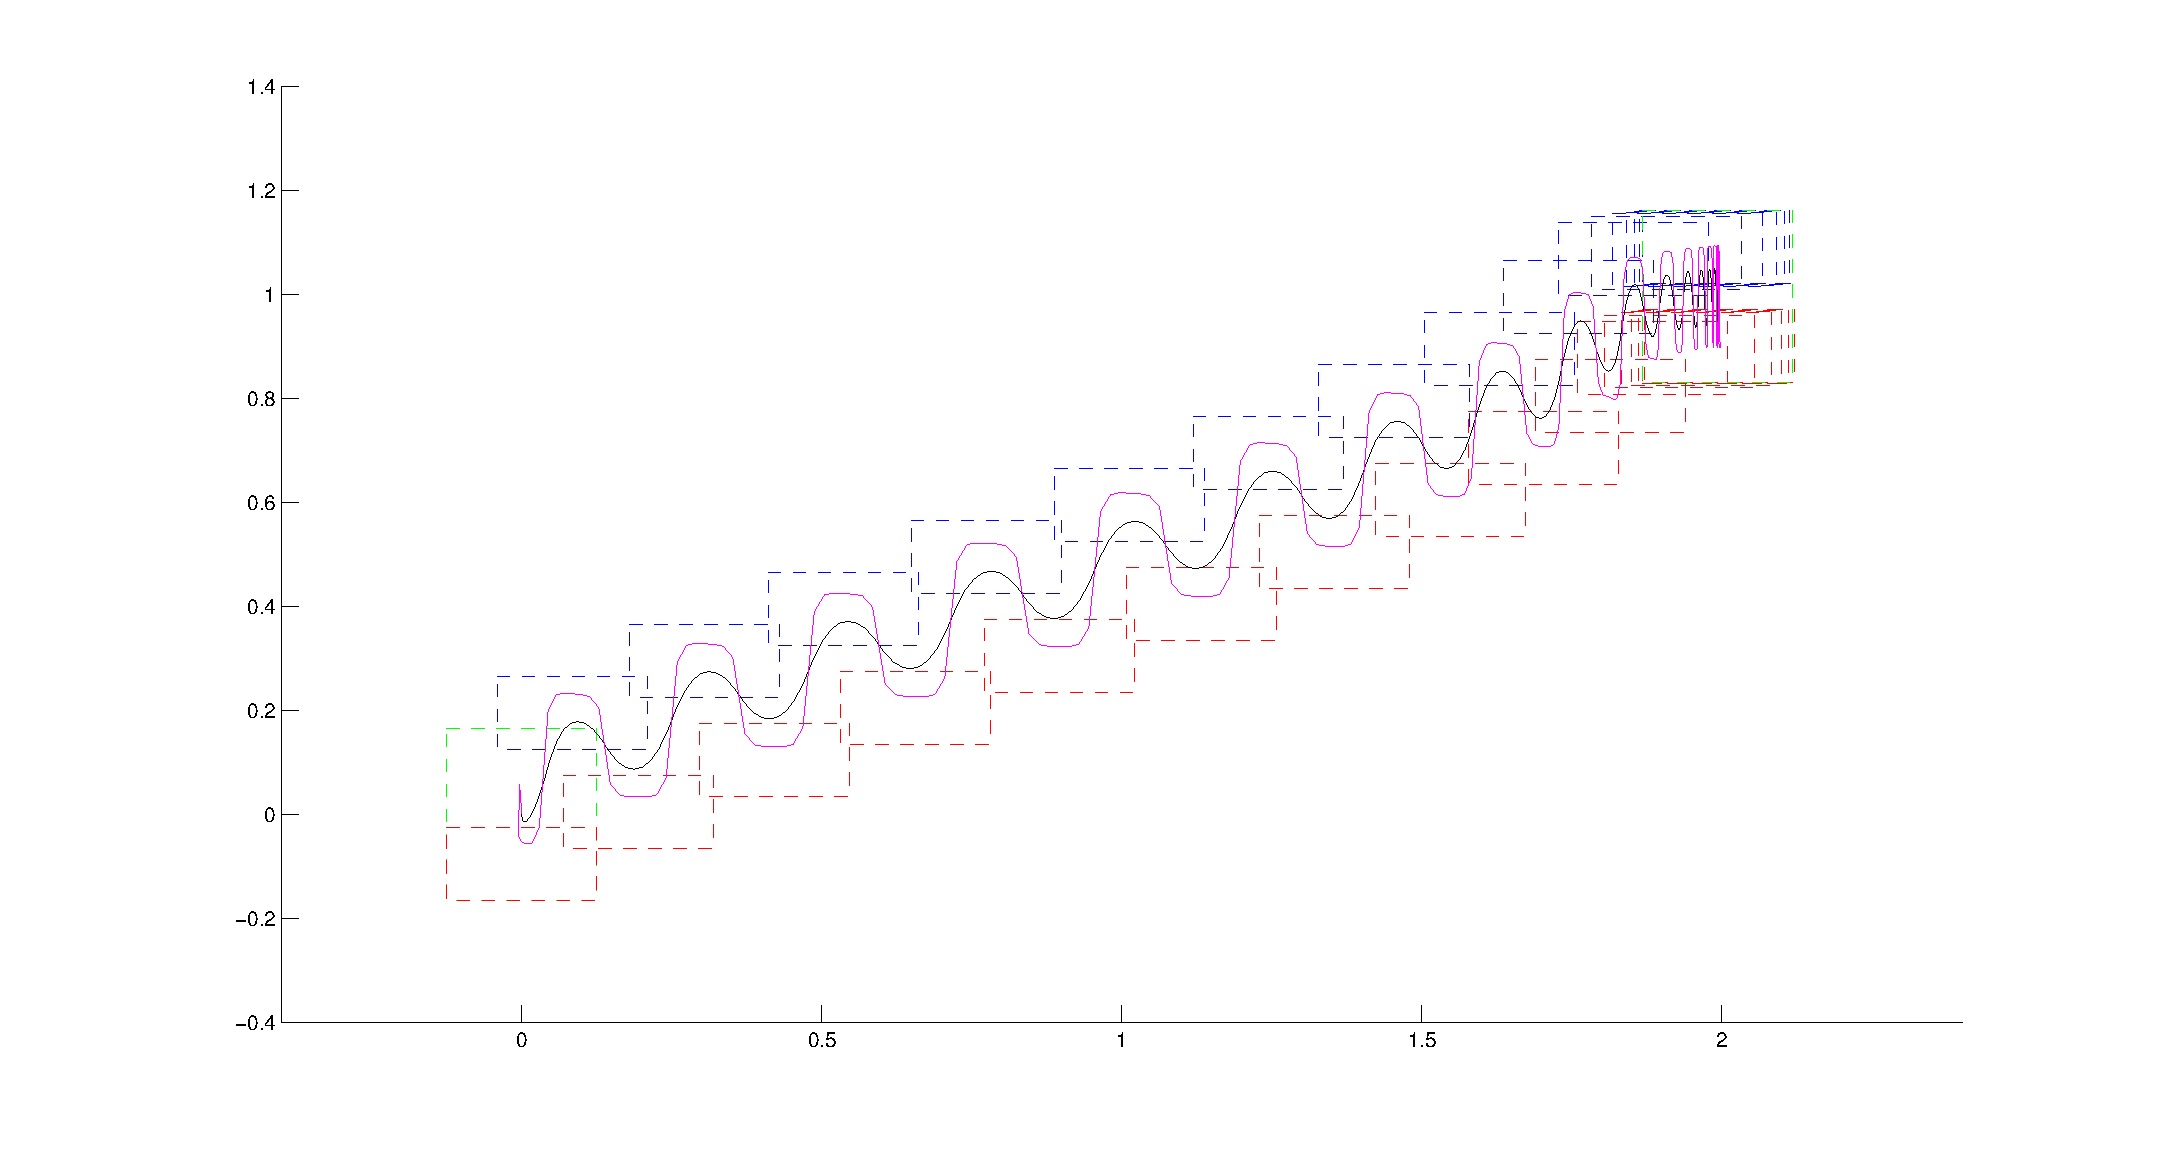
\includegraphics[scale=.25]{Chap4-Visual-Servoing/steps1_hrp2.pdf}
 %}
\end{minipage}
\begin{minipage}{0.5\textwidth}
 \centering
 %\subfigure[]{
 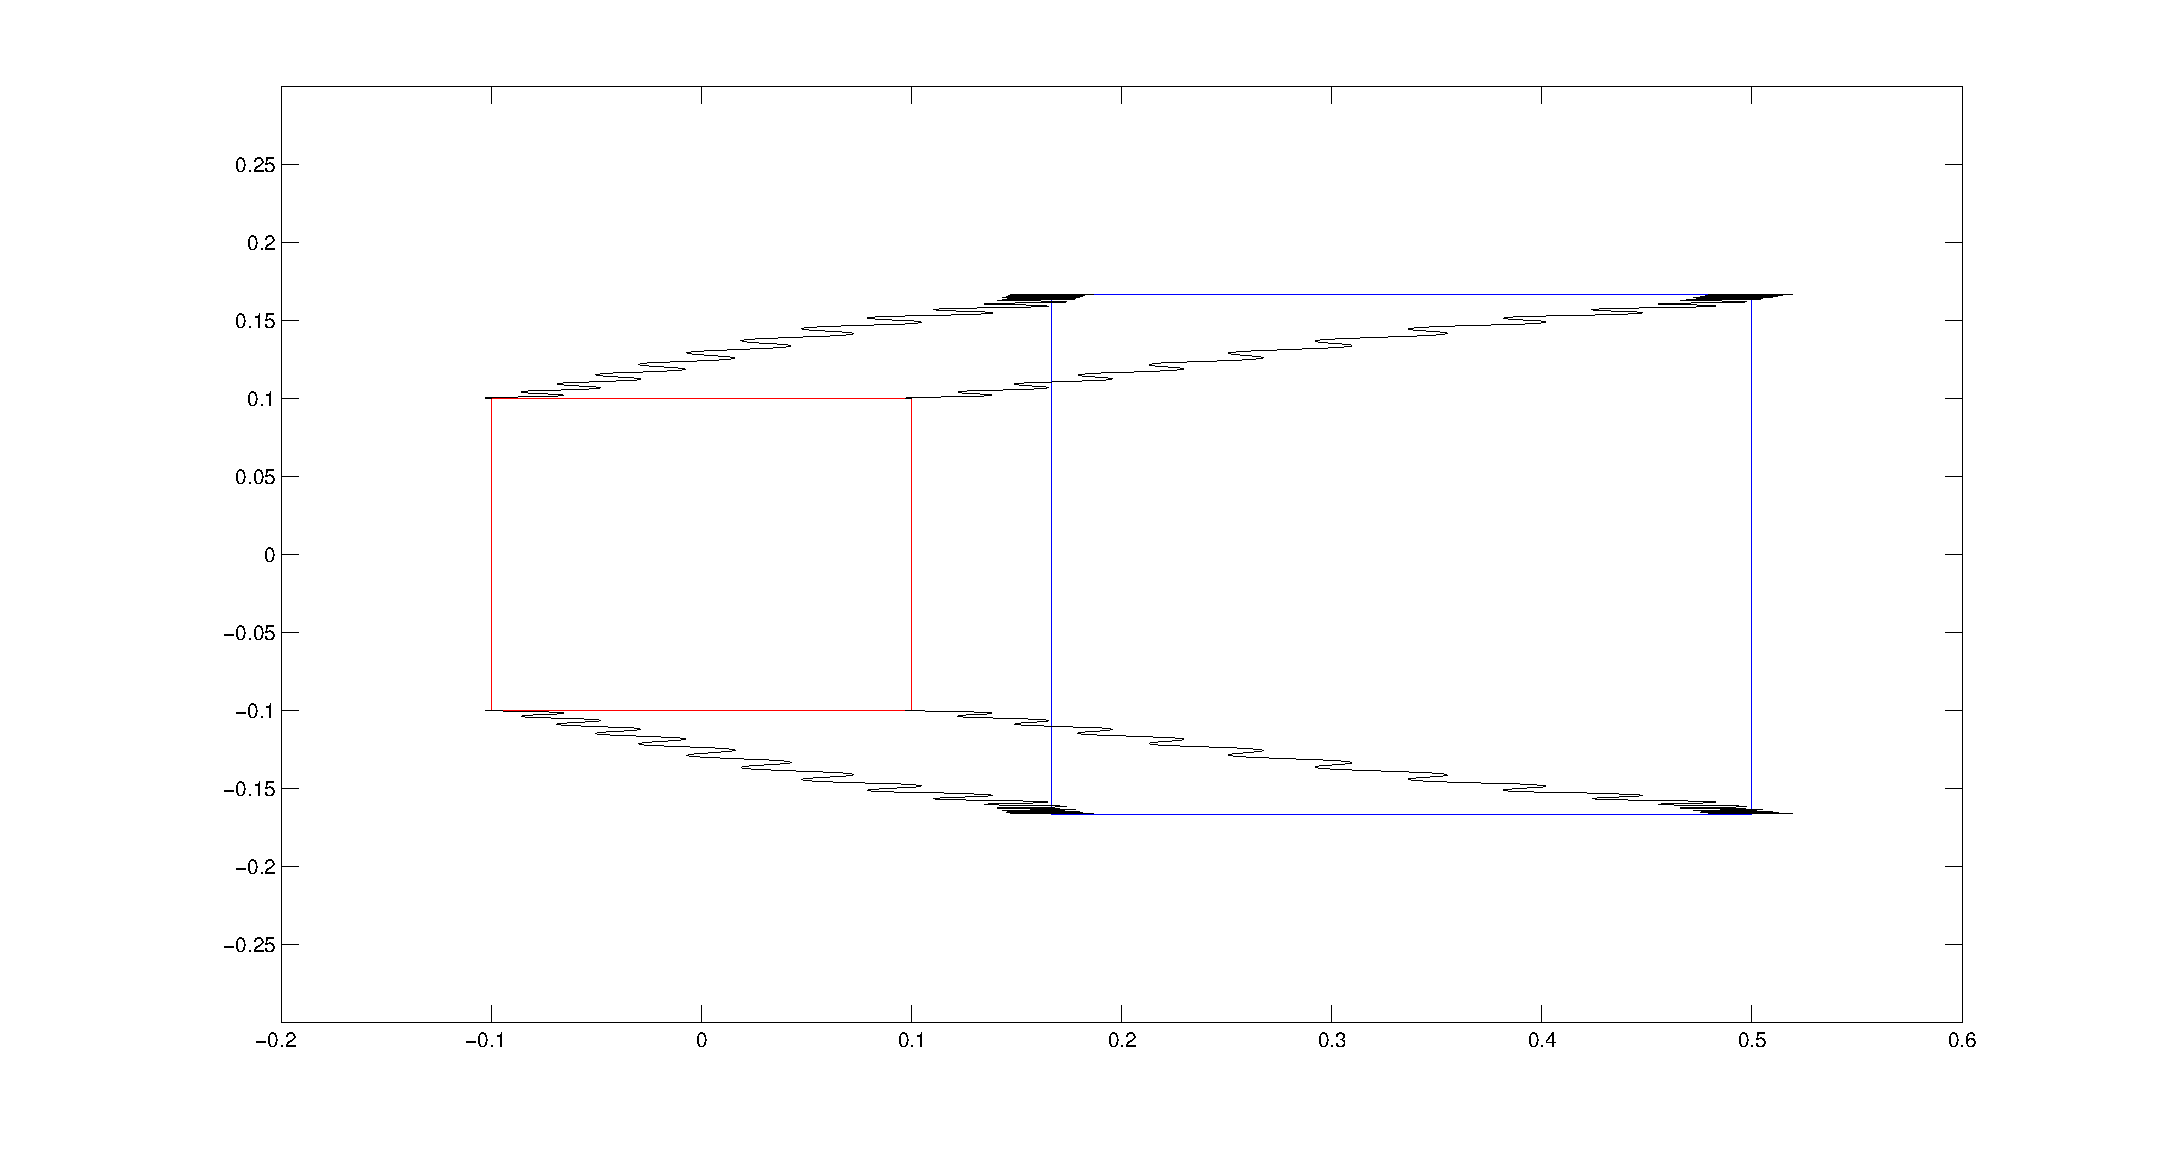
\includegraphics[width=5cm,height=4cm]{Chap4-Visual-Servoing/features1_hrp2.pdf}
 %}
\\
 %\subfigure[]{
 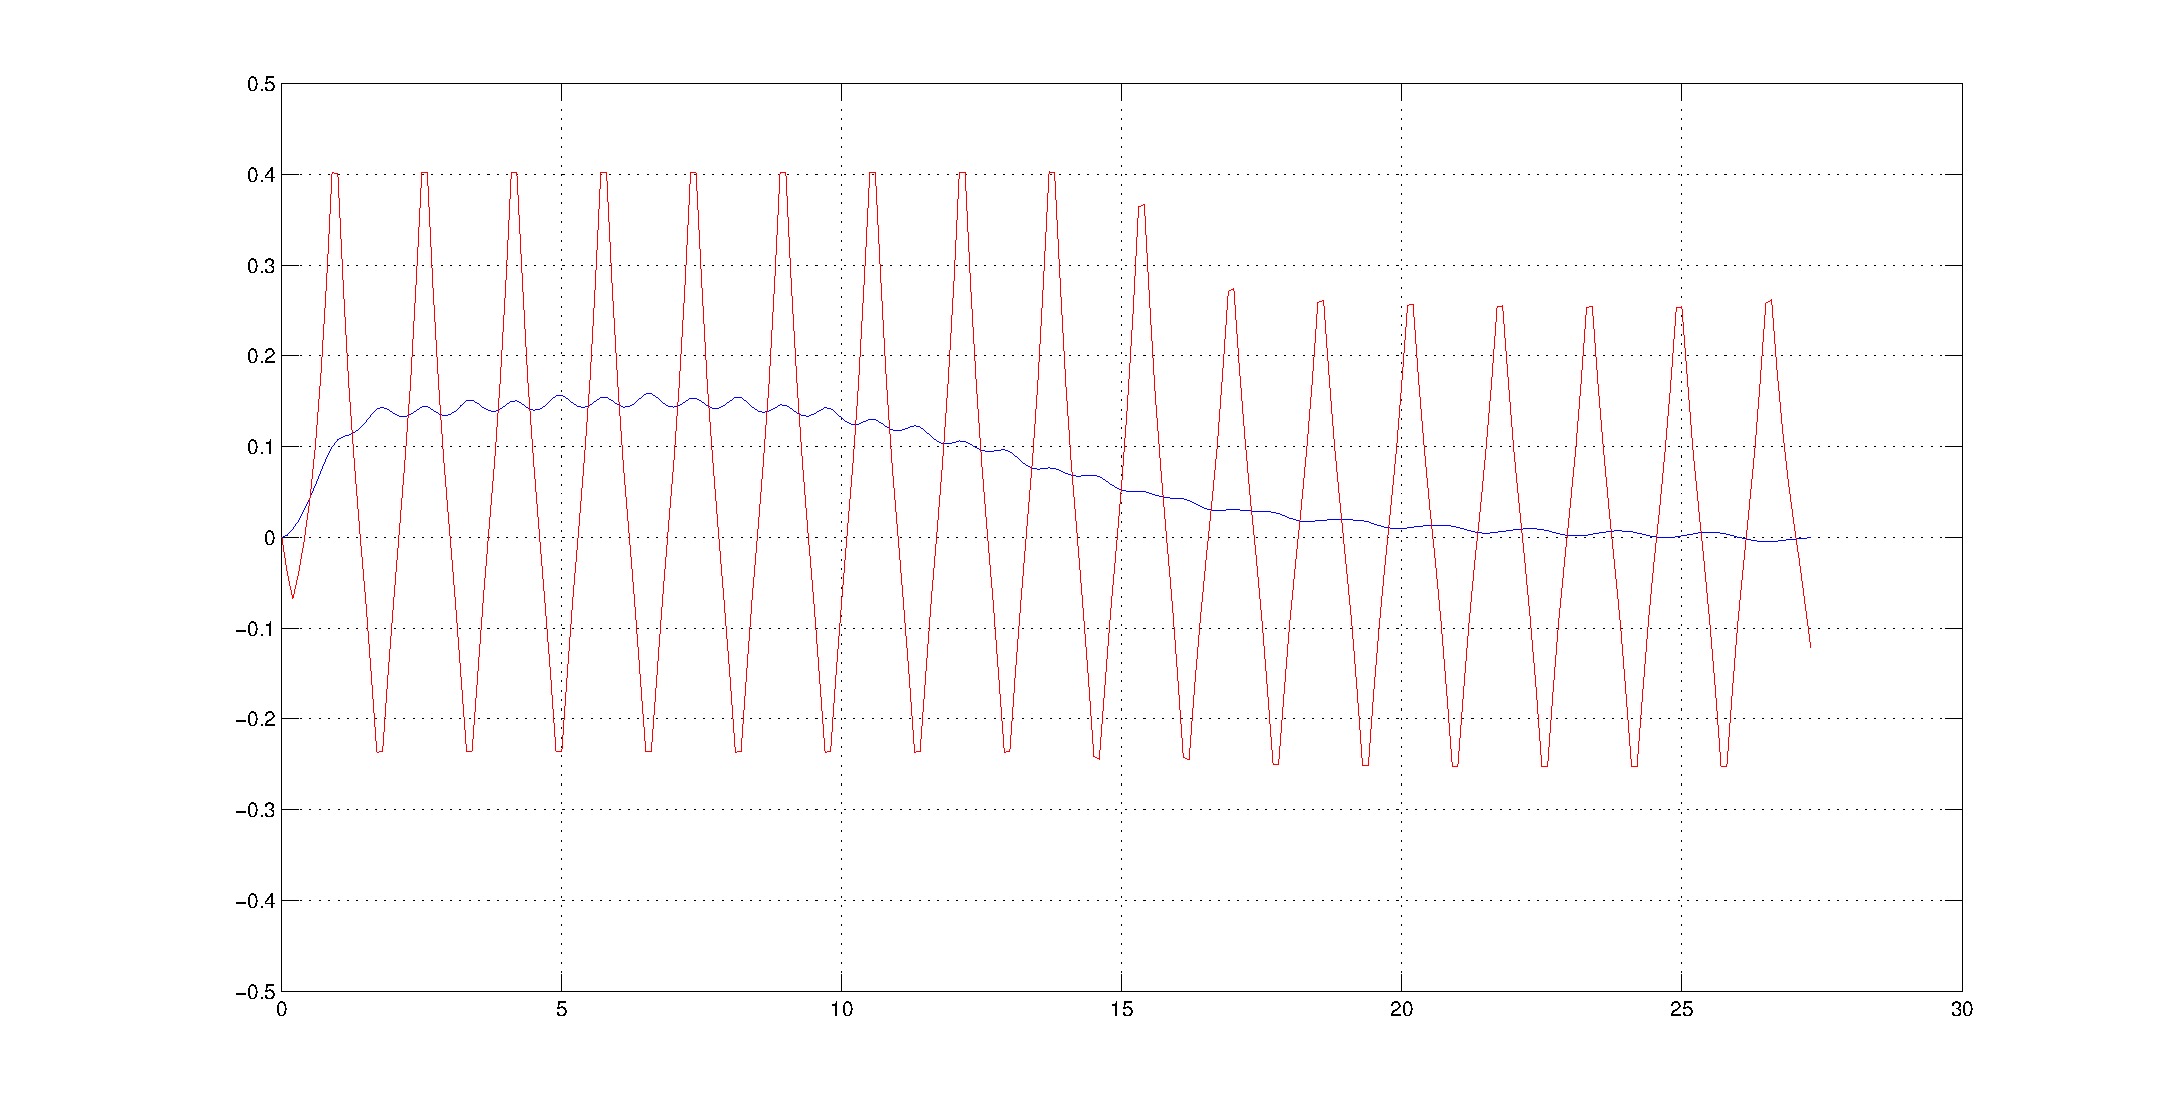
\includegraphics[scale=.2]{Chap4-Visual-Servoing/vels1_hrp2.pdf}
 %}
\end{minipage}
 \caption[]{\label{Fig:Results1}\small{On the left, we show the trajectory of the robot in the $x,y$ plane, driven by our MPC-based coupled approach. The initial and final double stance phases appear in green. The single stance support feet appear in red (resp. blue) for the right (resp. left) foot. In pink, we depicted the CoP trajectory, which can be observed to remain safely in the support polygon, and in black the CoM trajectory. On the right, top, we depict (in black) the trajectory of the features in the image, with the initial positions in red and the desired positions in blue, for the first simulation.  Finally, the evolution of the velocities is shown in the bottom. It is interesting to note the offset of the oscillatory velocity in $x$ (in blue) and $y$ (in red) due to the features errors.}}
 \end{figure*}


\begin{figure*}[h]
\begin{minipage}{0.5\textwidth}
 \centering
  %\subfigure[]{
 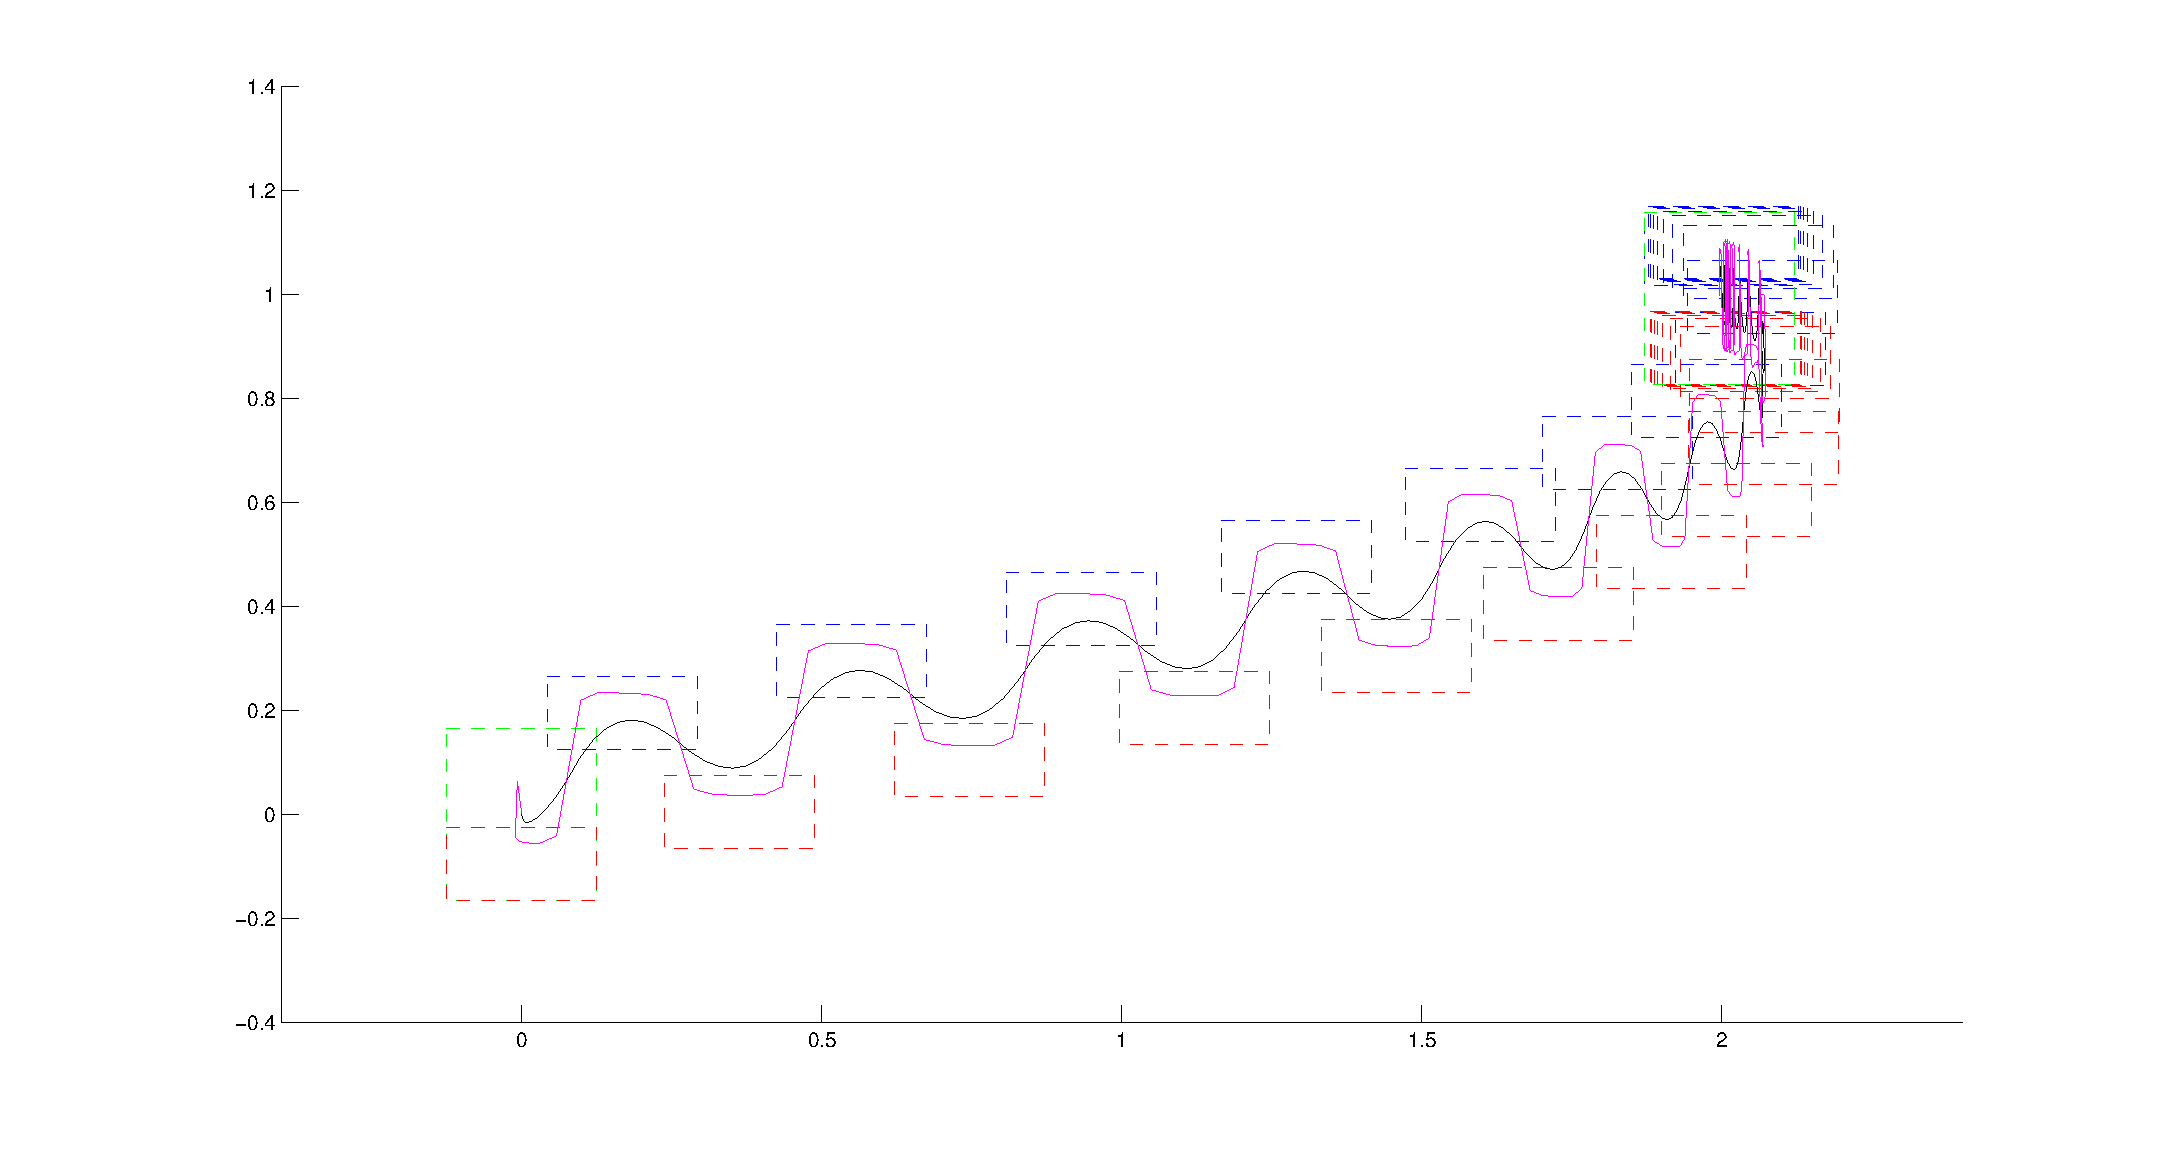
\includegraphics[scale=.25]{Chap4-Visual-Servoing/steps2_hrp2.pdf}
 %}
\end{minipage}
\begin{minipage}{0.5\textwidth}
 \centering
 %\subfigure[]{
 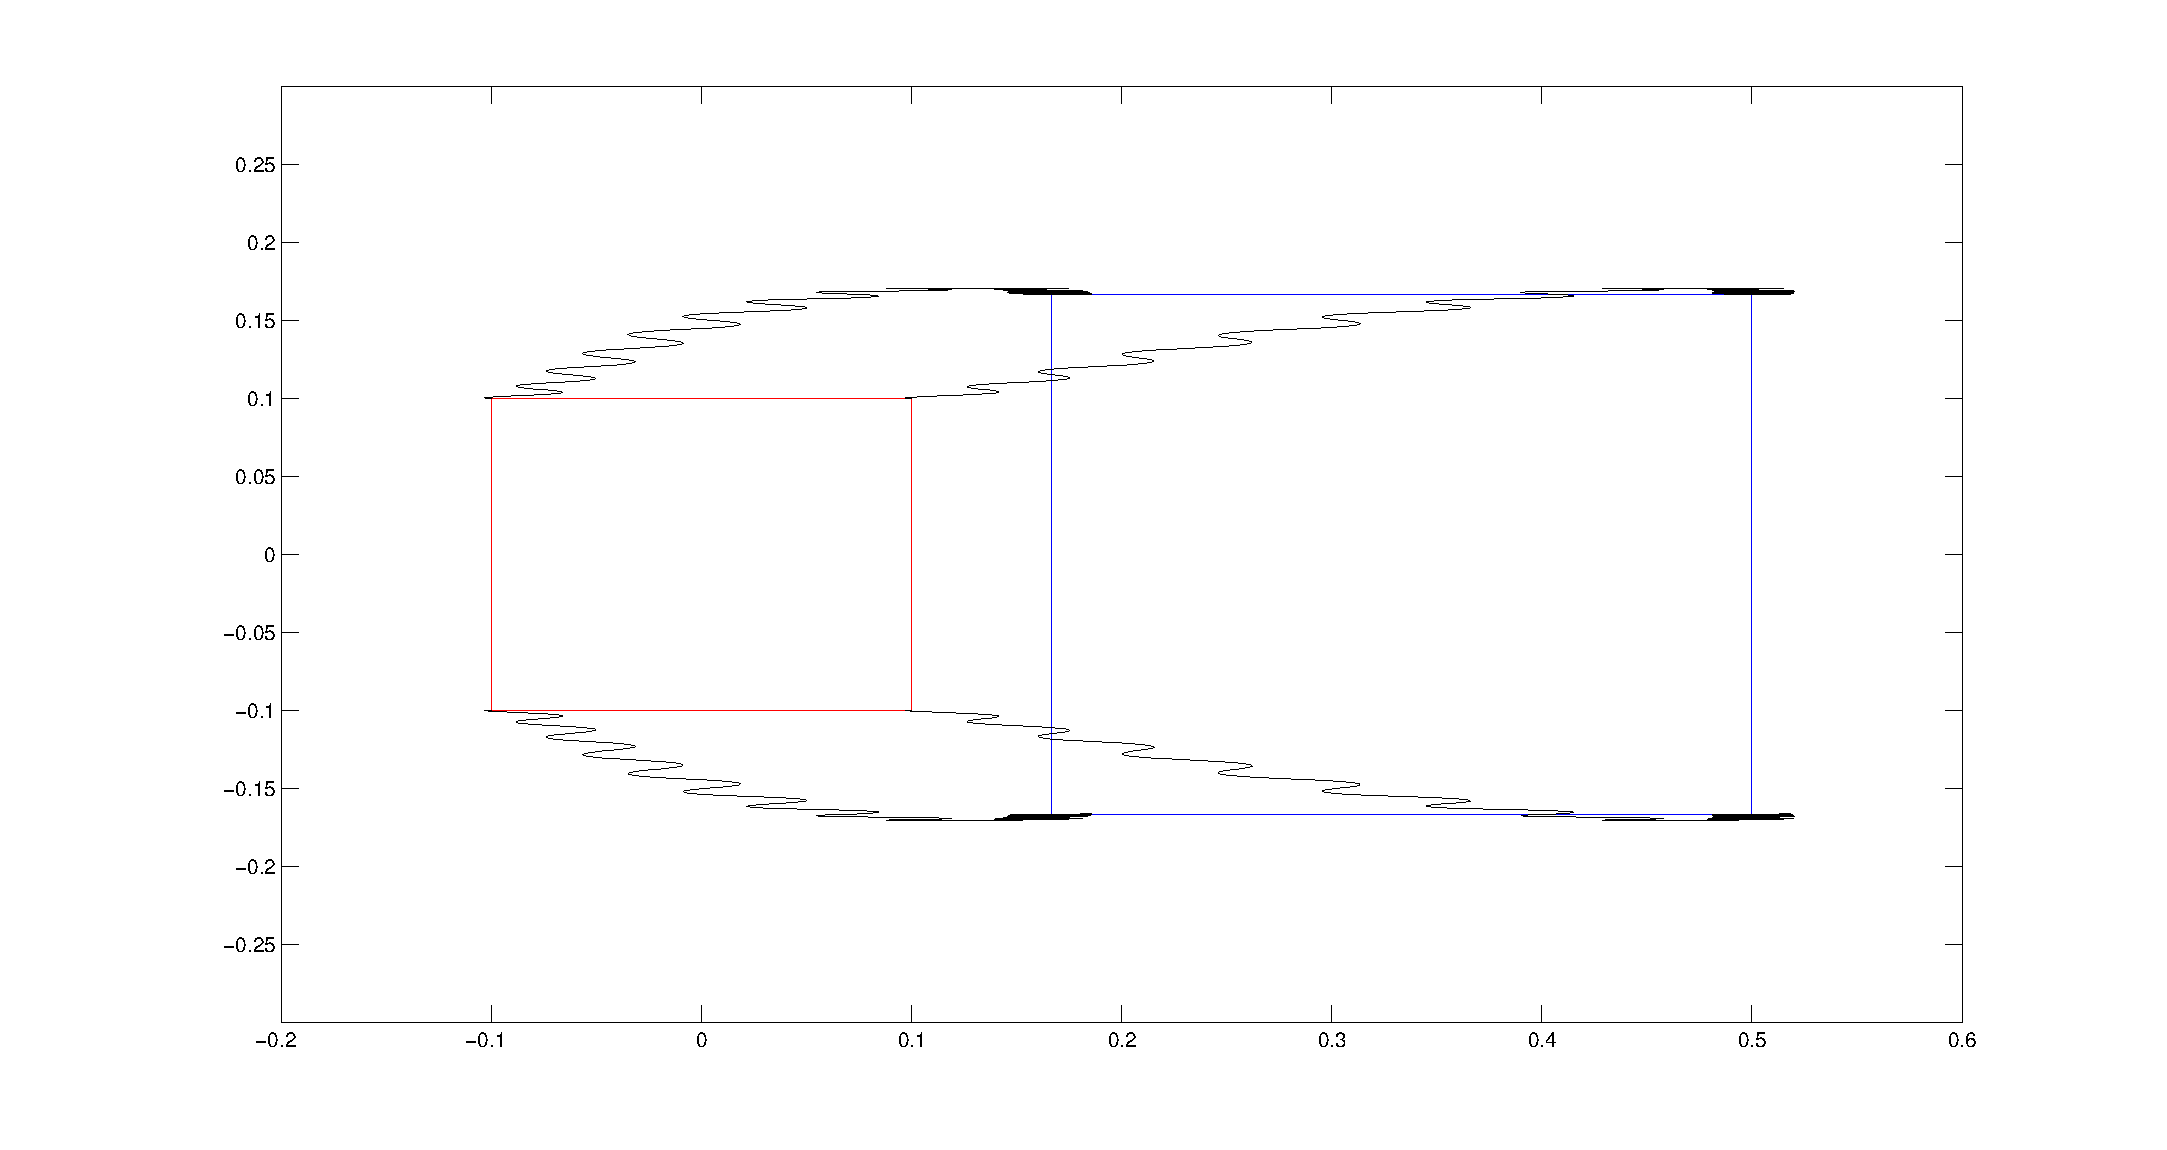
\includegraphics[width=5cm,height=4cm]{Chap4-Visual-Servoing/features2_hrp2.pdf}
 %}
\\
 %\subfigure[]{
 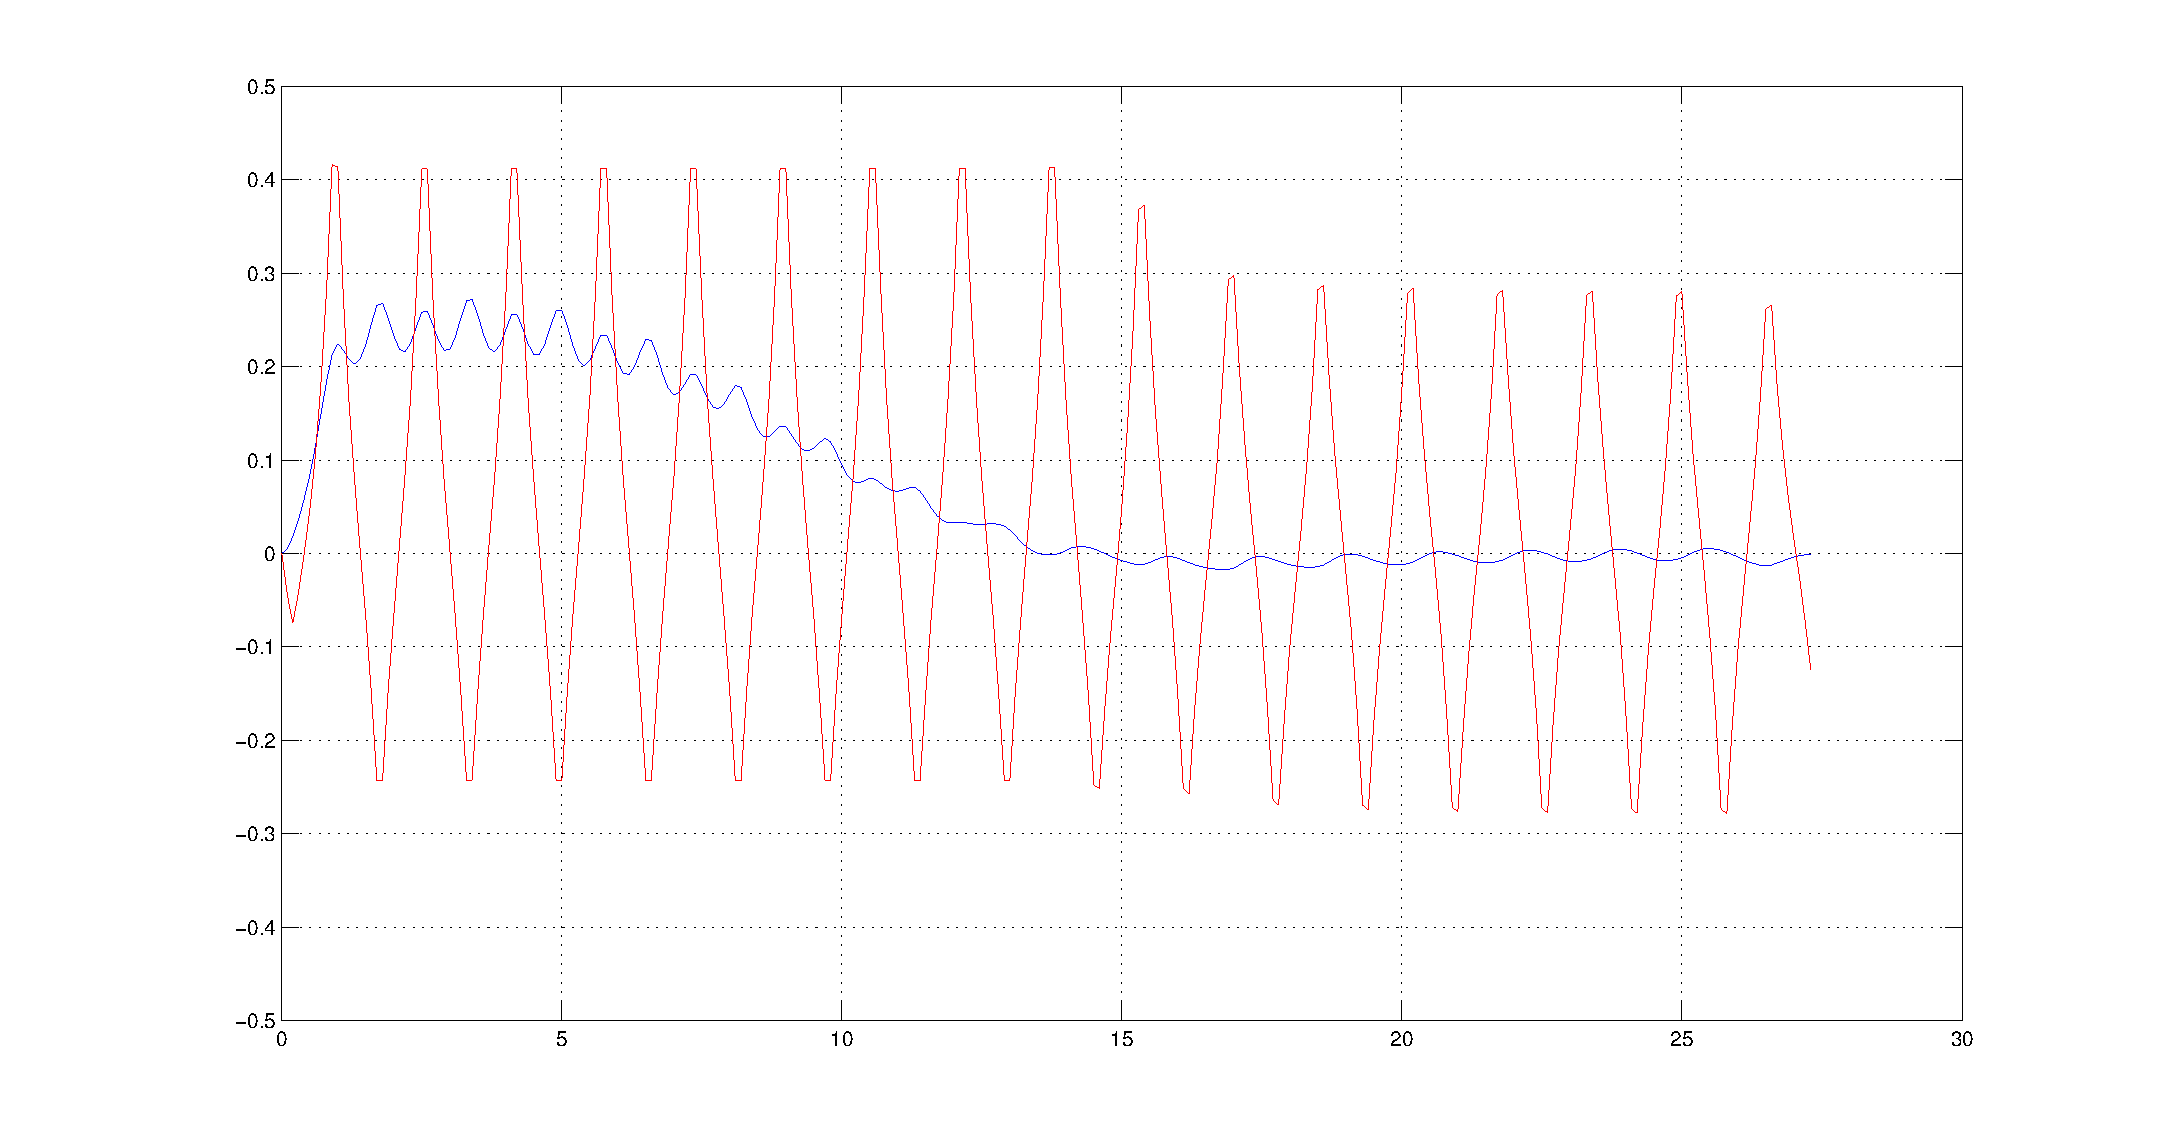
\includegraphics[scale=.2]{Chap4-Visual-Servoing/vels2_hrp2.pdf}
 %}
\end{minipage}
 \caption[]{\label{Fig:Results2}\small{The behavior of our system in the second simulation ($\beta$ is 5 times higher), with the same graphical conventions as in Fig.~\ref{Fig:Results1}. The robot is following a quite distinct trajectory, with a backwards part close to the end. As the priority is to minimize features errors, disregarding the jerks, high velocities are taken.}}
 \end{figure*}

Now, in a second experiment, we evaluate the trajectory with rotation. We recall that the rotation velocity control is decoupled from the $x$ and $y$ velocities control. It works as follows: The rotation velocity controller sets (in a decoupled way) the angular position while the main controller (QP) adapts the $x,y$ velocities in terms of these computed angular positions (which are known in the horizon), the visual errors, the footsteps centering and the jerks minimization. The results of a first simulation involving rotation is shown in Fig.~\ref{Fig:Results3}. One can observe that the dynamical balance is kept, and that most of the correction related to the rotation is done at the beginning of the trajectory. Also, in Fig.~\ref{Fig:Results4}, we can see that it is robust to perturbations: The same trajectory is followed as in Fig.~\ref{Fig:Results3} but a strong perturbation in the CoM position has been introduced (simulating an external force applying to the CoM or a string error in the position estimation), inducing visible peaks in the velocities. However, the perturbation is recovered quasi-instantly.

\begin{figure*}[h]
\begin{minipage}{0.5\textwidth}
 \centering
  %\subfigure[]{
 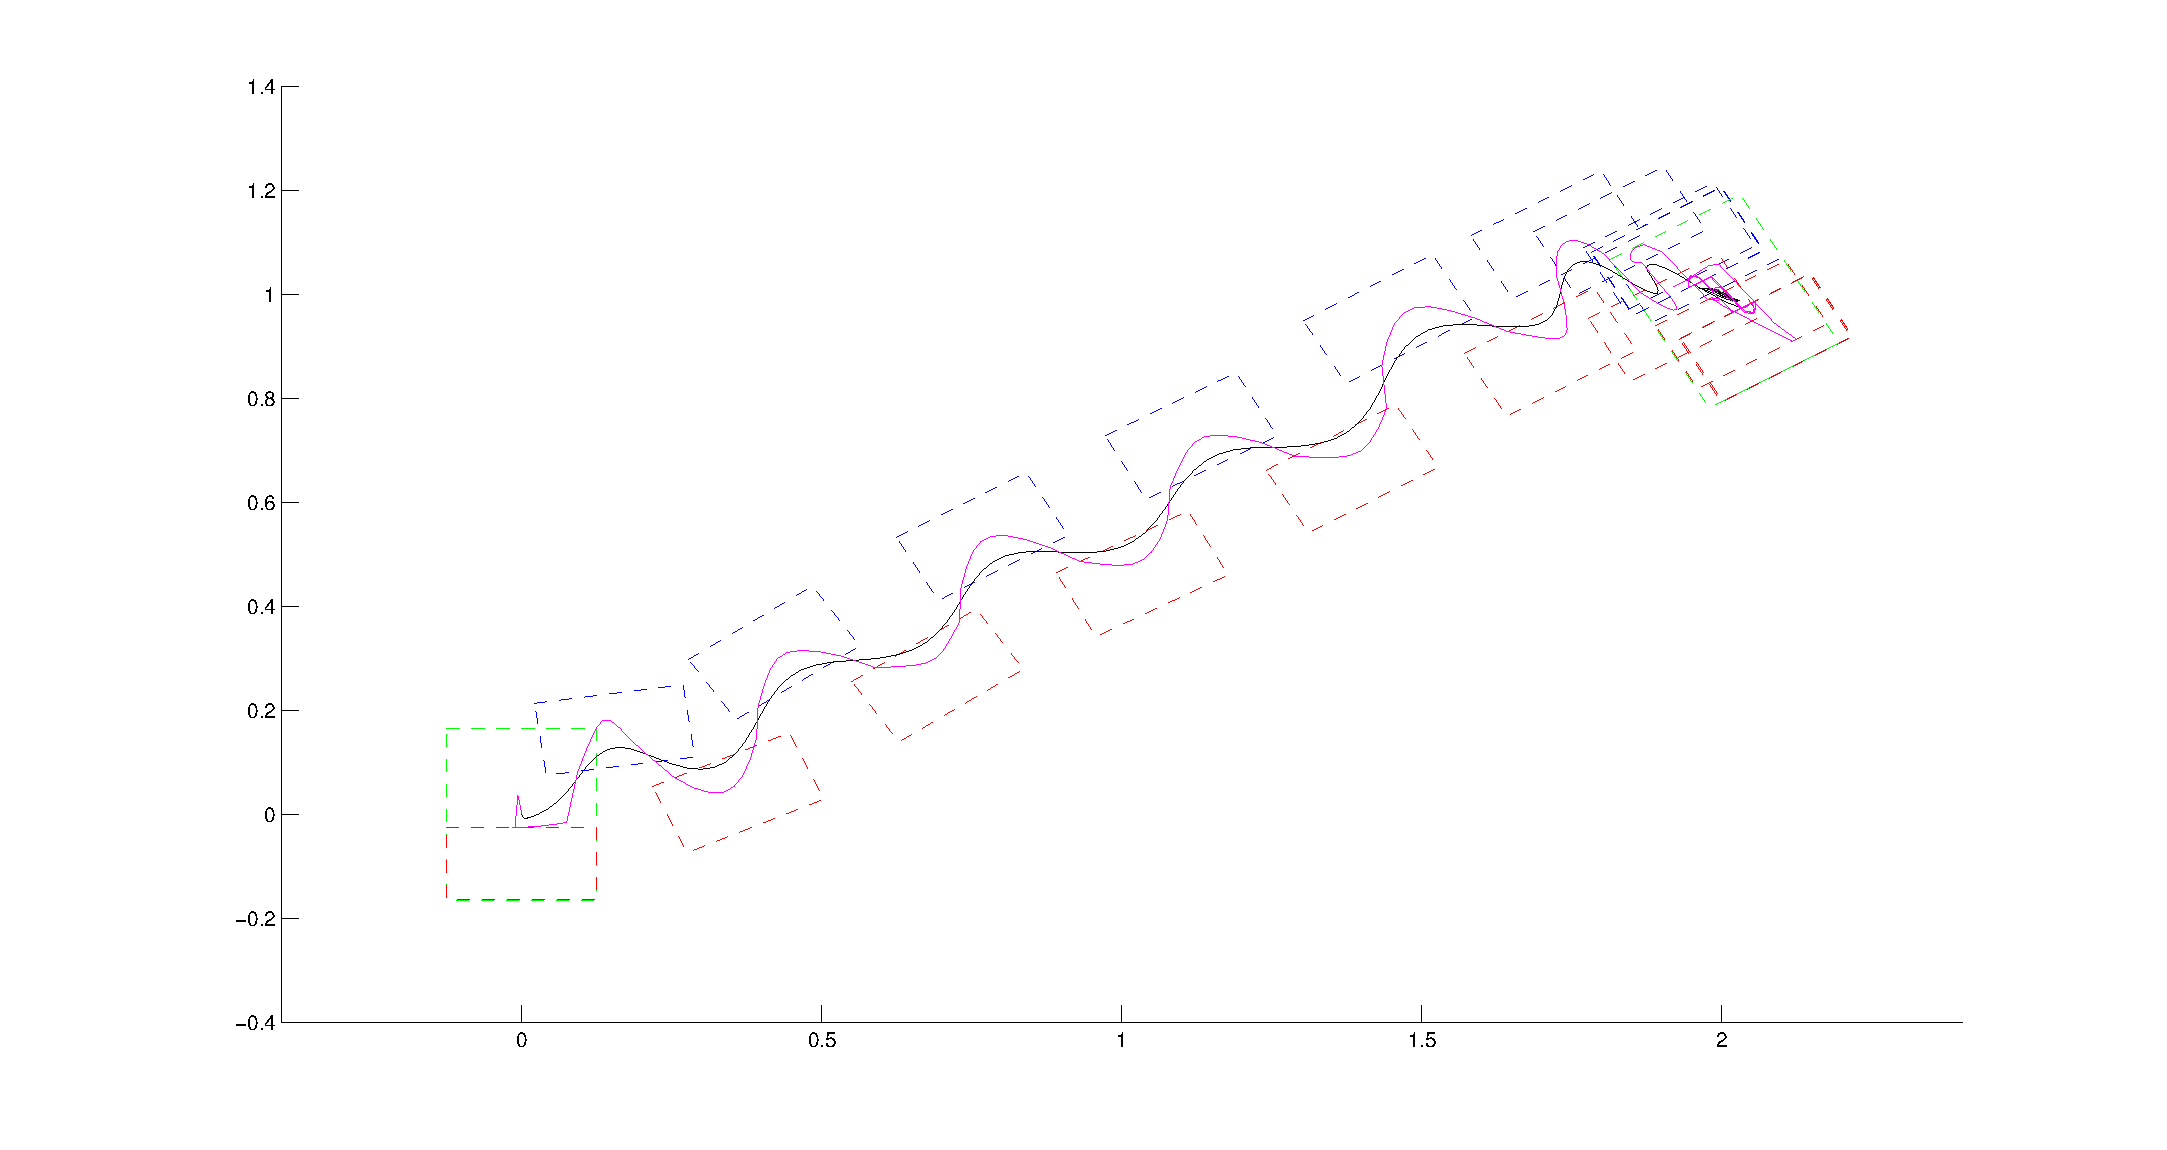
\includegraphics[scale=.25]{Chap4-Visual-Servoing/steps3_hrp2.pdf}
 %}
\end{minipage}
\begin{minipage}{0.5\textwidth}
 \centering
 %\subfigure[]{
 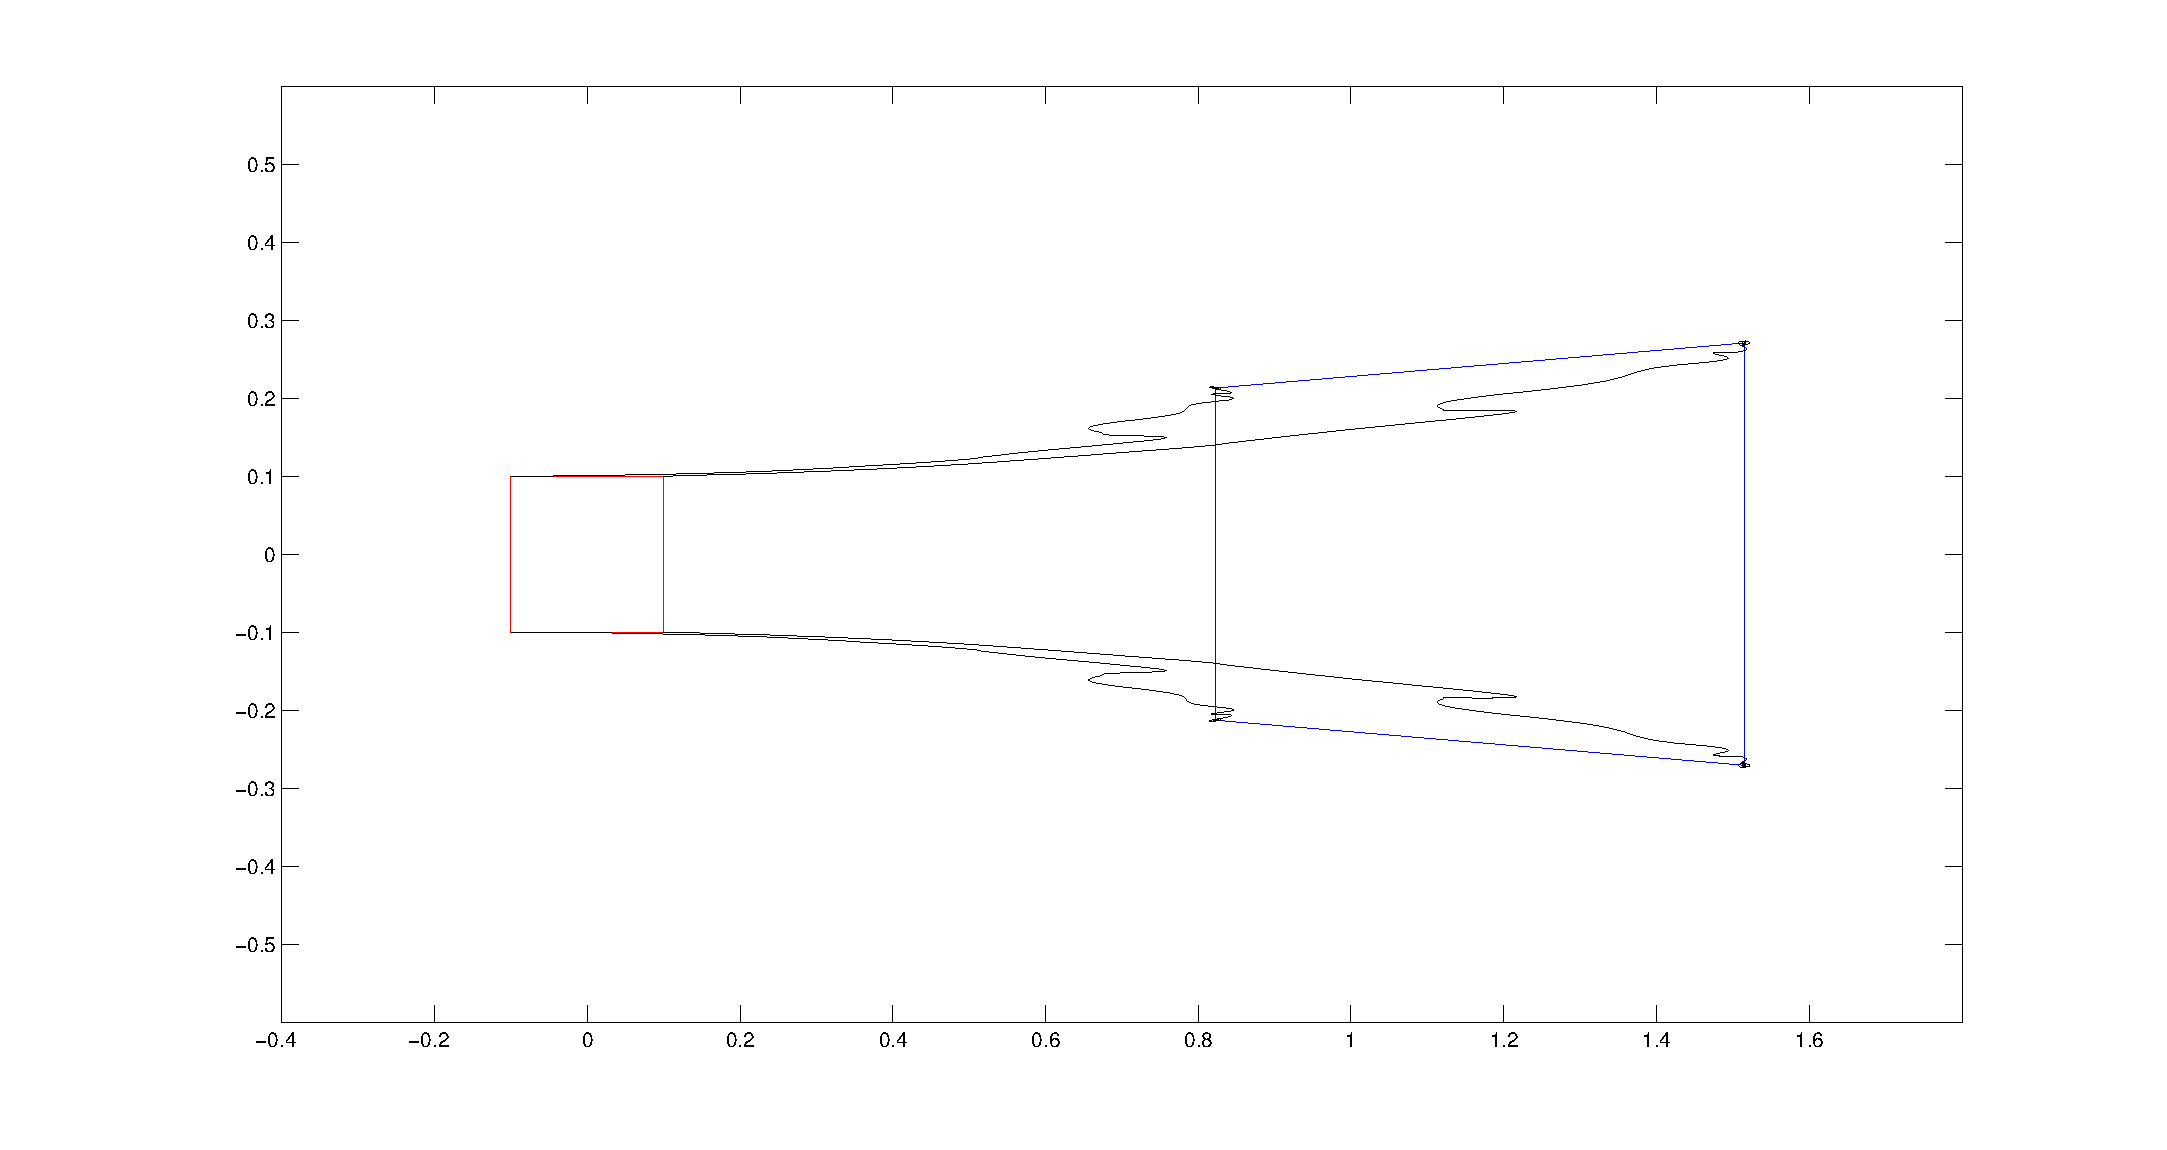
\includegraphics[width=5cm,height=4cm]{Chap4-Visual-Servoing/features3_hrp2.pdf}
 %}
\\
 %\subfigure[]{
 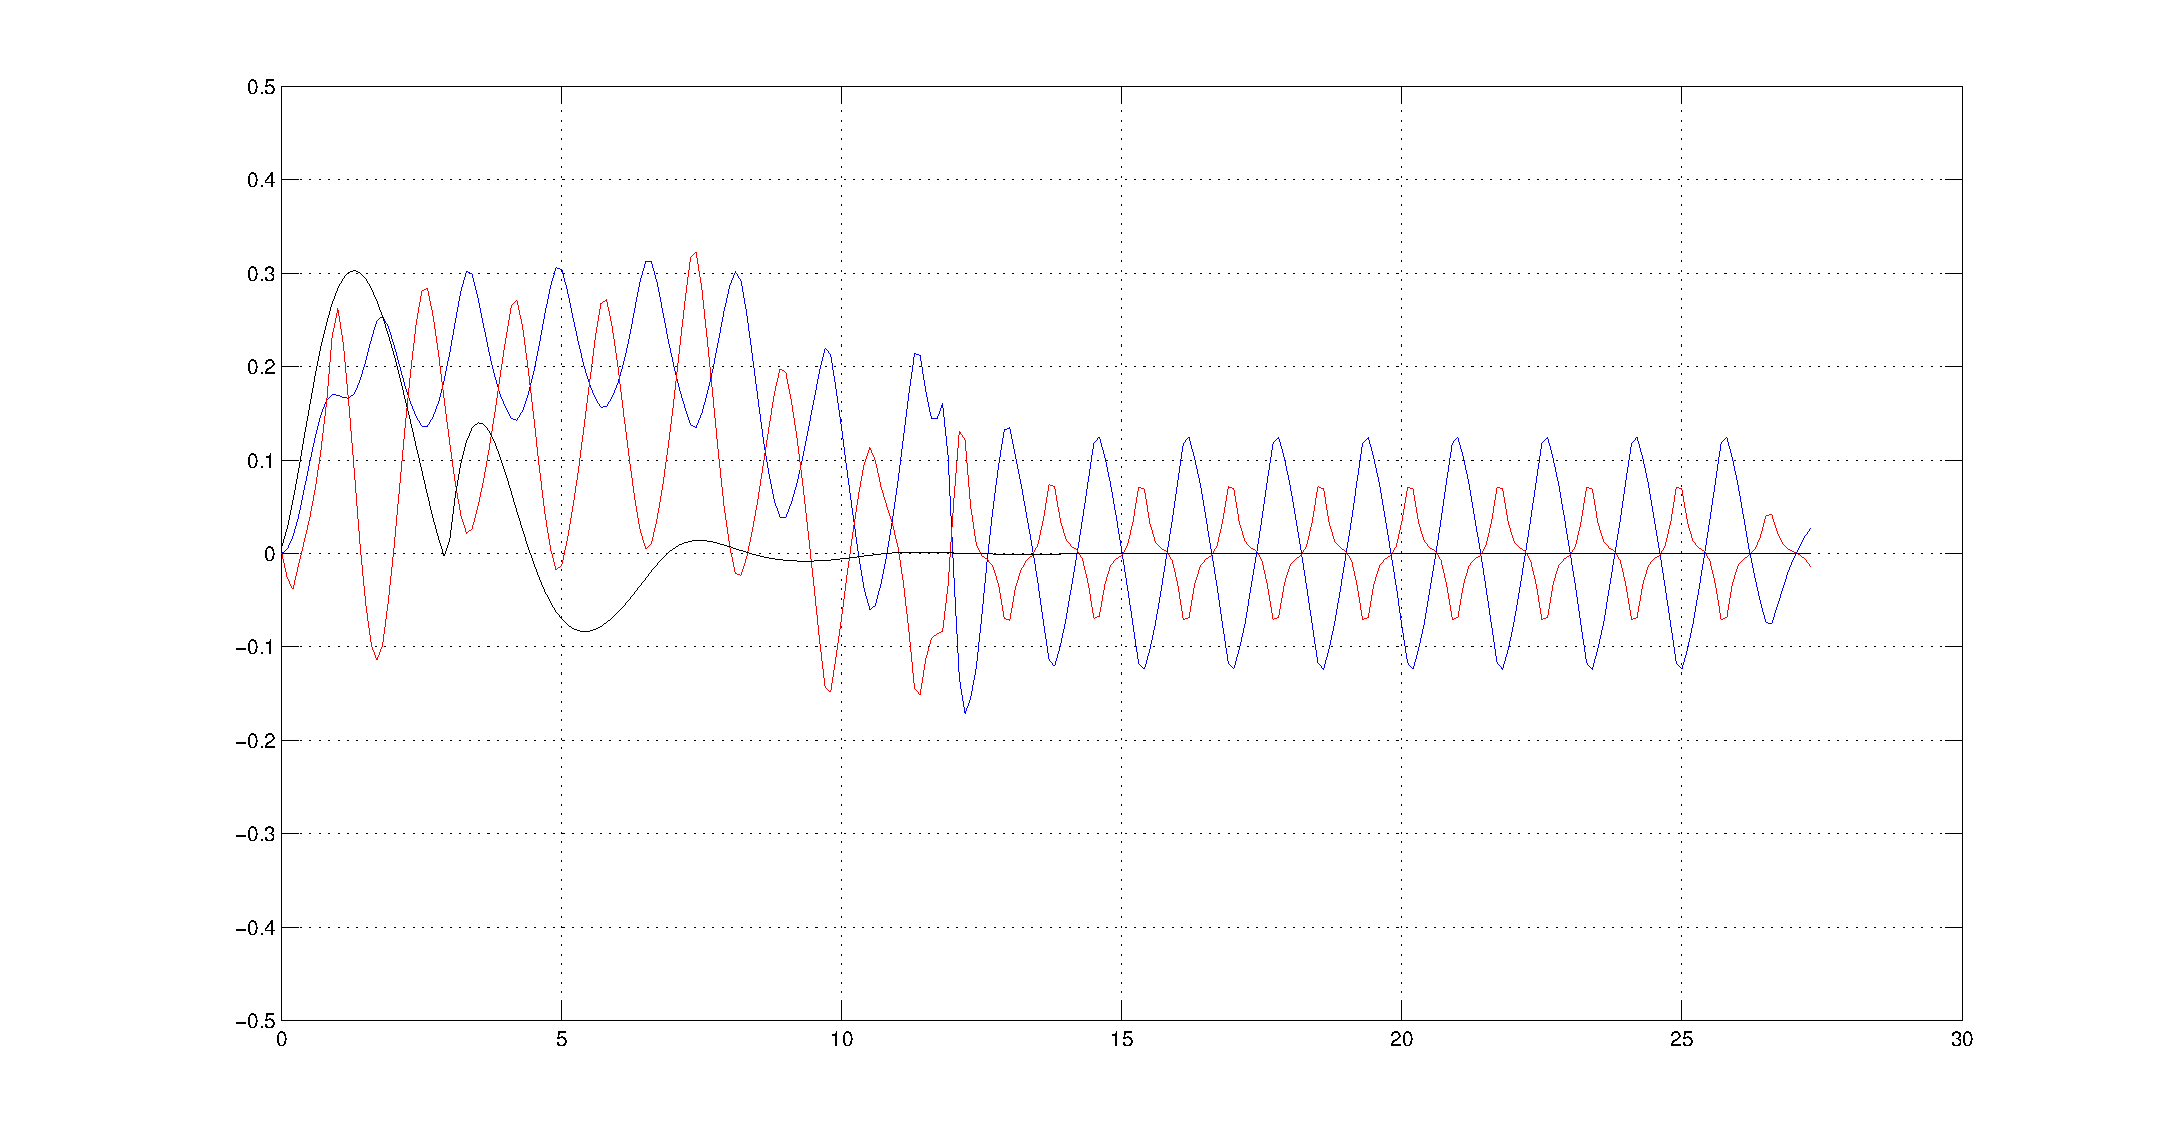
\includegraphics[scale=.2]{Chap4-Visual-Servoing/vels3_hrp2.pdf}
 %}
\end{minipage}
 \caption[]{\label{Fig:Results3}\small{The behavior of our system in the third simulation, involving rotation, with the same graphical conventions as in Fig.~\ref{Fig:Results1}. In the velocities graph (right, bottom) we added the rotation velocity in black. The robot is walking in the sagittal direction most of the time, after an initial rotation. The amplitude of the oscillations of the CoM and subsequently of the features are smaller than in the first simulation. However, we can see a non-negligible component of velocity in the positive $y$ direction, since the angle is not fully compensated. When the angle is almost fully compensated, this component disappears.}}
 \end{figure*}

\begin{figure*}[h]
\begin{minipage}{0.5\textwidth}
 \centering
  %\subfigure[]{
 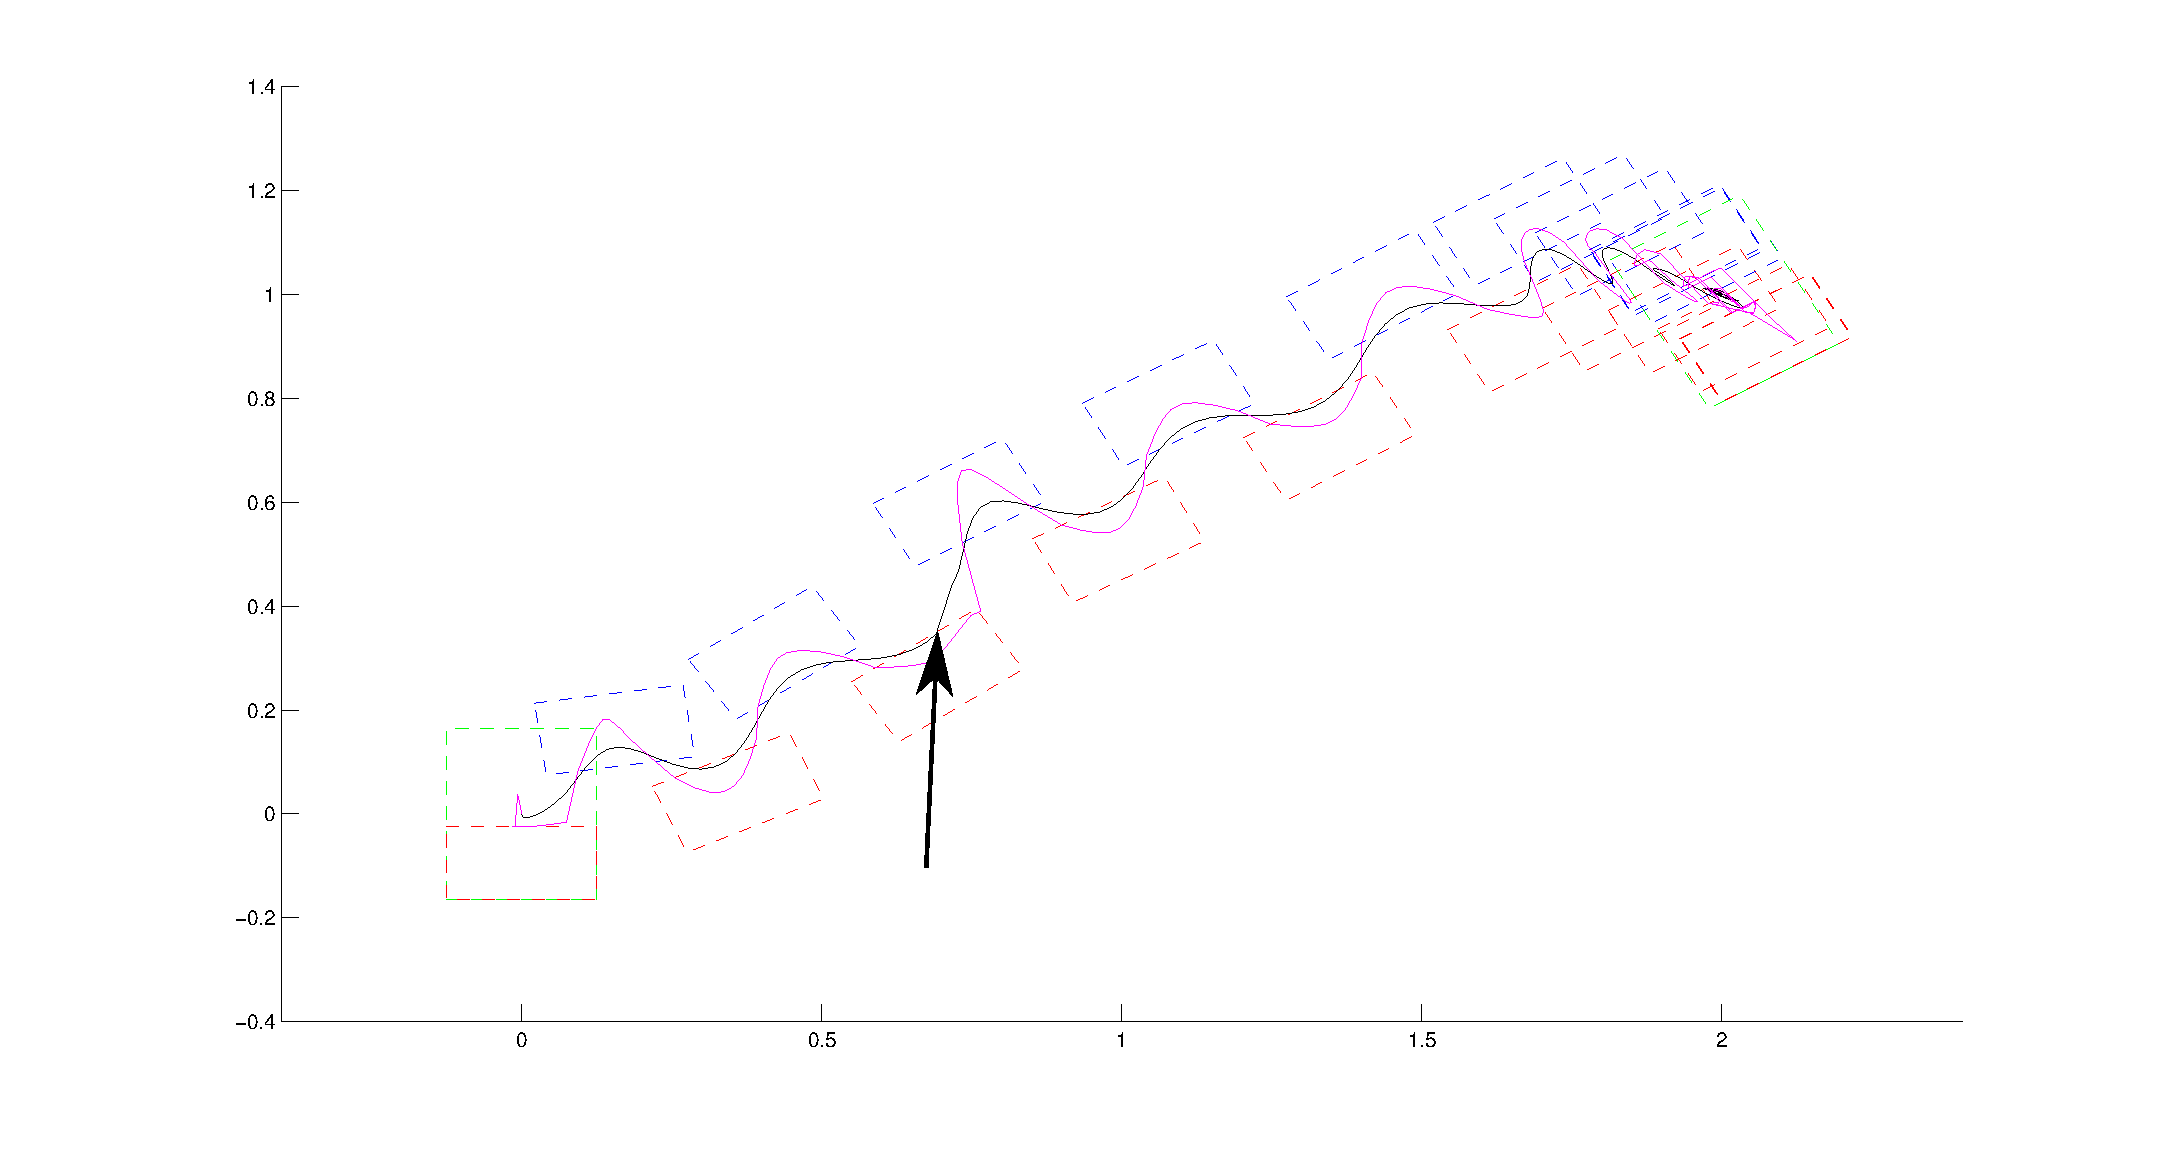
\includegraphics[scale=.25]{Chap4-Visual-Servoing/steps4_hrp2_1.pdf}
 %}
\end{minipage}
\begin{minipage}{0.5\textwidth}
 \centering
%\subfigure[]{
 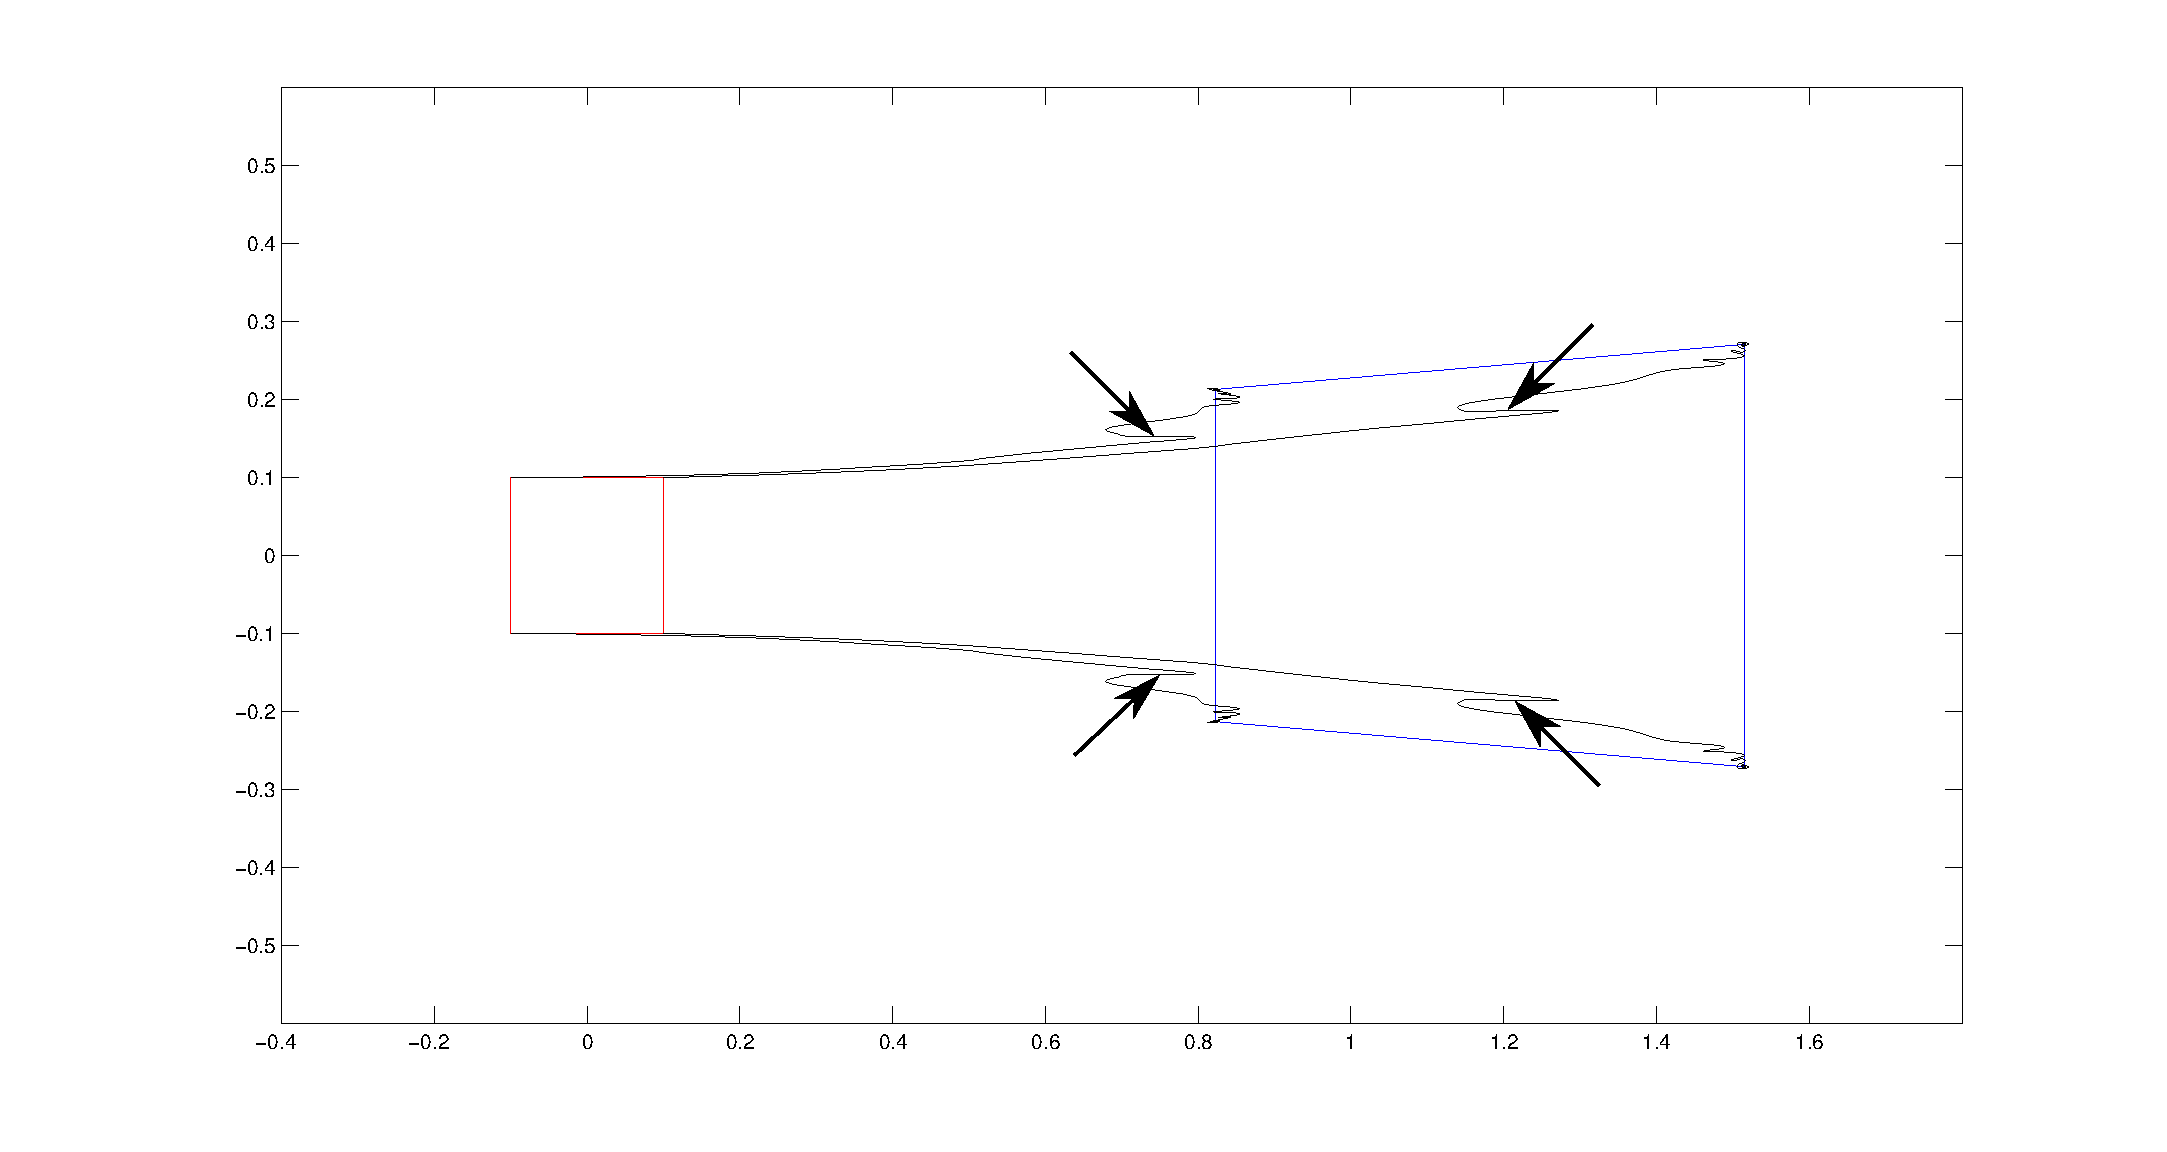
\includegraphics[width=5cm,height=4cm]{Chap4-Visual-Servoing/features4_hrp2_1.pdf}
 %}
\\
 %\subfigure[]{
 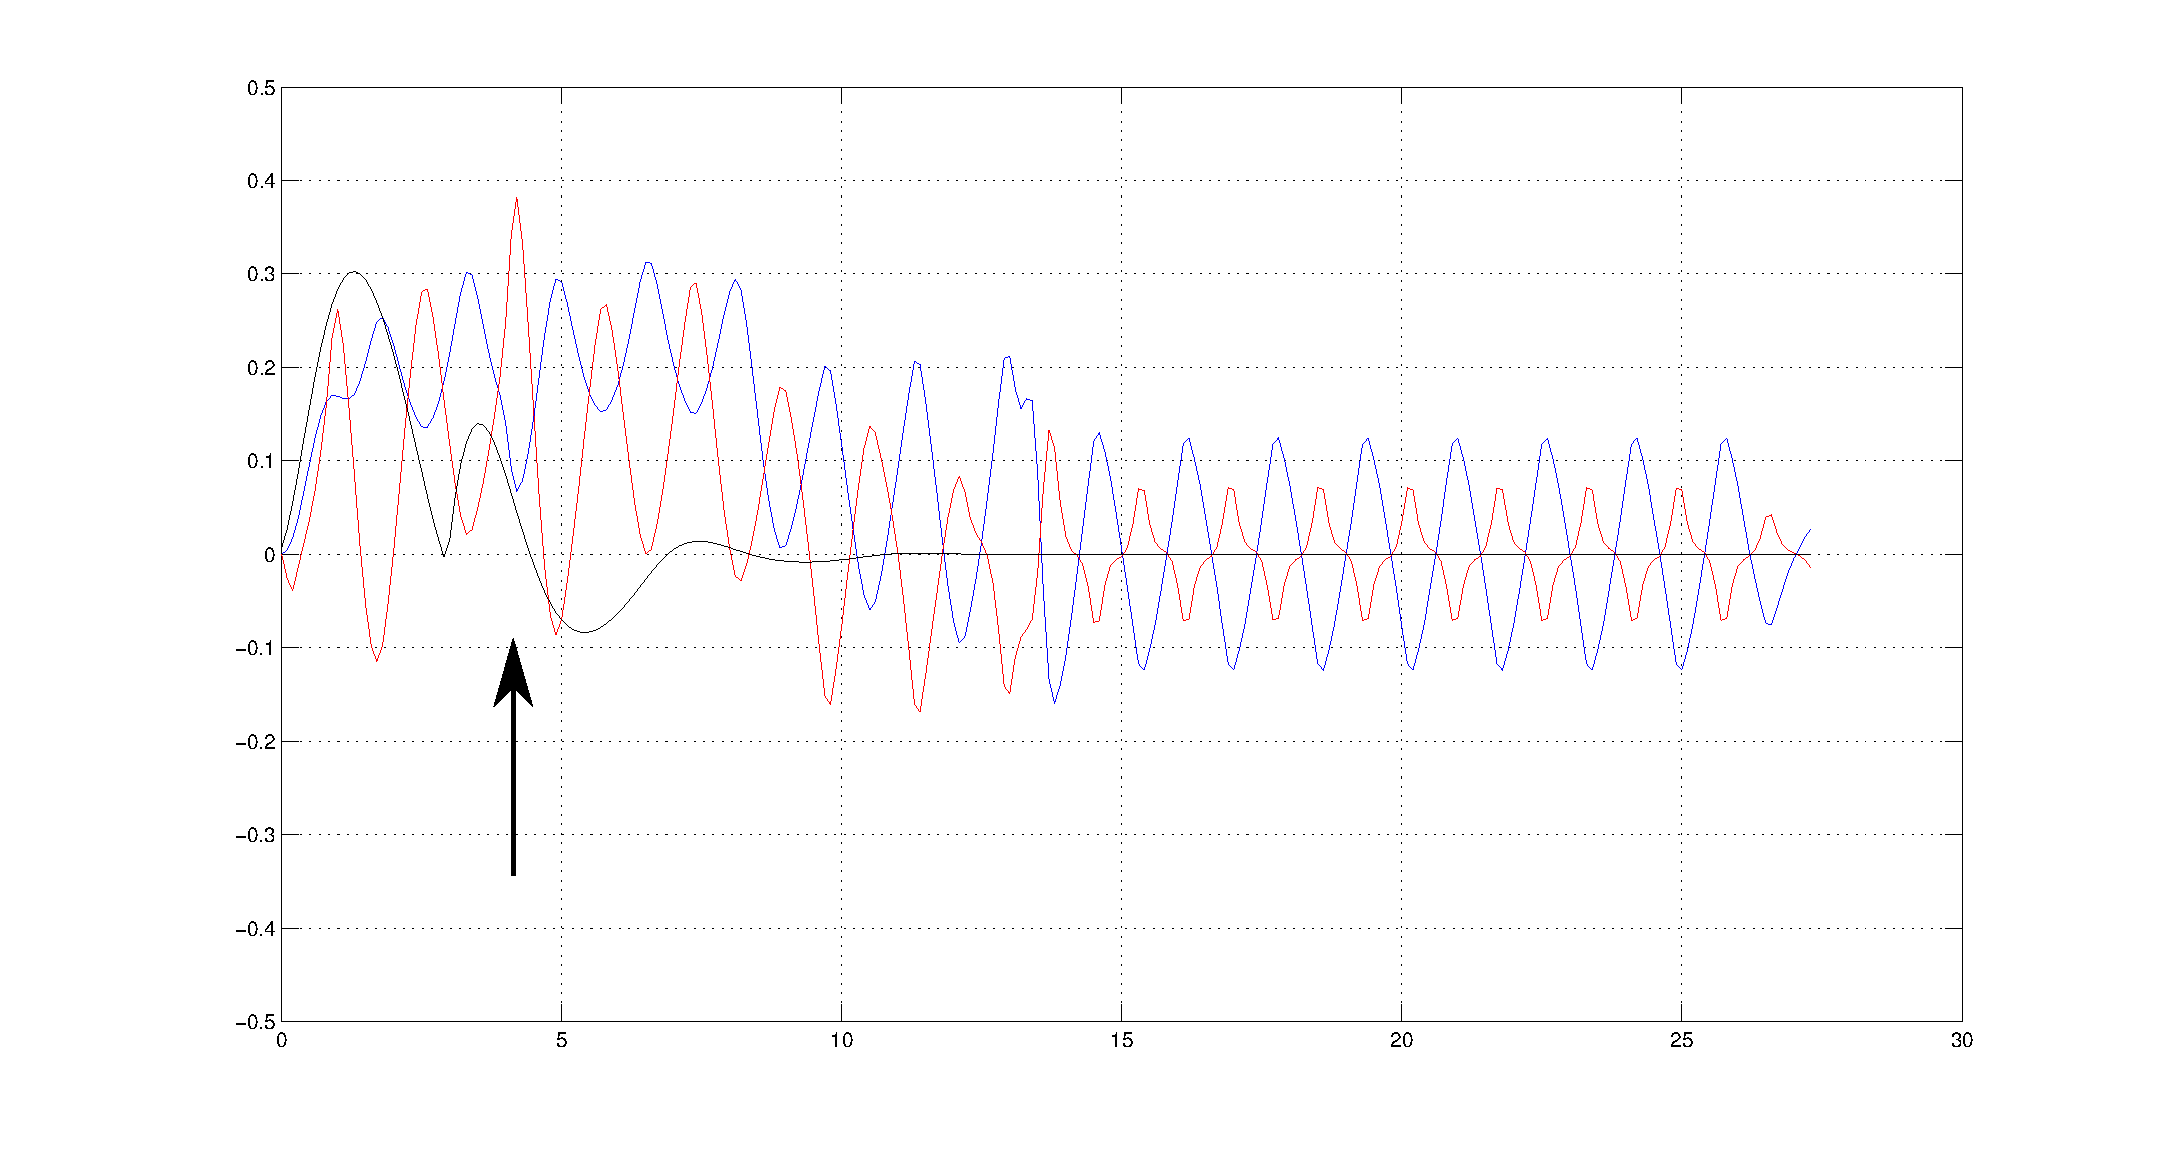
\includegraphics[scale=.2]{Chap4-Visual-Servoing/vels4_hrp2_1.pdf}
 %}
\end{minipage}
 \caption[]{\label{Fig:Results4}\small{The behavior of our system in the fourth simulation, with the same graphical conventions as in Fig.~\ref{Fig:Results3}. The robot is following a trajectory similar to the one of Fig.~\ref{Fig:Results3}. After a few footsteps, a strong perturbation is applied to the CoM, inducing a peak in the velocities graph (right, bottom). This perturbation is small in distance metric, so it is not visible in the features trajectories. The perturbation is quasi-instantly recovered.}}
 \end{figure*}

We have already explained how a local linearization is made to maintain the QP formulation. The performance of this linearization depends of the distance traveled inside the horizon, which depends on the velocity of the robot and the size of the horizon. In Fig.~\ref{Fig:Results5}, we can see the linearized and real features trajectories for a given CoM trajectory. As expected, close to the beginning (the linearization point) the trajectories are quite similar, while the final positions differ more. This is an extreme situation, since usual metric displacements in the horizon are much smaller than this one. In any case, horizon displacements are bigger when the visual errors are bigger (the robot is far from the desired position) in which case the robot just needs a tendency. But when the errors are getting smaller, the robot needs more precision. In this case, the displacements in the horizon becomes smaller so that the difference between the real model and the linearized one becomes negligible.

\begin{figure}[h]
 \centering
 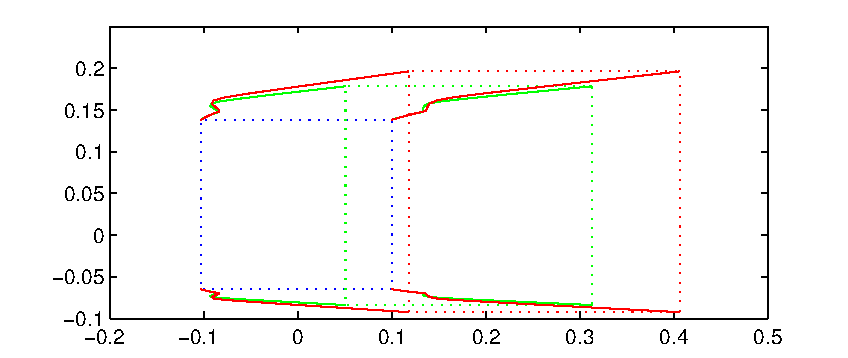
\includegraphics[scale=.8]{Chap4-Visual-Servoing/comparison_linearization}
 \caption{\label{Fig:Results5}\small{In this figure, we show the trajectory of the visual features in one iteration of the QP, and compare the evolution of the features obtained by the linearization model (green lines) and features obtained by the exact non-linear model (red lines).}}
 \end{figure}

Due to the walking nature, we have oscillations in the features trajectories. One of the main advantages of using MPC is that it naturally filters out these oscillations because we minimize the errors in a full cycle. It is remarkable that, in comparison with the decoupled approach ~\citep{DuneIROS2010} we do not need to model explicitly the sway motion of the robot and the resulting motion of the visual features. The system could oscillate inside the horizon (and it does), but at the end, the optimal control is taken without oscillations (Fig.~\ref{Fig:Results6}). In Fig.~\ref{Fig:Results6}, we only show three features errors evolution, the $u$ component of each left (black) and right (red) lower side corners, since the upper ones are, by symmetry, the same. And we complete with a single $v$ component (blue) for all the corners, with the same symmetry argument. 

\begin{figure}[ht]
 \centering
 %\subfigure[]{
 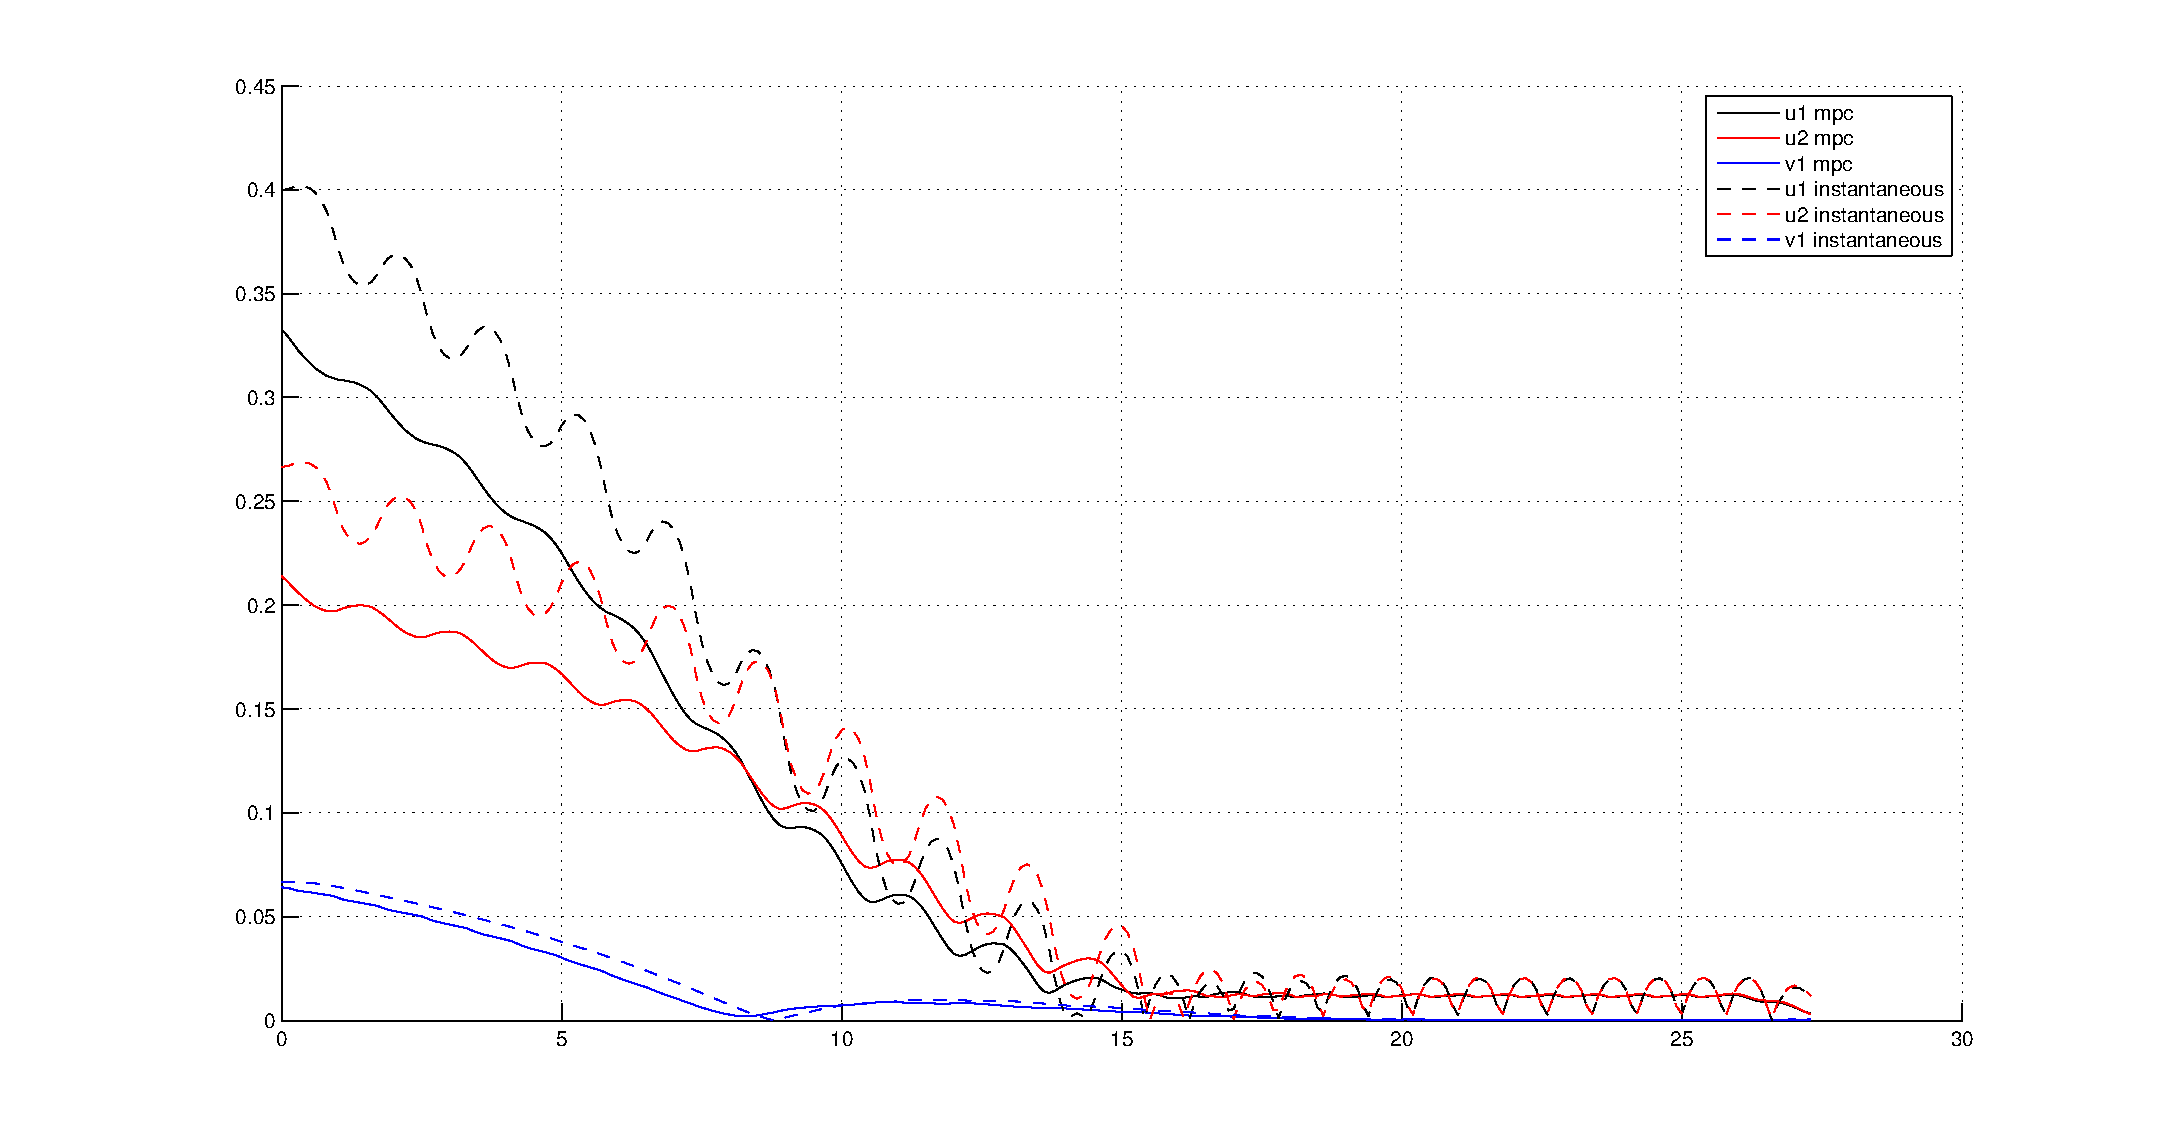
\includegraphics[scale=.35]{Chap4-Visual-Servoing/errors_mpc_instantaneous}
 \label{Fig:Results6a}
 %}
 % \subfigure[]{
 %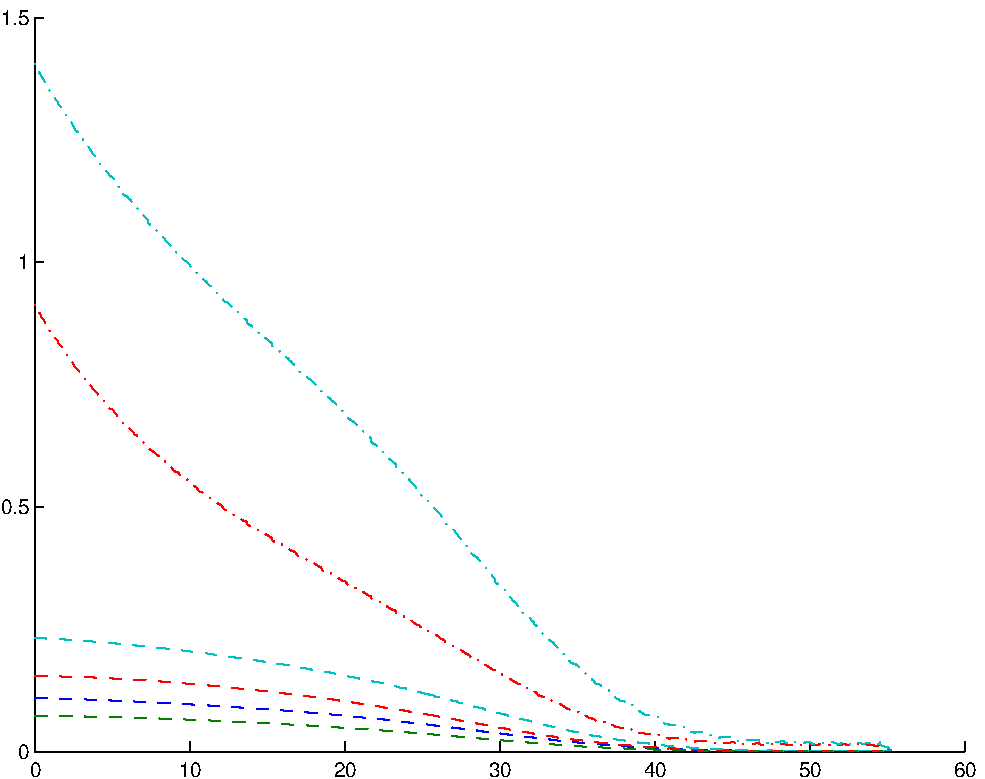
\includegraphics[scale=.23]{./figures/horizon_errors}
 %\label{Fig:Results6b}
 %}
 \caption[]{\label{Fig:Results6}\small{Evolution of the errors for the $u,v$ components of each feature, in the second simulation. In dashed line, we depict the instantaneous errors along time, and in solid line, we depict the errors estimated in the horizon (i.e. individual terms of Eq.~ \ref{Eq:MinVisualFeatures2}, normalized by the size of the horizon). Observe that the sway motion of the robot induces oscillations of the $u$ components in the instantaneous errors, and that these oscillations are not present in the errors estimated in the horizon window.}}
 \end{figure}

\subsection{Comparisons: coupled vs. decoupled approaches}

\begin{figure*}[ht]
 \centering
 \subfigure{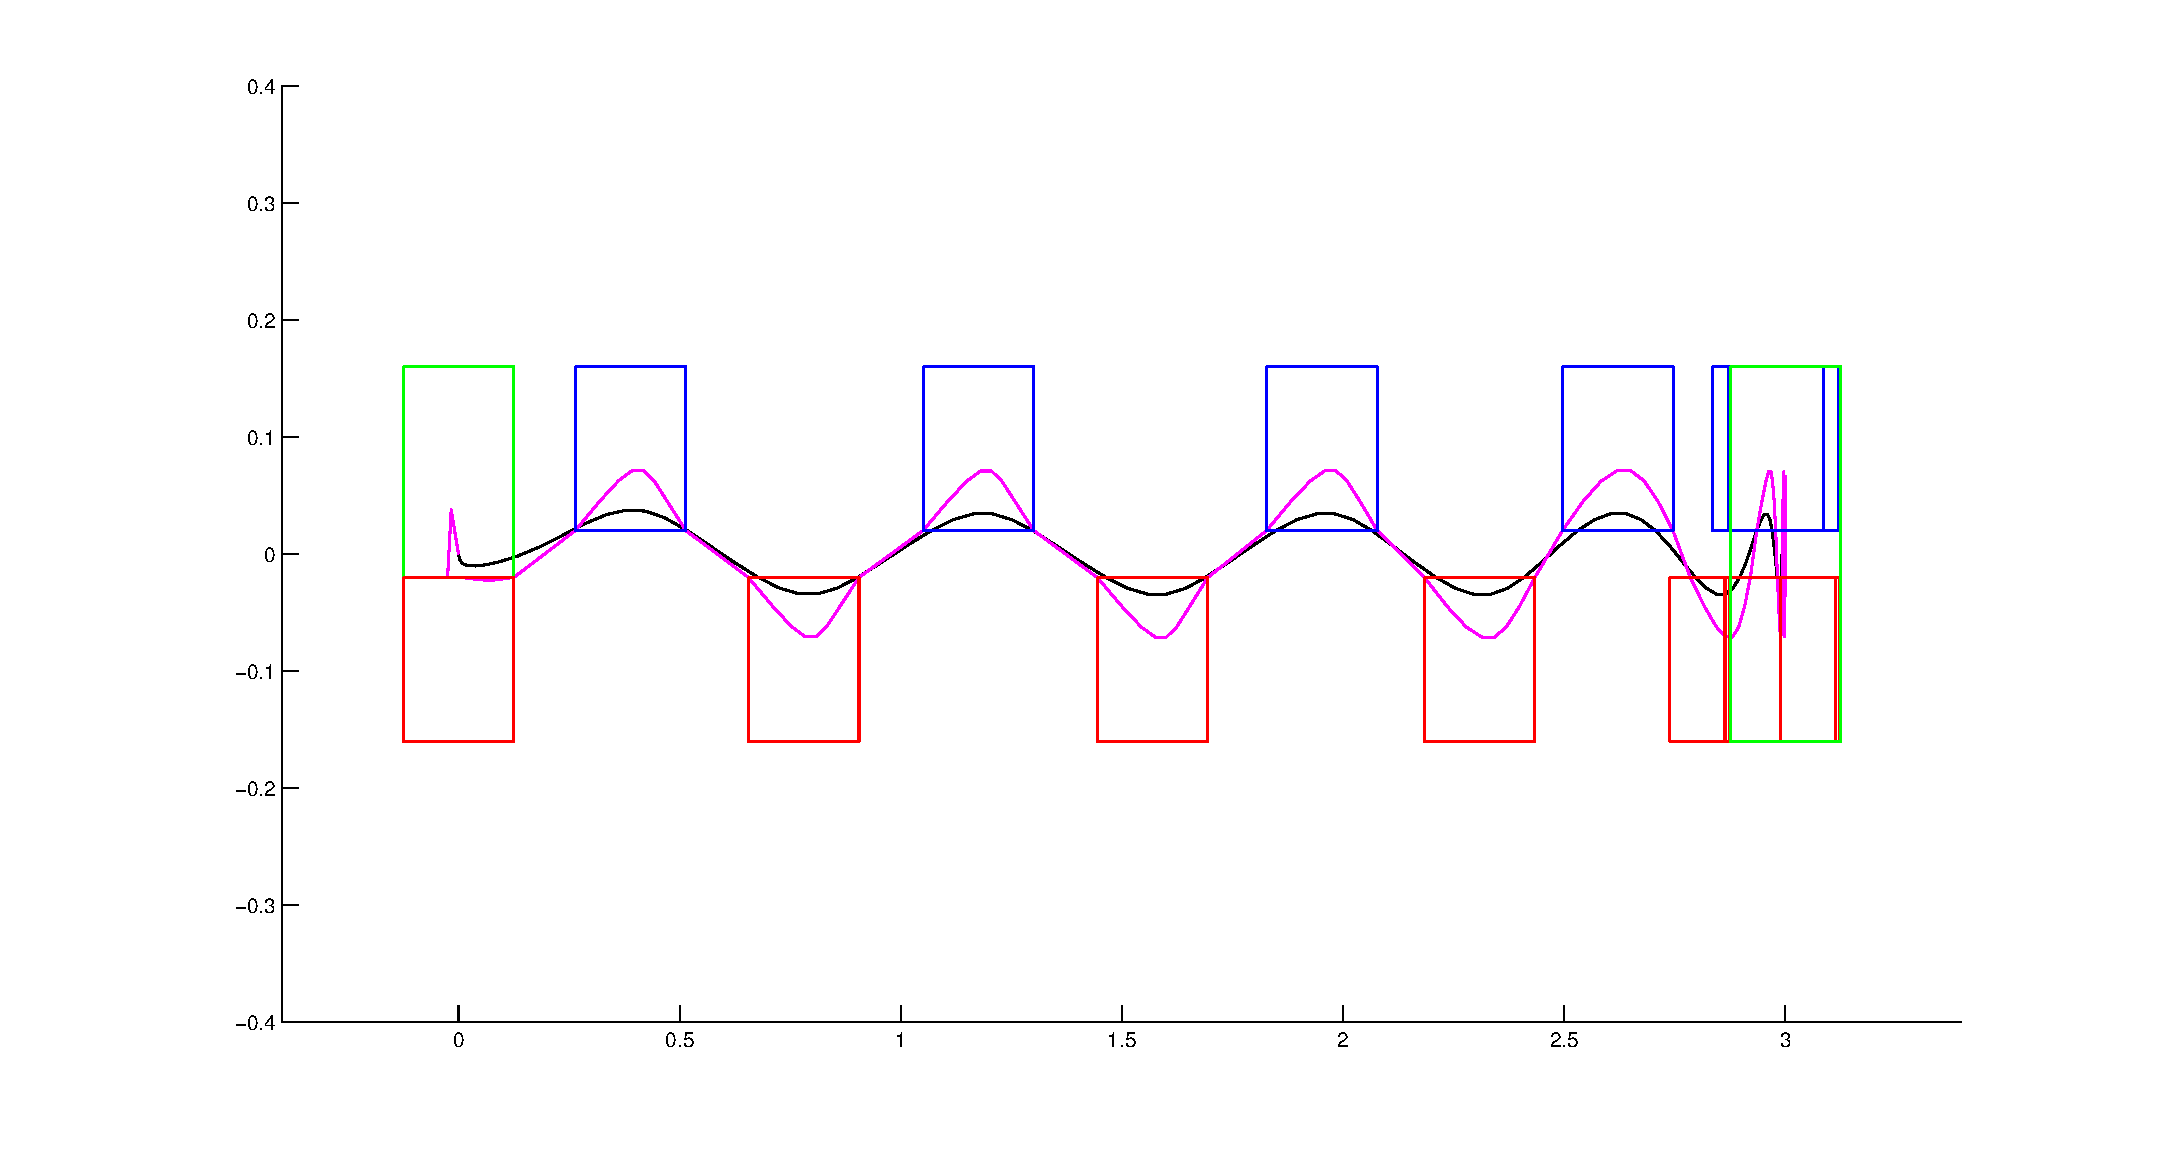
\includegraphics[scale=.18]{Chap4-Visual-Servoing/footsteps_mpc}} ~
 \subfigure{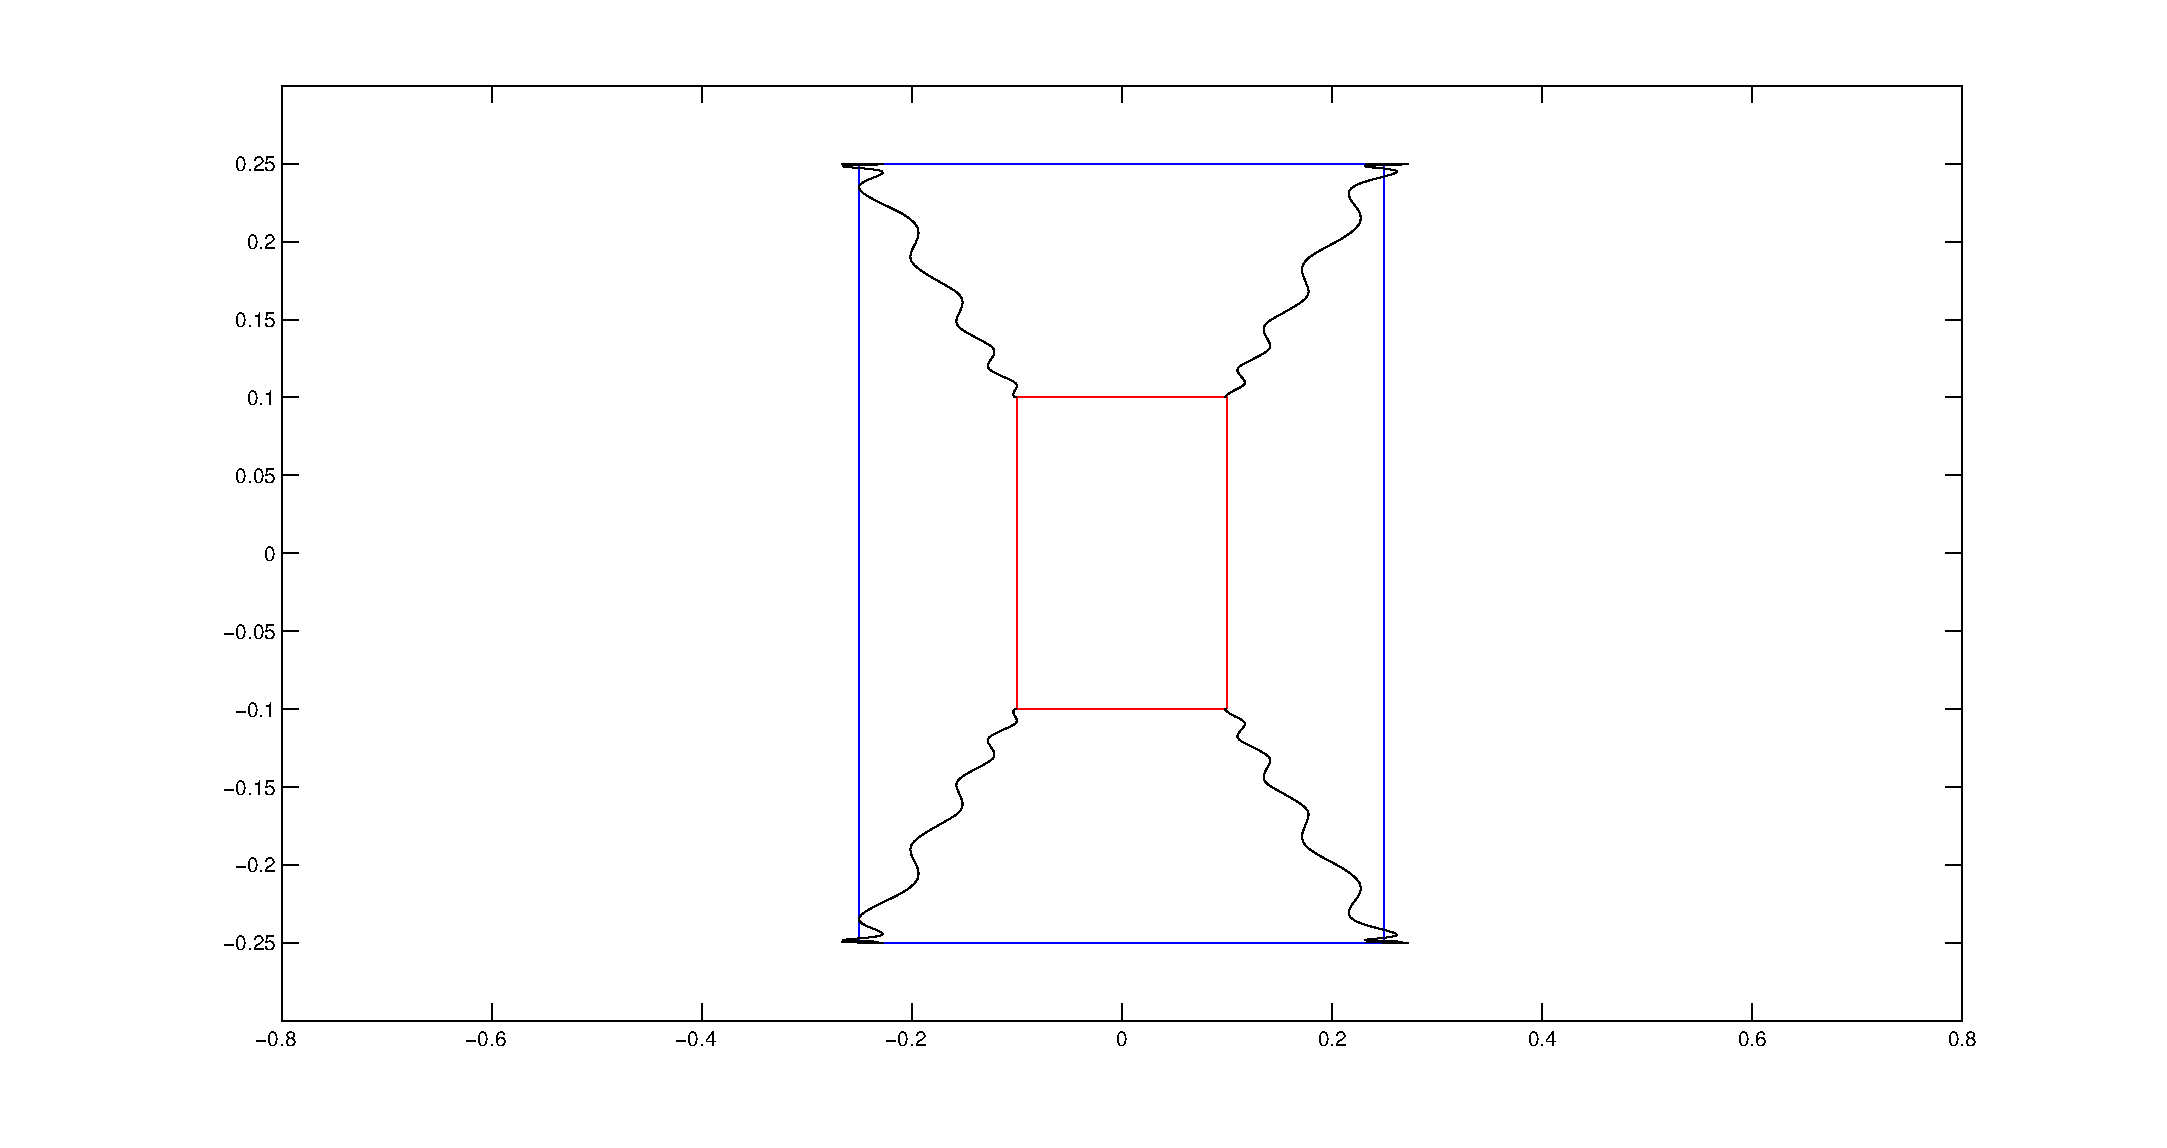
\includegraphics[scale=.18]{Chap4-Visual-Servoing/features_mpc}} \\
 \subfigure{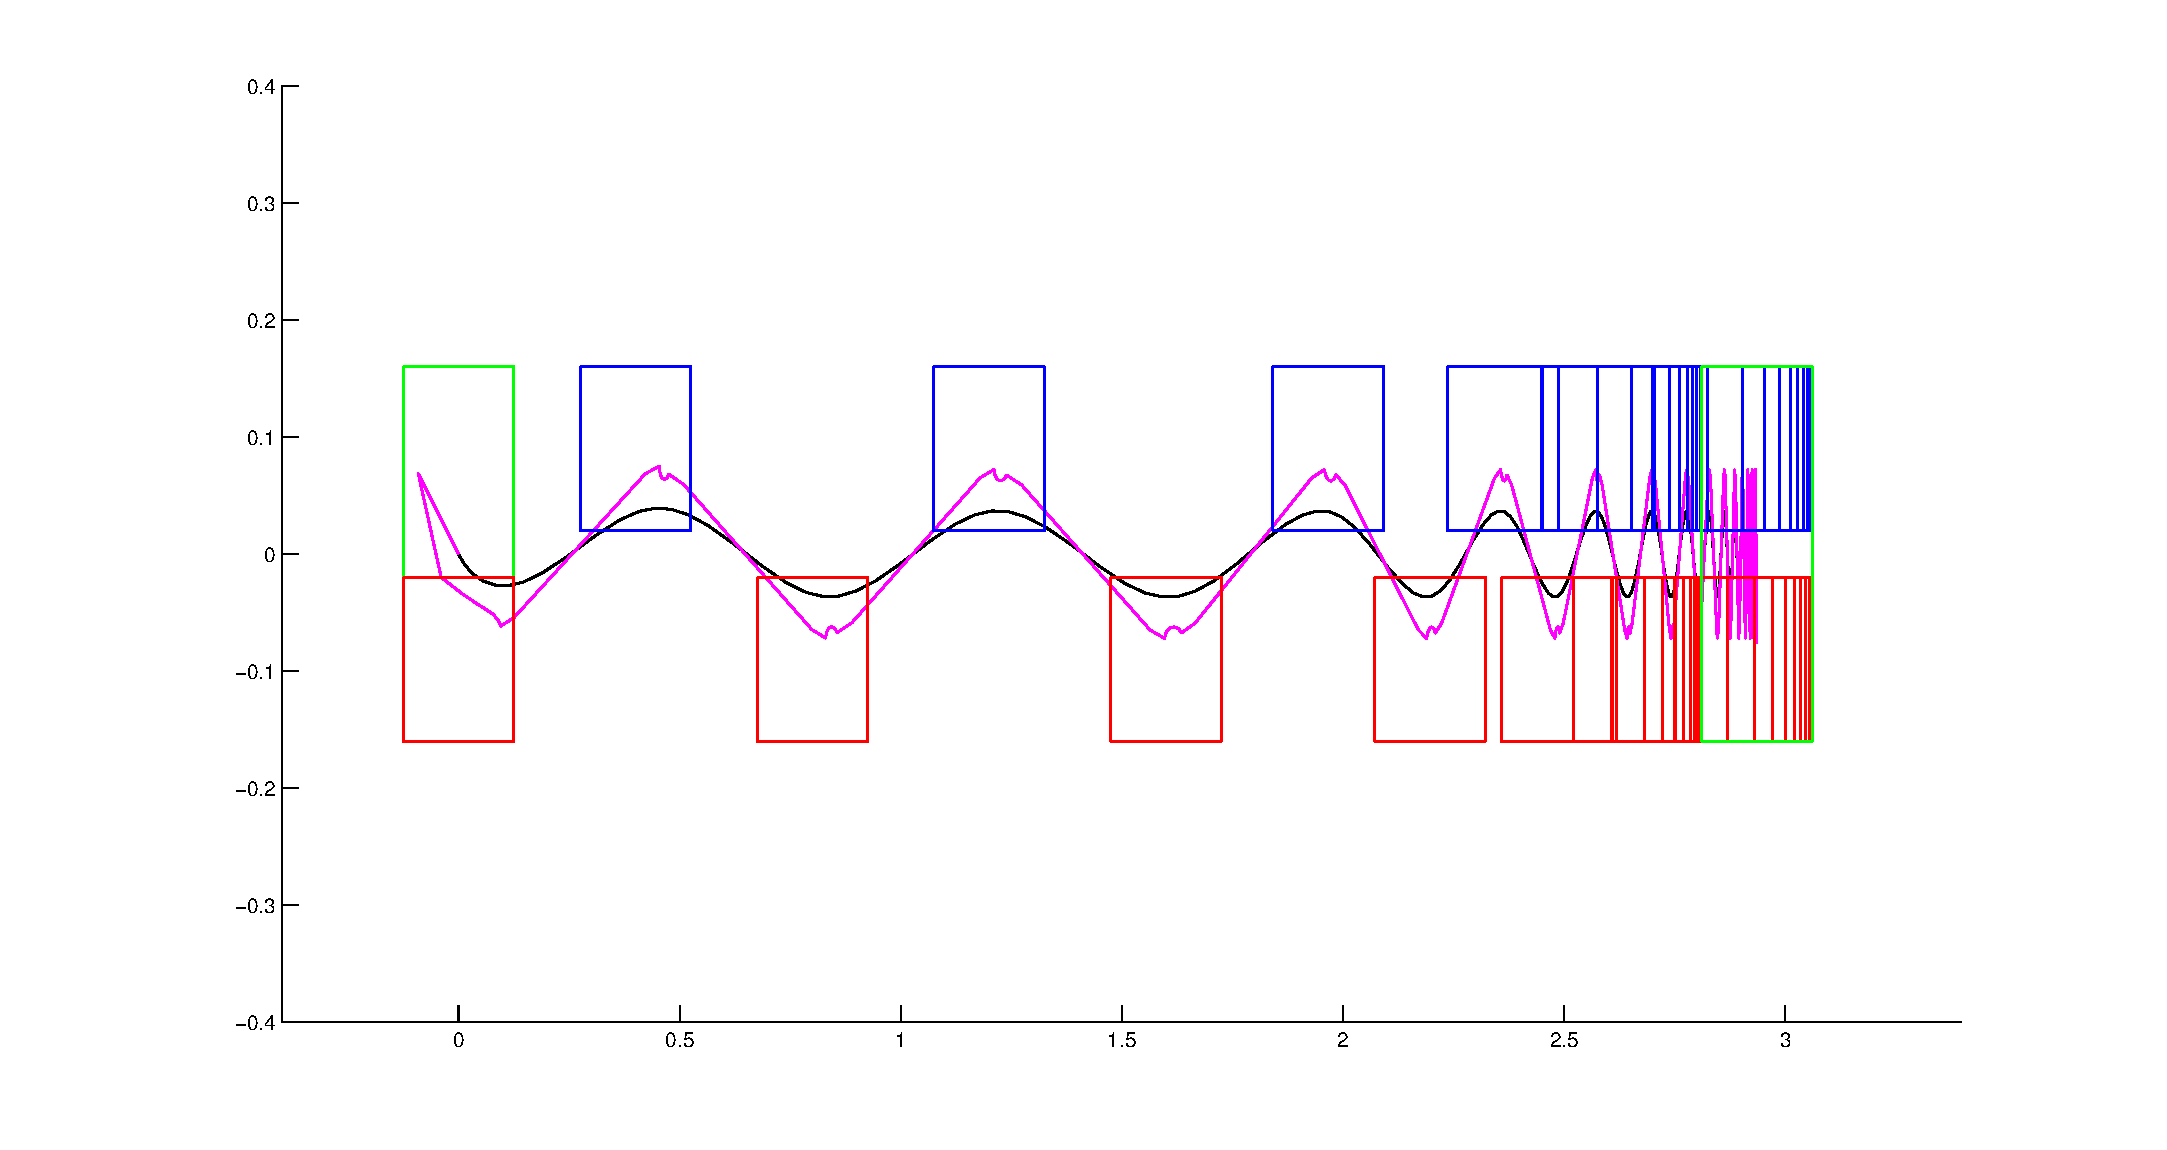
\includegraphics[scale=.18]{Chap4-Visual-Servoing/footsteps_classical-vs}} ~
 \subfigure{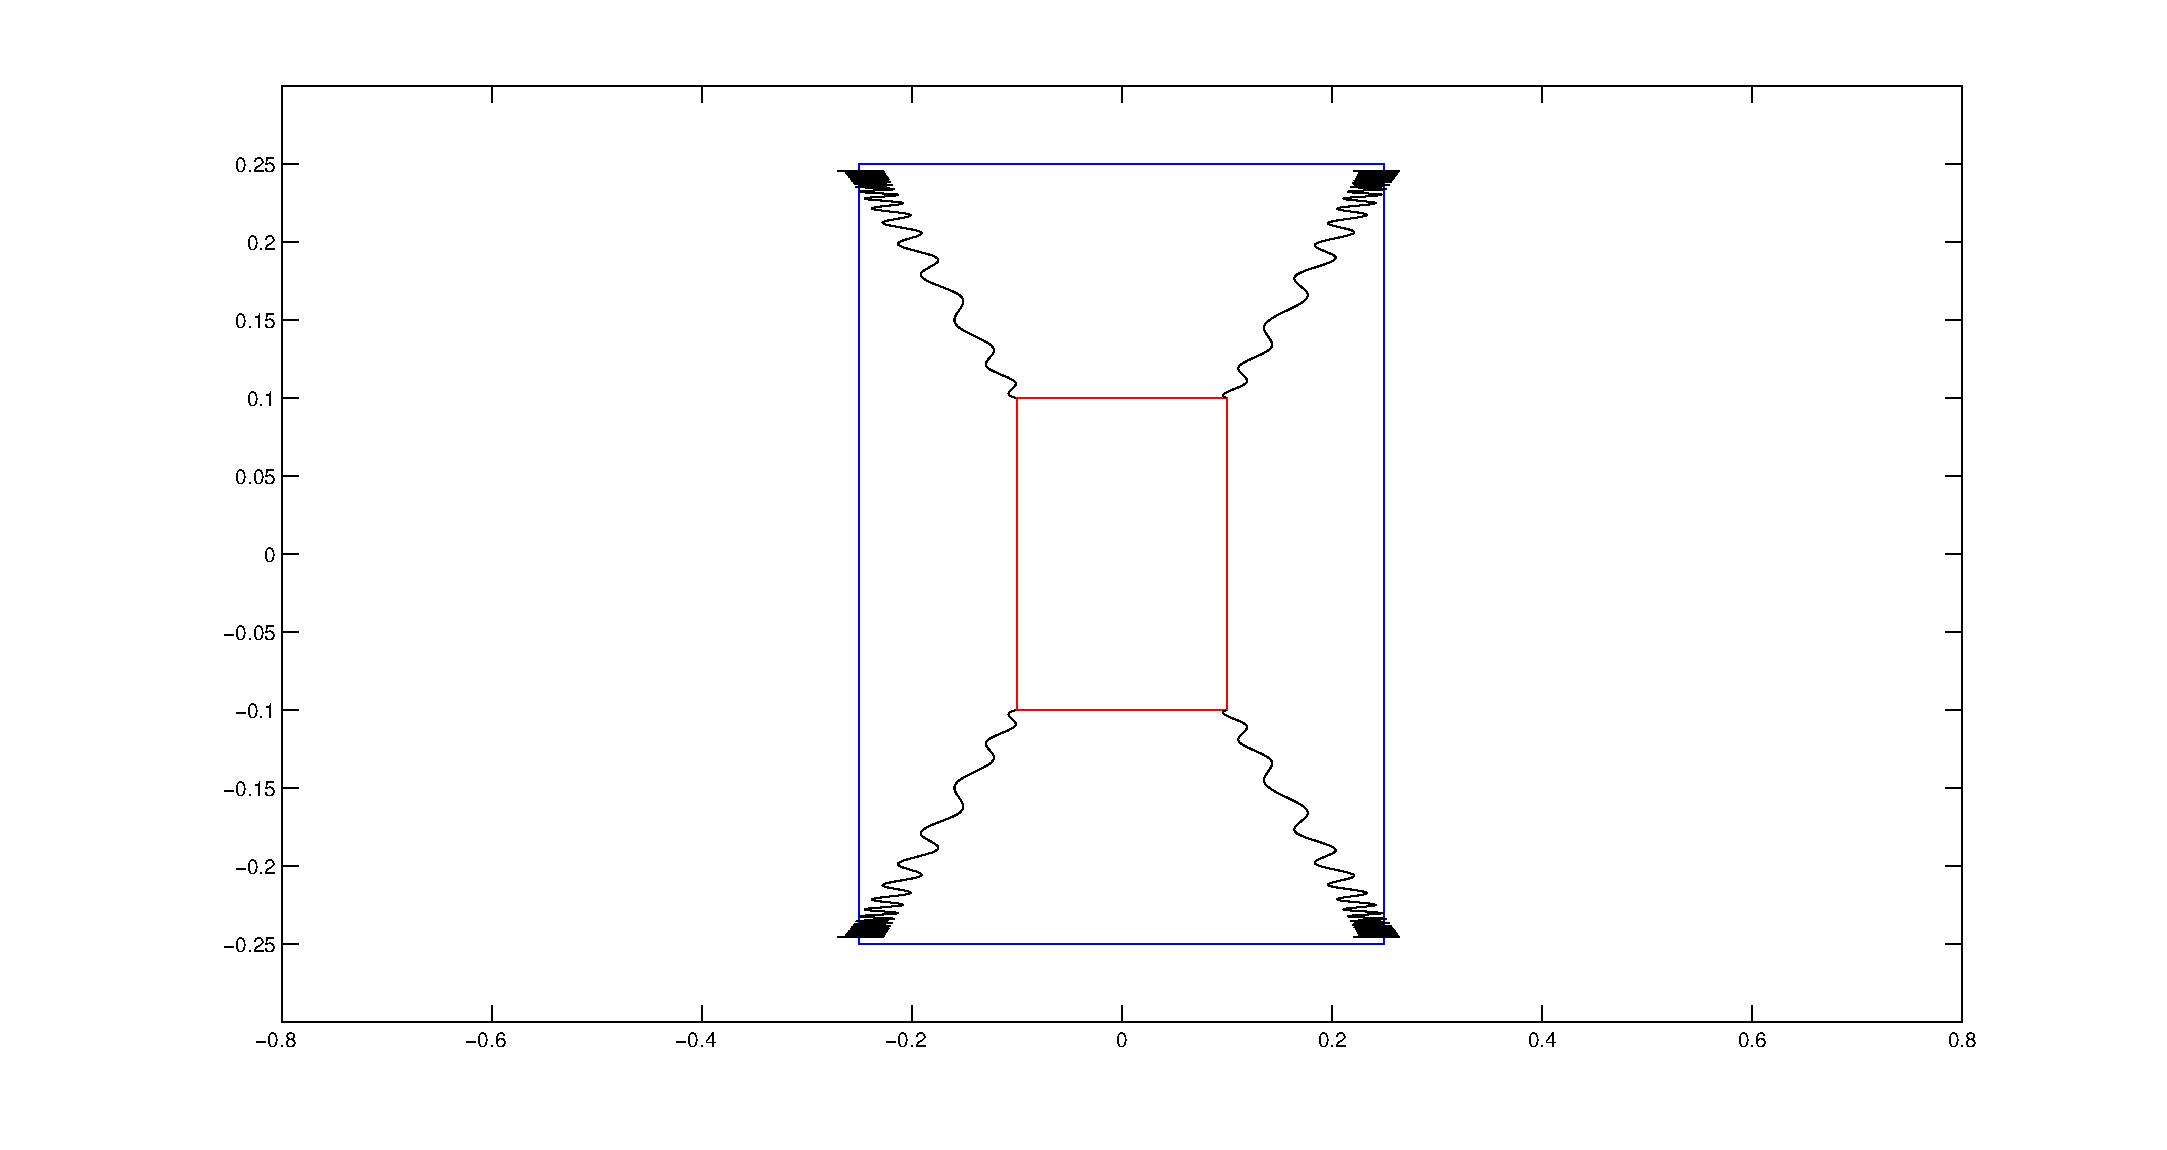
\includegraphics[scale=.18]{Chap4-Visual-Servoing/features_classical-vs}}
 \caption{\label{Fig:Comparisons-approaches} Comparison between the coupled (upper part) and decoupled approaches (lower part). On the left side, we depict the robot trajectory with the footsteps (red and blue), and the CoM (black) and CoP (pink) trajectories. On the right side, we depict the evolution of the instantaneous features positions during the experiment (from the red rectangle, at the beginning of the simulation, to the blue one, at the end).}
 \end{figure*}

\begin{figure*}[ht]
 \centering
 \subfigure{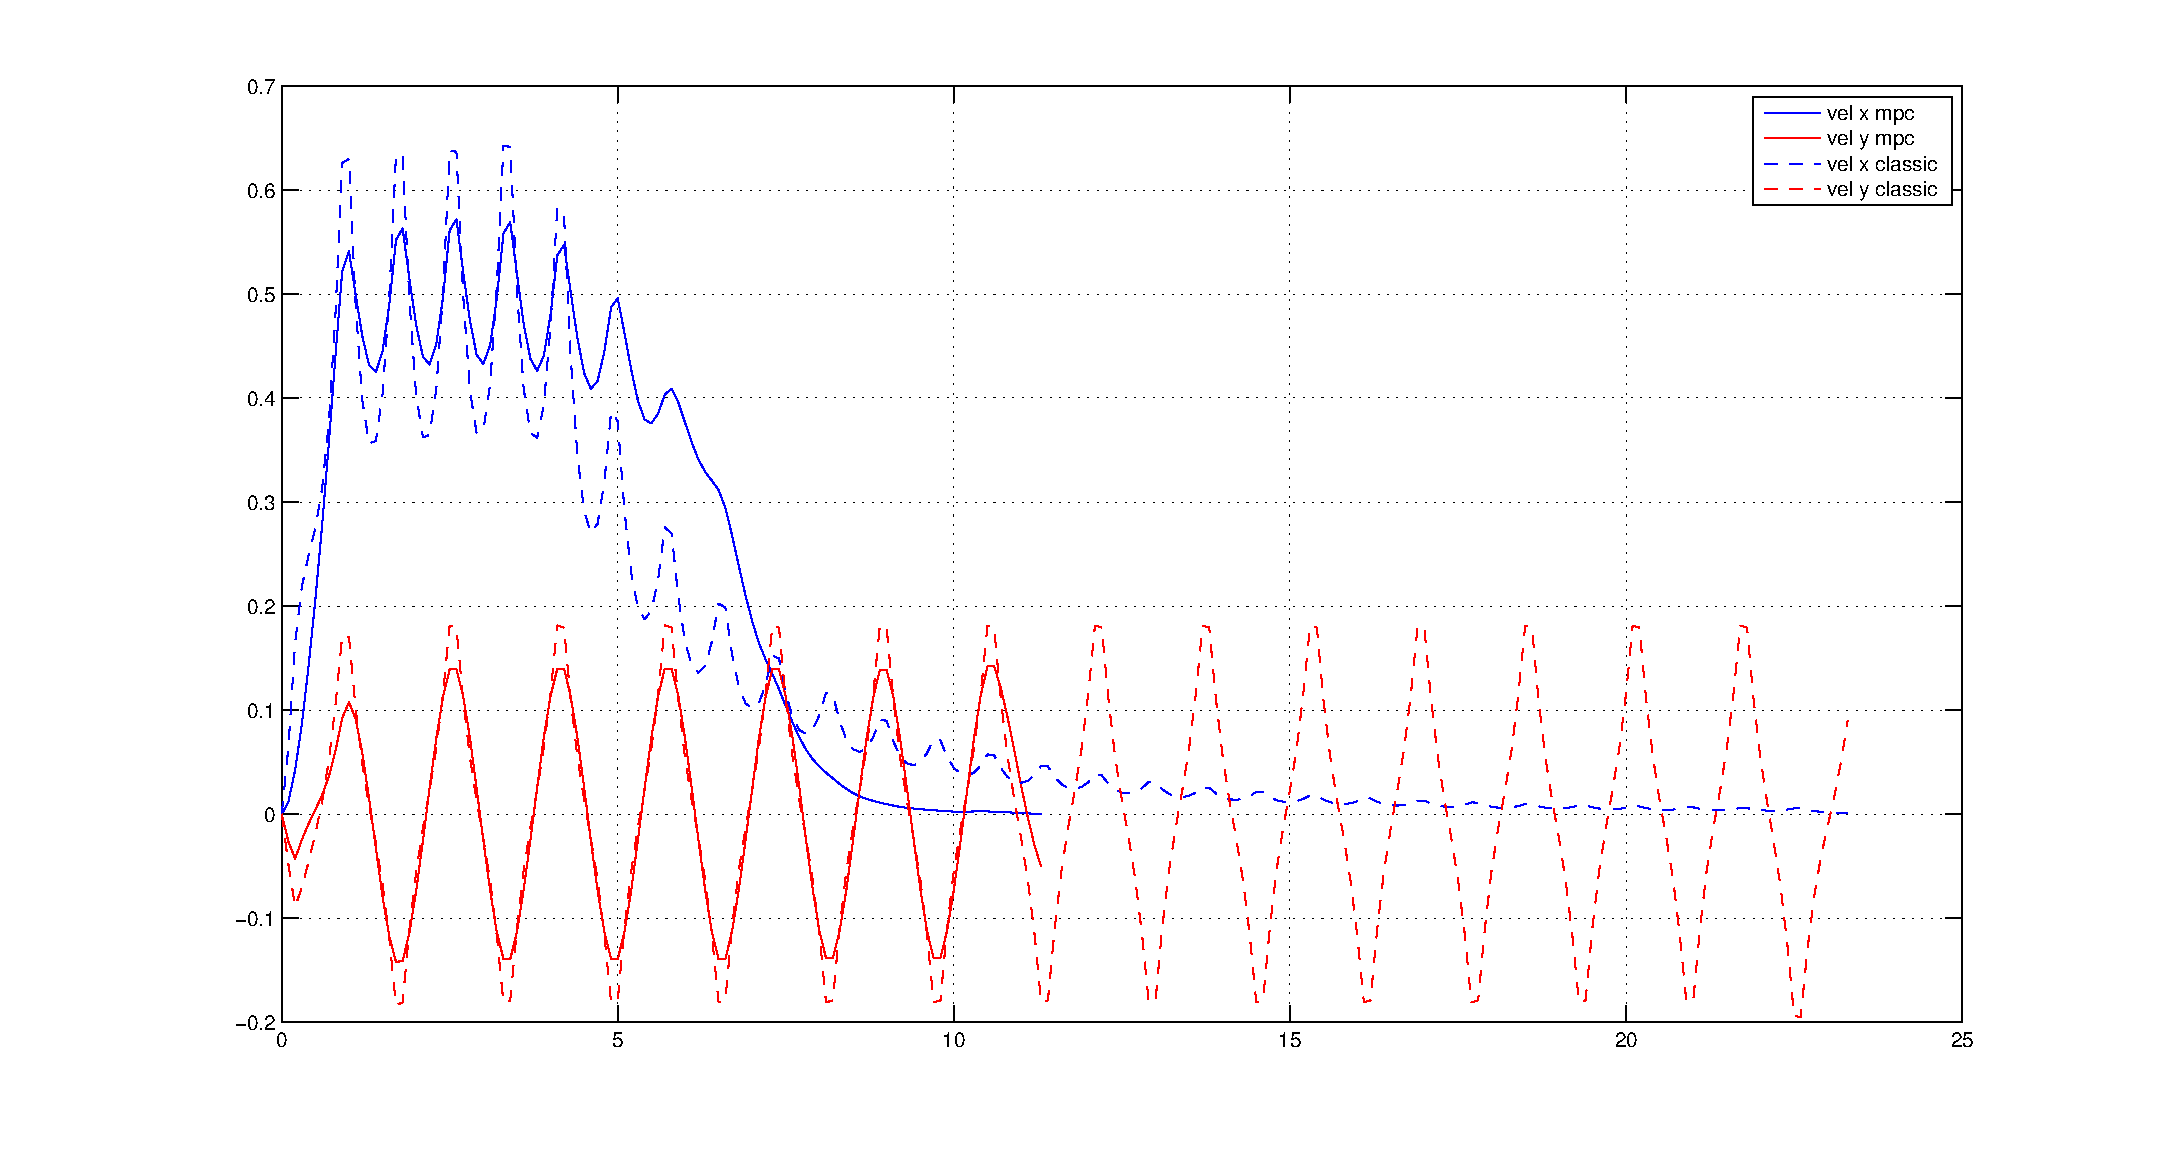
\includegraphics[scale=.3]{Chap4-Visual-Servoing/velocities_both}}
 \subfigure{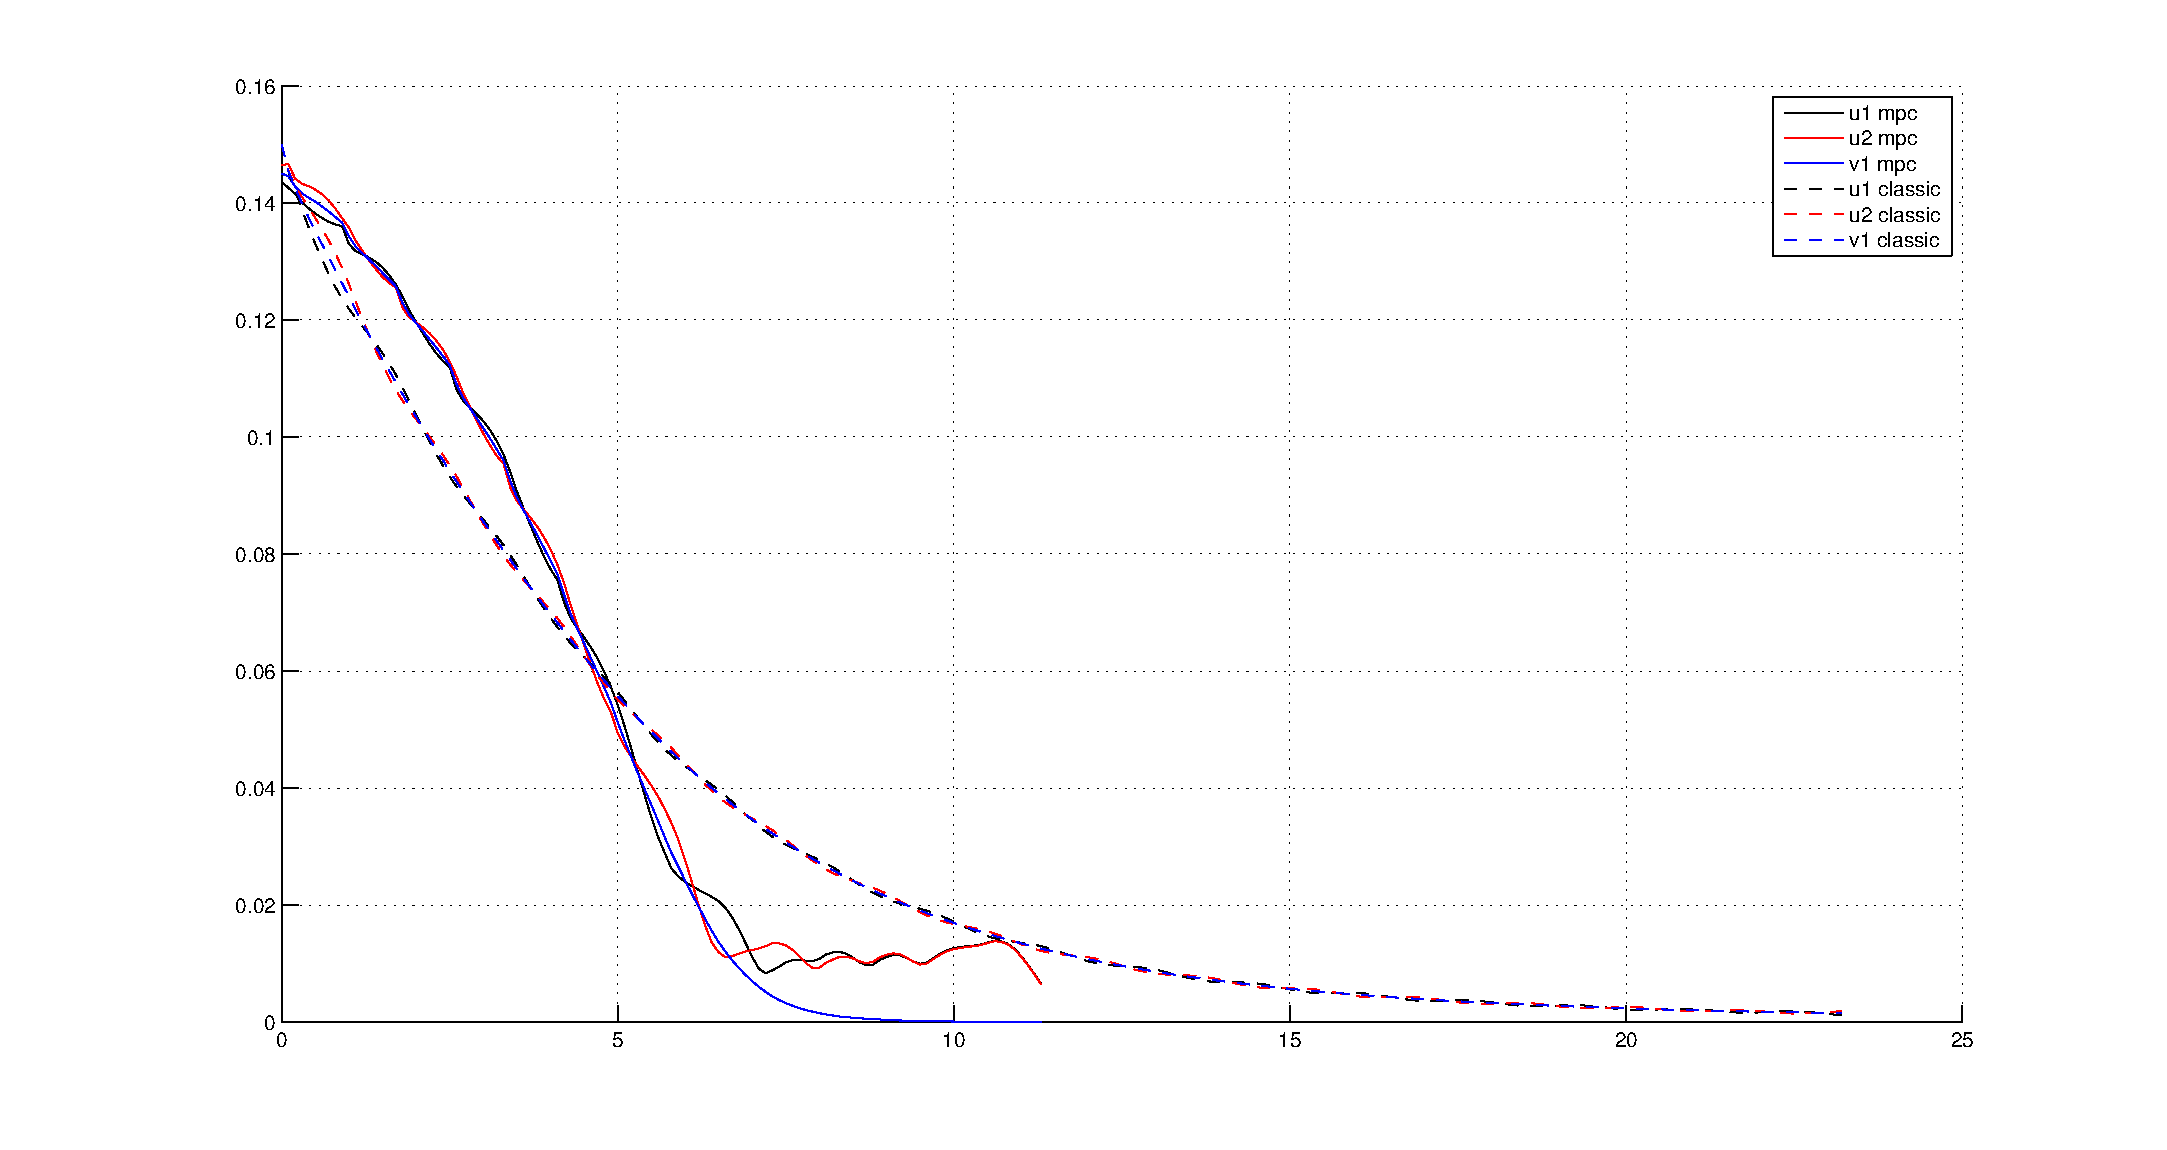
\includegraphics[scale=.3]{Chap4-Visual-Servoing/errors_both}}
 \caption{\label{Fig:Comparisons-velocitieserrors} Left, comparison of velocity profiles in the $x$ (blue) and $y$ (red) axis, for the decoupled (dashed line) and coupled (solid line) approaches. Right, comparison of the features errors evolution.}
 \end{figure*}

We conducted a simple experiment to illustrate better the differences between the two approaches of Section~\ref{sec:vsclaire} and Section~\ref{sec:vsmauricio}, and to have quantitative comparisons between them. In this experiment, the robot has simply to go three meters forward. In Fig.~\ref{Fig:Comparisons-approaches}, we depict the robot trajectories and footsteps (left column) and the features trajectories (right column) for each approach (the coupled one in the upper line, the decoupled one in the lower line). We can clearly appreciate that the coupled approach converges faster. Indeed, with the coupled approach, it took 15 steps (including double supports) to reach the goal. However, with the decoupled approach, after 30 steps, the goal  has still not been reached and keeps converging slowly. Here, the convergence criterion is the norm of the errors between the current features positions and the desired ones. Moreover, one can observe that, close to the goal, the features positions follow a smoother trajectory in the case of the visual predictive control than with the decoupled approach, where oscillations (as a result of the immediate stepping) are visible.

In Fig.~\ref{Fig:Comparisons-velocitieserrors} left, we present the profiles of velocities performed by the robot, in both cases. It is interesting to note that in the coupled approach, the amplitude of the oscillations is smaller, which is desirable. Also, when the error gets small, the classical approach slows down to have a slow convergence rate. This is a normal feature of classical visual servoing, i.e. the error evolves with an exponential decay. In the decoupled approach, this behavior is clearly present. However, in the coupled approach combining the MPC walking pattern generator with visual predictive control, this is not true anymore, see Fig.~\ref{Fig:Comparisons-velocitieserrors} right, in particular, because we take into account future information, so the coupled system converge faster. In the errors evolution, we use the same symmetry argument as in Fig.~\ref{Fig:Results6}. We should note that the $u$ components in the image plane are theoretically the oscillatory ones (from the stepping motion). In Fig.~\ref{Fig:Comparisons-velocitieserrors}, we can see that the $v$ component converges faster in the coupled approach. With the $u$ components, there remains a small residual of the oscillation in both the coupled and decoupled approaches, which explains that the $u$ components converge slower in the coupled approach.


\section{Conclusion}
\label{sec:conclusions}
Since the original proposal for walking generation proposed in~\citep{Kajita2003}, most of the efforts in the literature have focused in dynamical balance and stability. In this chapter, we have proposed a novel approach to close the control loop by introducing visual information into the walking pattern generation. Our online pattern generator integrates the regulation of the relative pose of 3D image features while simultaneous ensuring safety and stability. In order to keep the optimization formulation as a QP, the perspective projection equations have been linearized around the features positions at the beginning of each cycle. However, our current approach uses 3-D information that strongly depends on the localization. As an ongoing work, we wish to drop the need of 3-D information by predicting the image positions of the landmarks in terms on the velocity of the robot in the horizon (IBVS); we also plan to perform real experiments on the HRP-2 humanoid platform.


% Using planning
\chapter{Planning Visual Tasks for Reactive Humanoid Walking} 
\label{Chap:Visual-Planning}

In the previous chapter, we presented a scheme to control a humanoid robot directly by using visual servoing techniques. However, the trajectories realized by the robot in that case are generated to minimize the distance in the image features space and might create unnecessary motion in the space of the footprints. This is because visual servoing is a local control technique. If we want to take into account the shape of the trajectory or obstacles avoidance, a planning method would be necessary.

Motion planning aims to take the robot from an initial to a final position while ensuring feasibility and obstacle avoidance. The notion of optimality arises in motion planning. From the work of \citep{Salaris:2010, jib-IJHR2010}, it exists a set of optimal trajectories to take a nonholonomic robot, evolving in free space, from an initial to a final position while keeping in sight a landmark. Also, it has been shown that the human walking behaves nonholonomic for open spaces. In this chapter, we will work upon those works and we will inject the motion primitives from the planner into the pattern generator level of the robot.

\section{Global planning with visibility constraints}
%==================================================================

\label{sec:globalplanning}

For visual servoing, localization, surveillance, or any robotic task based on the observation of visual cues, it is important to ensure that the robot under control does not lose sight of the landmark(s) used as a visual reference. Hence, several works have been proposed to provide motion planners that guarantee landmark visibility, mainly for wheeled robots.

With this concern in mind, we borrow one such global planner, described in~\citep{jib-IJHR2010},  as a base tool for generating paths that guarantee to enforce the required visual constraints while giving locally optimal trajectories in distance. This base planner for humanoid robots uses as an underlying model of motion, a disk-shaped non-holonomic Differential Drive Robot (DDR). In~\citep{jib-IJHR2010}, if a solution path is found for the DDR, it is converted into a solution path for the humanoid robot by generating a footprints sequence coherent with the humanoid dimensions. A nice property inherited from using the DDR model of motion is that the global planner is complete, i.e.  if a solution exists, it will give one, otherwise, it will say so.

However, even if, locally, the used motion primitives are optimal in distance, this approach does not necessarily give globally optimal trajectories. We will not detail the complete methodology here, but we recall the basic results hereafter.

The aforementioned algorithm takes as an input a 2D map of the environment, with its obstacles and visual landmarks, an initial configuration of the robot in the plane, $(x_A,y_A,\theta_A)$, and a final (goal) configuration in the plane, $(x_B,y_B,\theta_B)$. Its output is a set of footprints in the plane to be followed by the robot. The building of this path follows a classical recursive strategy: A roadmap is built over the free space, which includes both, points free of collision with the obstacles in the environment and points that are not within the shadows cast by the landmarks. Then, the initial and final configurations are tested, to check whether the optimal primitives of~\citep{Salaris:2010} can connect them without colliding with forbidden regions. If the computed path is without collision, then the algorithm ends, otherwise the holonomic shortest path on the roadmap from the initial configuration to the final (if it exists) is divided in two parts by its middle point, and the whole process is repeated on the two sub-parts. 

The resulting path is made of several parts, each one corresponding to a locally optimal path given from~\citep{Salaris:2010} (made of a combination of straight lines, logarithmic spirals and in-site rotations). This allows to define a set of $S$ sub-segments to be performed by the robot along locally optimal paths, which will be referred to as $(p^s,q^s)$, for $s=1\dots S$~:
$$
p^s = (x_p^s,y_p^s,\theta_p^s)^T \; ; \; q^s = (x_q^s,y_q^s,\theta_q^s)^T,
$$

with $p^s$ the initial configuration and $q^s$ the final one. The complete computed path is executed by reaching the successive sub-goals $q^s$.


%==================================================================
\section{Defining a local reference trajectory}
%==================================================================

\label{sec:reftrajectories}

Let us focus on the execution of each sub-path $s$. Suppose that we start with the robot at some configuration close to $p^s$ (see Fig.~\ref{fig:paths}), because localization may not be perfect, and suppose that we want to reach the final configuration or sub-goal $q^s$, as determined in~\citep{jib-IJHR2010}.

\subsection{Adapting the reference trajectory for the MPC}

Without loss of generality, we suppose that the object of interest to be kept at sight by the robot is located at $L^s = (0,0)$. In all the following, $x,y,\theta$ will refer to coordinates w.r.t a global frame centered at this origin.

It is noteworthy that, given the sub-goal $q^s =(x_q^s,y_q^s,\theta_q^s)^T$ to reach, and the landmark it is associated to, the work of~\citep{Salaris:2010} gives us a full synthesis of optimal paths in free space. This synthesis can be represented as a mapping $\sigma$:
$$
\begin{array}{cccccc}
\sigma & : & \mathbb{R}^2 & \mapsto & \mathbb{S}^1 \times \mathbb{R}^2\\
& & (x,y) & \rightarrow & (\theta^*(x,y),v^*(x,y),\omega^*(x,y))
\end{array}
$$

where $\theta^*(x,y)$ is the orientation the robot (viewed as a nonholonomic cart)  should have in order to start walking along the shortest path to $q^s$, from its current position $(x,y)$. The pair $(v^*(x,y),\omega^*(x,y))$ are the instantaneous (reference) velocities needed to be applied to follow the shortest paths. Without loss of generality, we can suppose that $v^*(x,y)=0$ (for in-site rotations) or $v^*(x,y)=\pm 1$ (elsewhere). Given the linear velocity $v^*(x,y)$, $\omega^*(x,y)$ is defined in function of the nature  of the path segment,
$$
\left\{
\begin{array}{cccc}
 \omega^*(x,y) & = & 0 & \mbox{(straight line)}\\
  & = & \pm\frac{\sin(\phi_{max})}{\sqrt{x^2+y^2}} & \mbox{(spiral)},\\
\end{array}
\right.
$$

where $\phi_{max}$ is the maximal bearing angle possible for the landmark, given the sensor and robot characteristics.

Our claim is that the knowledge of optimal policies at each point allows some flexibility when generating a walking pattern, by optimizing the footprint positions and  the CoM trajectory ``around'' the nominal path output from the planner, by using these policies within the pattern generation.

\begin{figure}[h]
\centering
 \scalebox{1.5}{\subimport*{Chap5-Visual-Planning/}
                   {config.pdf_t}}\hspace{2cm}
\caption{From a configuration $(x,y,\theta)$ and its corresponding position $(x,y)$, and a sub-goal $q^s= (x_q^s,y_q^s,\theta_q^s)$ to reach, the optimal path (dashed line) is the one we want the humanoid robot to follow. For that, we use the tangent orientation $\theta^*(x,y)$ to this path. Because of the errors in control or localization, this optimal path may be different from the shortest path (solid line) computed from the first configuration $p^s= (x_p^s,y_p^s,\theta_p^s)$.
%For the linearization purposes, and given that $(x,y)$ will be variable, we will use a nominal shortest path (solid line) from a close, fixed configuration $p^s= (x_p^s,y_p^s,\theta_p^s)$.
\label{fig:paths}}
\end{figure}

In pattern generation algorithms such as~\citep{HerdtAR2010}, the cost function within the Model Predictive Control (MPC) window uses the configurations of the CoM (see Chap.~\ref{Chap:Locomotion-Control}). Here, focusing more specifically on the $(x,y,\theta)$ CoM coordinates, we handle as an input of the algorithm a reference trajectory to be followed, and a synthesis of shortest paths leading to a given objective, as a direct output from~\citep{Salaris:2010}. As depicted in Fig.~\ref{fig:paths}, at each configuration evaluated within the MPC, two forces should apply through the optimization scheme: one driving the robot to the ``correct'' orientation $\theta^*(x,y)$, and one making the velocities follow the shortest path, $(v(x,y),\omega(x,y))$, so we can follow the trajectories according to the optimal synthesis. Also, a strong visibility constraint should apply, to ensure the object of interest to stay visible. In Fig.~\ref{fig:fieldNoLateral}, we give an illustration of the shortest paths synthesis from~\citep{Salaris:2010}, displayed through the local orientations of optimal paths at each point of the plane, given the objective to reach (``end point'') and the landmark to keep in sight. 


%==================================================================
%\subsection{Tracking a single reference trajectory}
%==================================================================

%\label{subsection-singleref}

%In that case, we would track the reference path from $p^s$ to $q^s$; this has the advantage of being rather simple to express, I believe. Consider the reference path from $p^s$ to $q^s$; generate a corresponding sampled trajectory  $x_{ref}(k\tau),y_{ref}(k\tau),\theta_{ref}(k\tau)$, then stack them into vectors $C^x_{ref},C^y_{ref},C^\theta_{ref}$. Note that from the same analysis, we could also reinforce the tracking of the desired trajectories by including reference velocities, 

%$$
%\left\{
%\begin{array}{ccc}
%\dot{x}_{ref}(k\tau) & = & v \cos(\theta_{ref}(k\tau)) \\
%\dot{y}_{ref}(k\tau) & = & v \sin(\theta_{ref}(k\tau)) \\
%\dot{\theta}_{ref}(k\tau) & = & \omega(v,x_{ref}(k\tau),y_{ref}(k\tau)) \\
%\end{array}
%\right.
%$$

%where $v$ is a reference linear velocity, and $\omega(v,x_{ref}(k\tau),y_{ref}(k\tau))$ directly deduced from the synthesis. Similarly to positions, these references velocities could be stacked into $\dot{C}^x_{ref},\dot{C}^y_{ref},\dot{C}^\theta_{ref}$.

%We would introduce directly this desired trajectory in the pattern generator, while keeping the decoupled formulation of~\cite{HerdtIROS2010}, for the $x,y$ position on the one hand, and for the $\theta$ angle, on the other. Hence,

%{\small
%\begin{eqnarray}
%\nonumber
% \min && \dfrac{\alpha}{2} \left\| C^x_{i+1} - C^x_{ref} \right\|^2 + \dfrac{\alpha}{2} \left\| C^y_{i+1} - C^y_{ref} \right\|^2 \\
%\nonumber
%&& + \dfrac{\beta}{2} \left\| \dot{C}^x_{i+1} - \dot{C}^x_{ref} \right\|^2 + \dfrac{\beta}{2} \left\| \dot{C}^y_{i+1} - \dot{C}^y_{ref} \right\|^2 \\
%\nonumber
%&& + \dfrac{\gamma}{2} \left\| F^x_{i+1} - Z^x_{i+1} \right\|^2 + \dfrac{\gamma}{2} \left\| F^y_{i+1} - Z^y_{i+1} \right\|^2 \\
%&& + \dfrac{\epsilon}{2} \left\| \dddot{C}^x_{i} \right\|^2 + \dfrac{\epsilon}{2} \left\| \dddot{C}^y_{i} \right\|^2,
%\end{eqnarray}
%}

%and for the angular position,

%{\small
%\begin{eqnarray}
%\nonumber
% \min && \dfrac{\alpha}{2} \left\| C^{\theta}_{i+1} - C^{\theta}_{ref} \right\|^2 + \dfrac{\beta}{2} \left\| \dot{C}^{\theta}_{i+1} - \dot{C}^{\theta}_{ref} \right\|^2 \\
%&& \dfrac{\gamma}{2} \left\| \sum (f^{\theta}_i - c^{\theta}_i) \right\|^2 
%\label{eq-opt-orientations}
%\end{eqnarray}
%}

%where $C^{\alpha}_{ref}$ with $\alpha \in \{x,y,\theta\}$ is the reference trajectory in the horizon, extracted from the trajectory generated with the planner \cite{HayetIJHR2010}.

%Note that the same process can be applied by considering, instead of $p^s$, the point corresponding to the current robot position. This would be a first, cheap way to adapt the reference trajectory. In both cases, the orientations would have been computed beforehand by Eq.~\ref{eq-opt-orientations}.

\begin{figure*}[h!]
\centering
%\vspace{2 mm}
%\hspace{5 mm}
 \subfigure[Motion direction field resulting from the synthesis of~\citep{Salaris:2010}.]{
  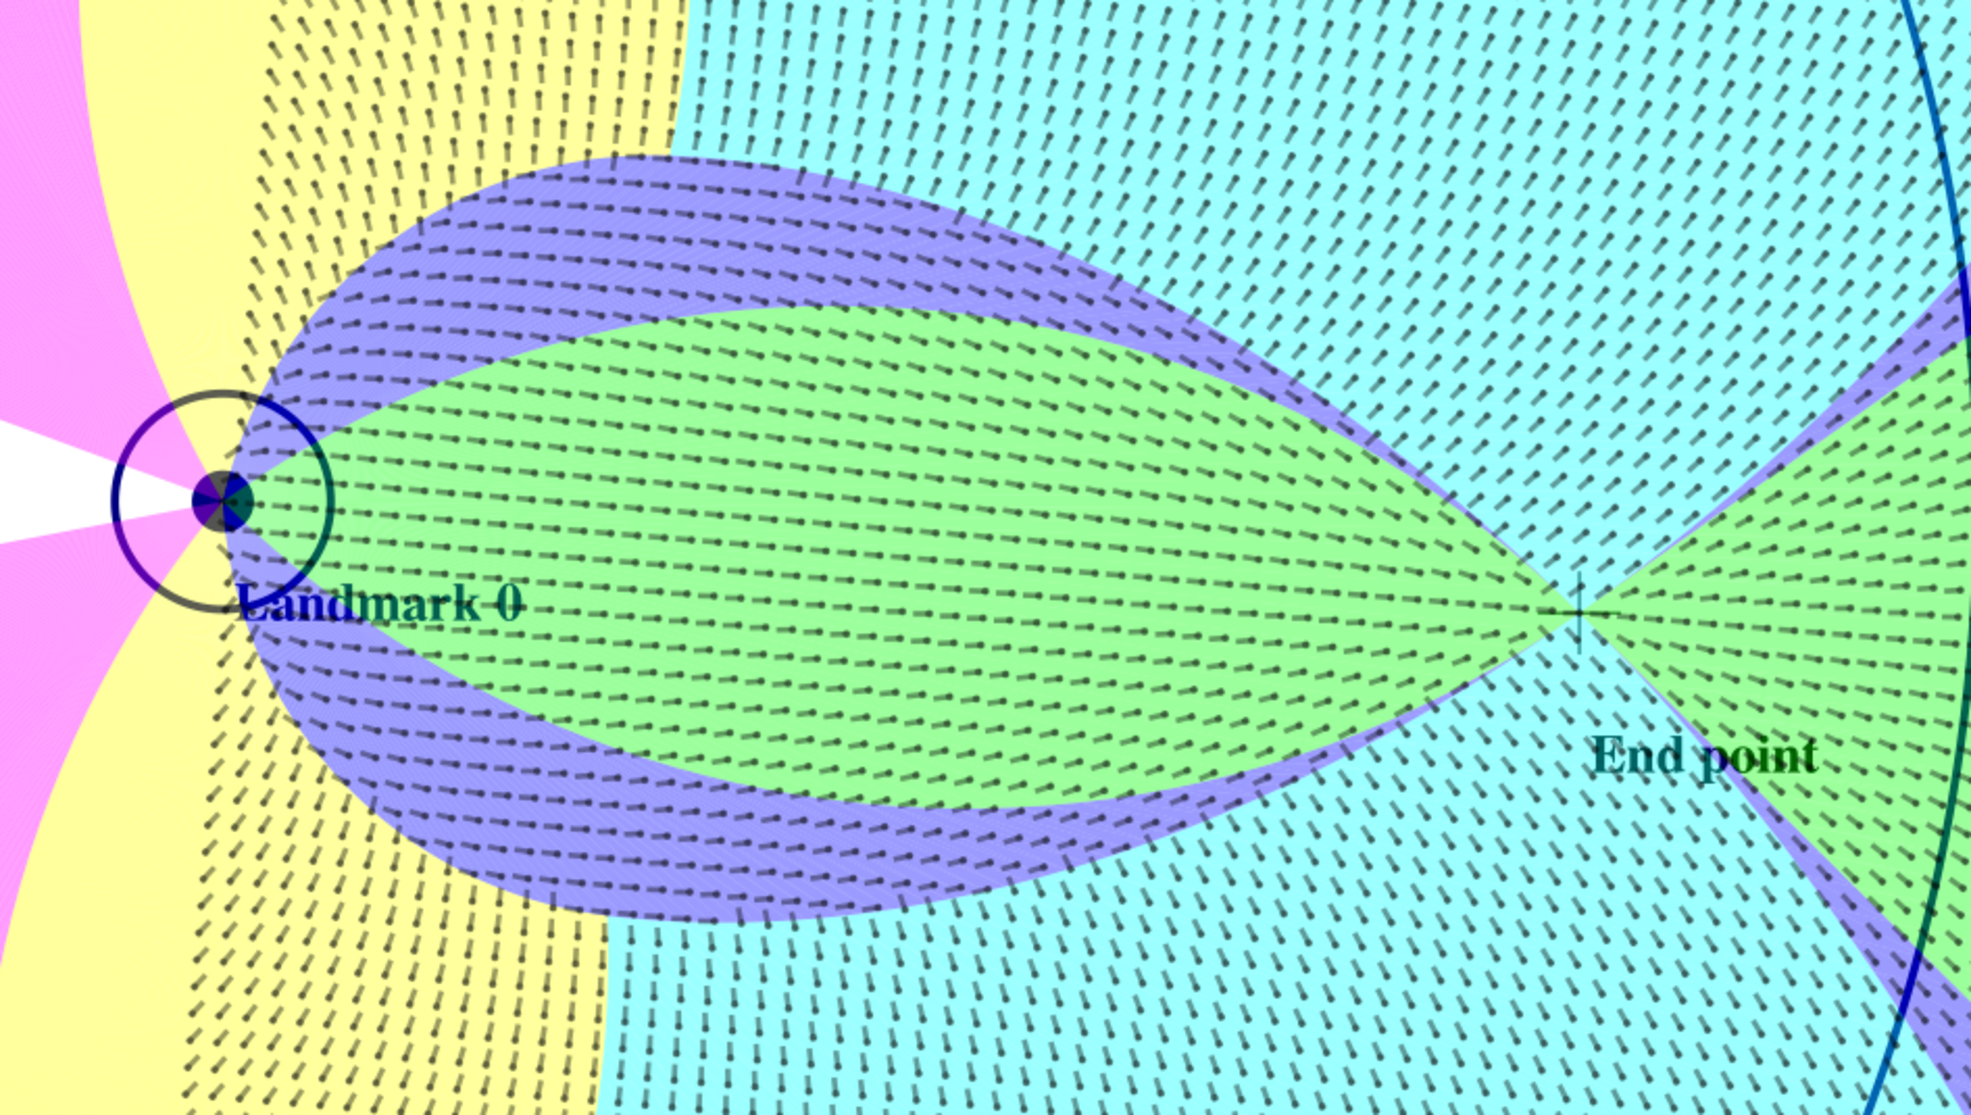
\includegraphics[scale=0.35]{Chap5-Visual-Planning/noLateral}
   \label{fig:fieldNoLateral}
   }
   %\hspace{15 mm}
 \subfigure[Motion direction field with lateral motions.]{
  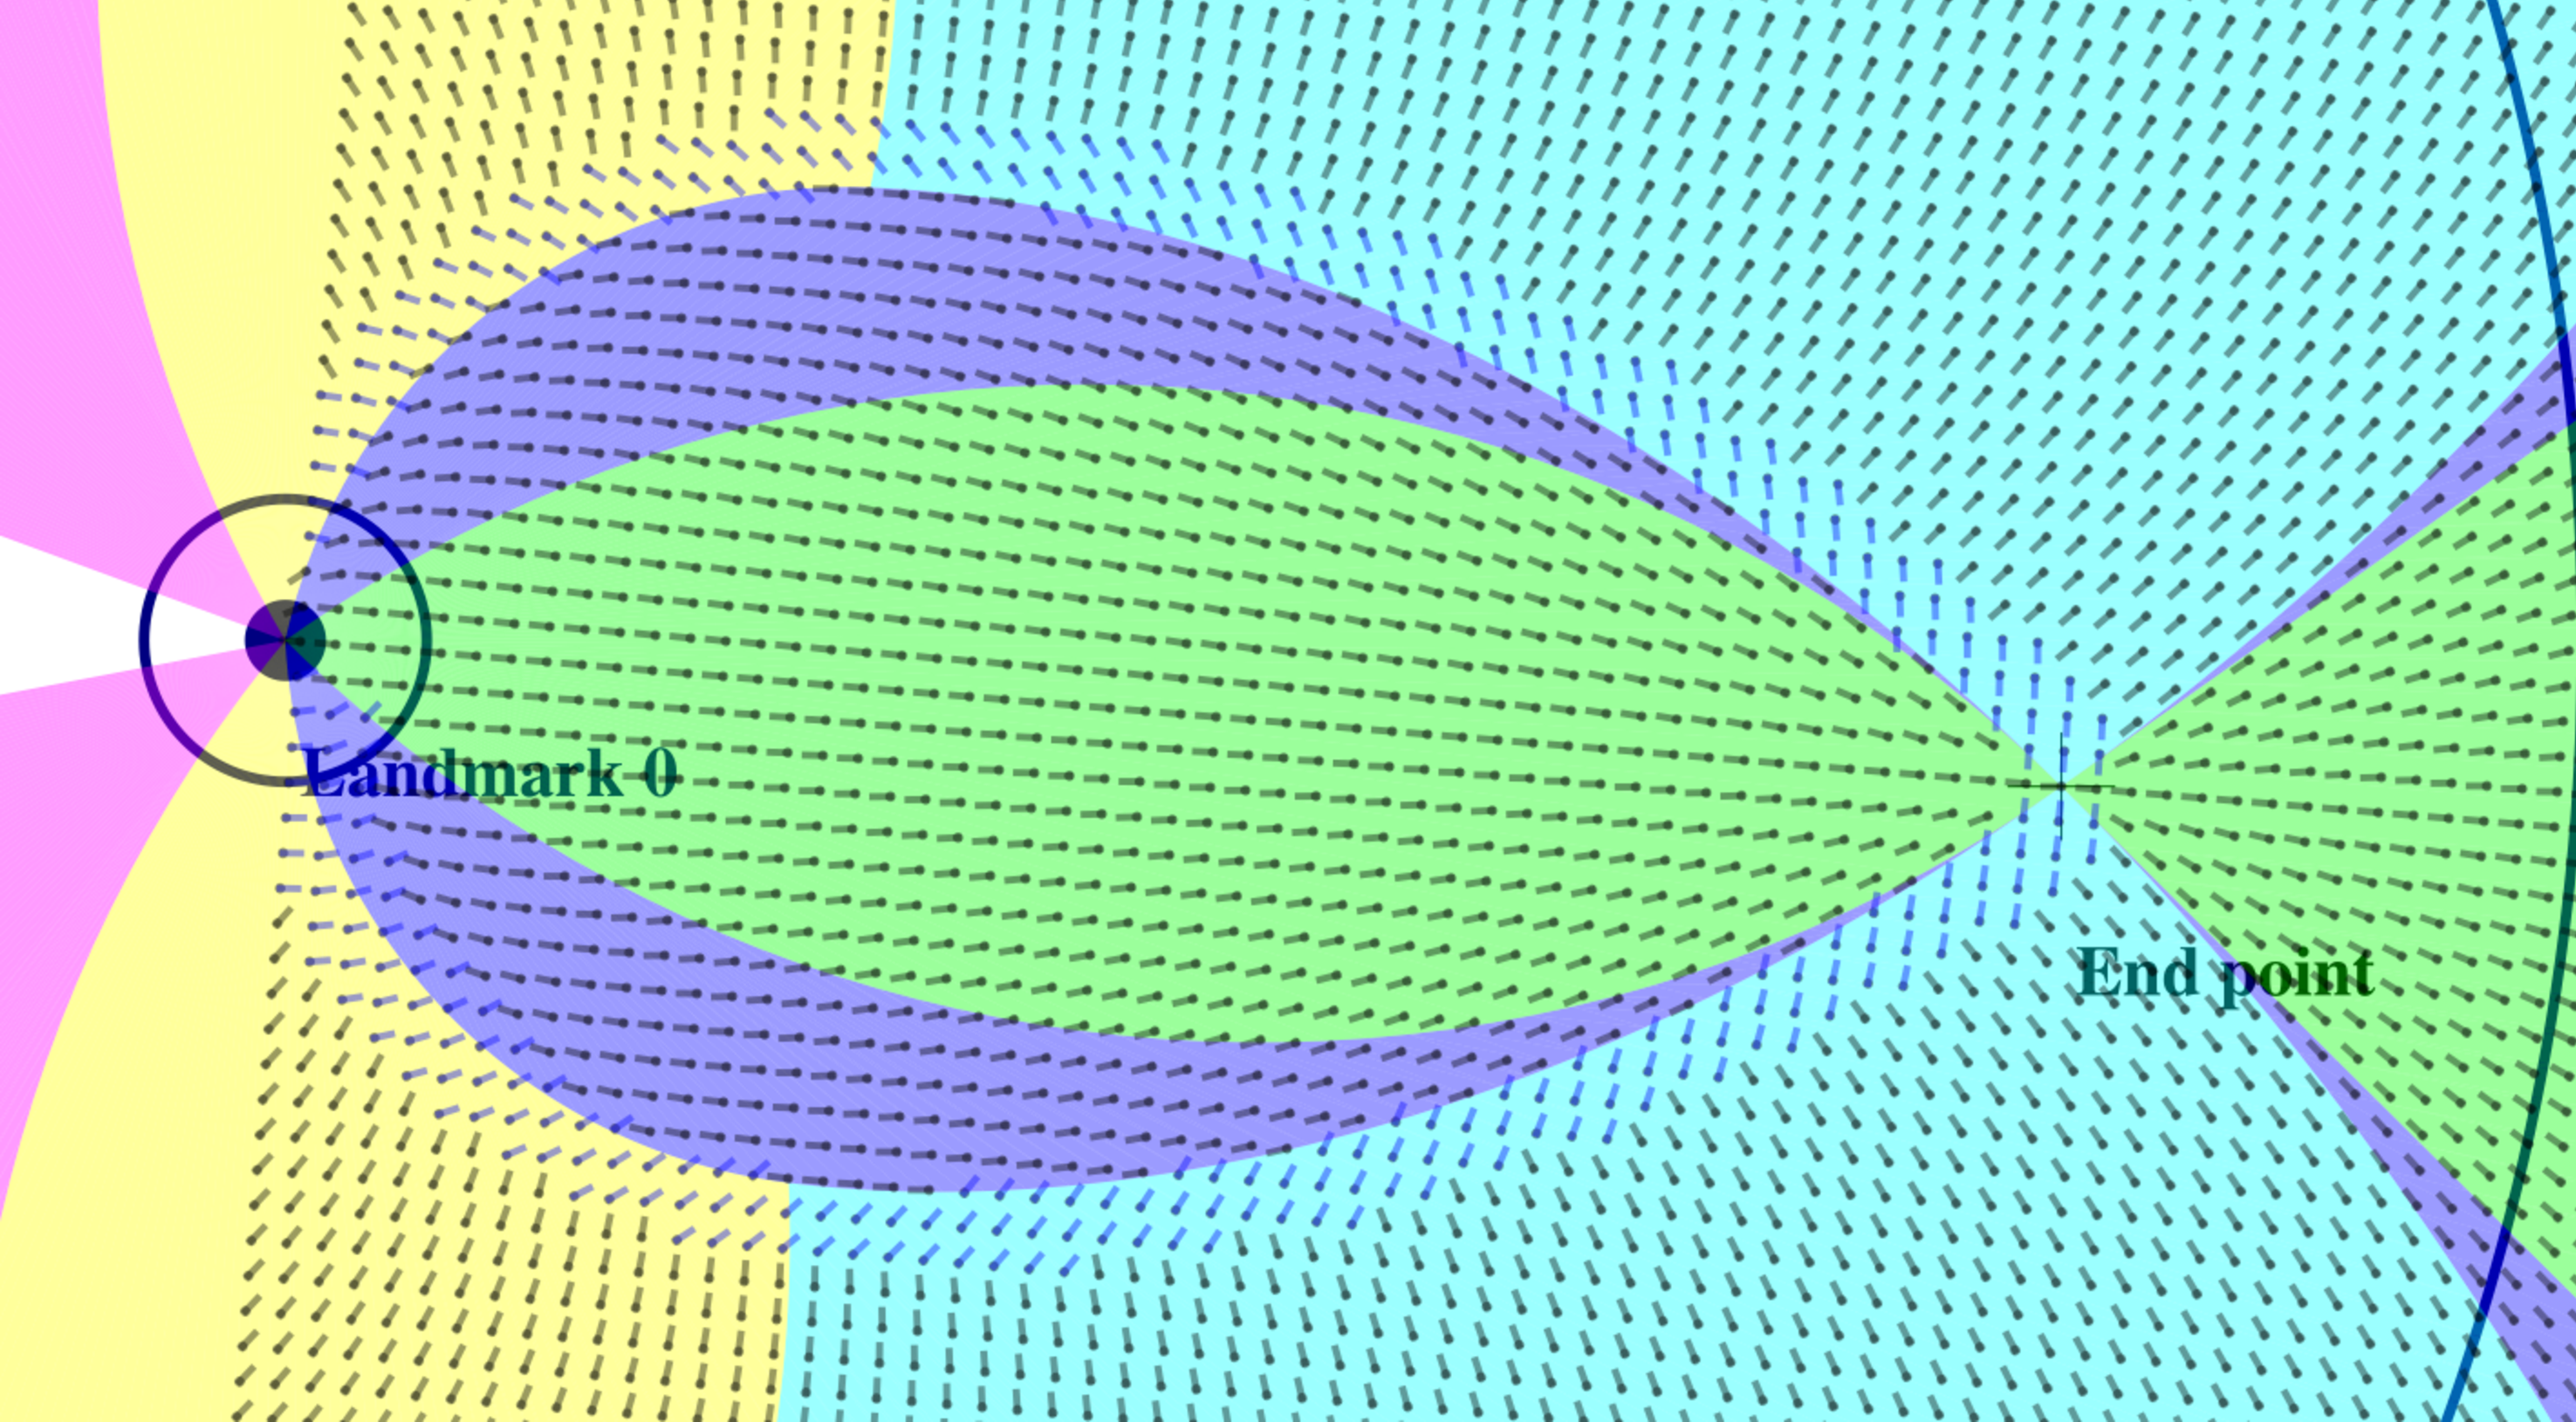
\includegraphics[scale=0.235]{Chap5-Visual-Planning/useLateral}
   \label{fig:fieldUseLateral}
   }
 \caption[]{Visualization of optimal motion directions $\theta^*(x,y)$. Both figures indicate the nature of optimal paths with the filling colors, and the tangent direction to the optimal curve all over a grid defined around the final point. In Fig.~\subref{fig:fieldNoLateral}, the field is computed directly from the primitives of~\citep{Salaris:2010}. The locus of in-site rotations is identifiable at the dark blue zone border. In Fig.~\subref{fig:fieldUseLateral}, the non-holonomy behavior close to this locus is replaced by lateral motions.\label{fig:field}}
\end{figure*}

\subsection{Using the optimal path synthesis within the MPC}

Instead of utilizing in the Equation~\ref{Eq:MinJerk}, a single, constant reference trajectory, defined by the plan computed from $p^s$ to $q^s$, and from which $(\dot{X}_{k+1}^{ref},\dot{Y}_{k+1}^{ref})$ would be evaluated, our idea is to use explicitly the mapping $\sigma$ described above. This way, we can adapt the path execution and find the shortest path to the next sub-goal from any point, not just from $p^s$. Even more, we can adapt to any change in the execution on the fly. As explained above, one can  associate to any $x,y$ the tangent $\theta^*(x,y)$ to the shortest path. One way to enforce the tracking of these shortest paths is to set as a reference velocity (supposing we are following a piece of curve with $v=1$) defined in the time horizon ($l>k$, where $k$ is the current time index):

$$
\begin{array}{ccc}
\dot{x}^{ref}_l =  \cos(\theta^*(x_l,y_l)) & \; & \dot{y}^{ref}_l =  \sin(\theta^*(x_l,y_l)) \\
\end{array}
$$

that depends (non-linearly) on $x_l,y_l$. The idea is to use these -- variable -- reference velocities inside the terms of the pattern generator QP. However, as this mapping is non-linear, a direct use would make us lose the QP form, that allows an efficient resolution of the problem. Because the mapping $\theta^*(x,y)$ has not always an analytic form we evaluate it numerically on a fine scale grid inside the zone of operation of the robot, as pre-computed values, and we also estimate numerically the partial derivatives $\frac{\partial \theta^*(x,y)}{\partial x},  \frac{\partial \theta^*(x,y)}{\partial y}$.

This way, we can approximate each of these reference velocities, at time position $l$ within the optimization time window, by performing a linearization of $\theta^*$  around a reference position $(x^0,y^0)$, i.e.,
$$
\begin{array}{ccc}
\theta^*(x_l,y_l) & \approx & \theta^*(x^0_l,y^0_l)  \\
& & + \frac{\partial \theta^*(x^0,y^0)}{\partial x} (x_l-x^0) + \frac{\partial \theta^*(x^0,y^0)}{\partial y} (y_l-y^0).
\end{array}
$$

Note that the linearization point $(x^0,y^0)$ is chosen in the aforementioned grid of pre-computed values $(\theta^*(x,y),\frac{\partial \theta^*(x,y)}{\partial x},  \frac{\partial \theta^*(x,y)}{\partial y})$, at the closest point to the first (current) CoM position. This grid is depicted in the background of Figs.~\ref{fig:steps6}, \ref{fig:field}, \ref{fig:steps10} among others. To simplify the notation, let us write
$$
\theta^0 \stackrel{\mbox{\tiny def}}{=}  \theta^*(x^0,y^0),\;
\frac{\partial \theta^0}{\partial x} \stackrel{\mbox{\tiny def}}{=} \frac{\partial \theta^*(x^0,y^0)}{\partial x},\;
\frac{\partial \theta^0}{\partial y} \stackrel{\mbox{\tiny def}}{=}  \frac{\partial \theta^*(x^0,y^0)}{\partial y}. 
$$


Then, we re-write the errors to the reference velocities at each time step $l>k$, as a linear function of $\dot{x}_l,\dot{y}_l,x_l,y_l$
$$
\left\{
\begin{array}{ccc}
\dot{x}_l-\dot{x}^{ref}_l & = & \dot{x}_l - v\cos(\theta^0)\\
&& + v\sin(\theta^0) \frac{\partial \theta^0}{\partial x}  (x_l-x^0)\\
&& + v\sin(\theta^0) \frac{\partial \theta^0}{\partial y}  (y_l-y^0),\\
\dot{y}_l-\dot{y}^{ref}_l & = & \dot{y}_l - v\sin(\theta^0_l)\\
&& - v\cos(\theta^0) \frac{\partial \theta^0}{\partial x}  (x_l-x^0)\\
&& - v\cos(\theta^0) \frac{\partial \theta^0}{\partial y}  (y_l-y^0),
\end{array}
\right.
$$ 

and by stacking the errors within the horizon window as in Eq.~\ref{Eq:PosCMHorizon}, we get the following 
linear relations

{\small
\begin{eqnarray}
\nonumber
 \dot{C}_x(k+1)  - \dot{C}_x^{ref}(k+1) & = &    \dot{C}_{x}(k+1) -   \dot{C}^{0}_x(k+1)  + A^0_{x} C_{x}(k+1)  + B_x^{0} C_{y}(k+1),\\
\nonumber
 \dot{C}_{y}(k+1) - \dot{C}_y^{ref}(k+1) & = &   \dot{C}_{y}(k+1) - \dot{C}^0_x(k+1) + A^0_{y} C_{x}(k+1) + B^0_{y}  C_y(k+1),\\
 \label{eq-velref-linear}
 \end{eqnarray}
}

where $A^0_{x},B^0_{x},A^0_{y},B^0_{y}$ are diagonal matrices collecting the terms $v\sin(\theta^0_l) \frac{\partial \theta^0_l}{\partial x}$ and alike. Then, the walking pattern generation is formulated exactly as in Eq.~\ref{Eq:MinJerk}, with the reference velocities given by Eq.~\ref{eq-velref-linear}, and with the optimization variable being $U(k)$,
%$U_{k} \stackrel{\mbox{\tiny def}}{=}  \left( (\dddot{C}_k^{x})^ \transpose, (X_{k}^{f})^ \transpose, (\dddot{C}_k^{y})^ \transpose, (Y_{k}^{f})^ \transpose \right)^{\transpose}$ 
leading to a canonical Quadratic Program (QP) similar to Eq.~\ref{Eq:QP}.

%{\scriptsize
%\begin{eqnarray}
%\nonumber
% \min\limits_{\dddot{C}^x_k,Z^x_{k+1},\dddot{C}^y_k,Z^y_{k+1}}  &&  \dfrac{\beta}{2} \left\| \dot{C}_{k+1}^{x}  - \dot{X}_{k+1}^{ref} \right\|^2 + \dfrac{\beta}{2} \left\| \dot{C}_{k+1}^{y}  - \dot{Y}_{k+1}^{ref} \right\|^2 \\
%\nonumber
%&& + \dfrac{\gamma}{2} \left\| Z^{x_{ref}}_{k+1} - Z^x_{k+1} \right\|^2 + \dfrac{\gamma}{2} \left\| Z^{y_{ref}}_{k+1} - Z^y_{k+1} \right\|^2 \\
%&& + \dfrac{\alpha}{2} \left\| \dddot{C}_{k}^{x}  \right\|^2 + \dfrac{\alpha}{2} \left\| \dddot{C}_{k}^{y} \right\|^2,
%\label{eq-main-qp}
%\end{eqnarray}
%}

% that can be expressed in terms of $U_{k} \stackrel{\mbox{\tiny def}}{=} \left( (\dddot{C}_k^{x})^ \transpose, (Z_{k+1}^{x_{ref}})^ \transpose, (\dddot{C}_k^{y})^ \transpose, (Z_{k+1}^{y_{ref}})^ \transpose \right)^{\transpose}$ by using Eq.~\ref{eq-velref-linear}, into a canonical Quadratic Program (QP) similar to Eq.~\ref{Eq:QP}.

Non-linear constraints arise from the CoP position to be included in the support polygon. In this case, we set the robot and feet orientations as specified in next section and include the computed values into the QP.

\subsection{Control of the rotation angle}
In order for the robot to be oriented with the tangent to the optimal path, $\theta^0$, we use a decoupled approach in a very similar way as what we already described in Section~\ref{Chap:Locomotion-Control} for the control of the rotation angles of the trunk and the feet~\citep{HerdtIROS2010}. With this formulation, we also mantain the QP form. Hence, in a first stage, we optimize the orientations in the MPC time window by  

\begin{eqnarray}
\nonumber
 \min\limits_{\dddot{C}_{\theta}(k),\dddot{F}_{\theta}(k)}  &&  \dfrac{\beta}{2} \left\| C_{\theta}(k+1) - \theta^{0} \right\|^2 + \dfrac{\gamma}{2} \left\| F_{\theta}(k+1) - \theta^{0} \right\|^2 \\
\nonumber && + \dfrac{\alpha}{2} \left\| \dddot{C}_{\theta}(k+1) \right\|^2 + \dfrac{\alpha}{2} \left\| \dddot{F}_{\theta}(k+1) \right\|^2,
\end{eqnarray}

and then in a second stage, we introduce these angles as constant in the main QP (Eq.~\ref{Eq:MinJerk}). This approach gives us the advantage of introducing constraints like maximum rotation between both feet, between feet and trunk and also a rotation limit to keep the visibility of the landmarks.

%\subsection{Refinement of the angular position}

%\textcolor{blue}{JB:} Will we do something about that?: the idea would be to do a second pass where the $\theta^0$ would be re-evaluated.

%\textcolor{blue}{MG:} You meant the linearization points right, is it still necesary after the clarification?

%=============================================================================================================================================================

\section{Including holonomic behavior}
\label{sec:includingholonomic}

Handling holonomic and non-holonomic behaviors together during locomotion has been previously been discussed in \citep{MombaurHumanoids2008} in a context of motion planning.

One of the most visible disadvantages of the optimal non-holonomic paths given from~\citep{jib-IJHR2010} is the presence of in-site rotations, that are not efficient in terms of footsteps number.
One solution is to use a different formulation of the cost function using weights according to the robot direction and control the head.
But including this vision based control in Eq.~\ref{Eq:MinJerk} is incompatible with a QP formulation.
A strategy we propose here is to take advantage of the fact that the set of points where in-site rotations occur is very well defined geometrically in the plane, as a direct consequence of the synthesis from~\citep{Salaris:2010}. As illustrated in Fig.~\ref{fig:fieldNoLateral}, it is the outer boundary of the partition zone where the shortest paths have to be done as line segments followed by spirals, i.e. the dark blue region of the figure. This curve is made of two parts~\citep{Salaris:2010}, one arc of circle and one piece of logarithmic spiral. Hence, we propose to perform the following: for all points inside the partition regions in contact with this locus, we evaluate its distance in terms of the primitive to be done to reach this locus and modify the reference velocities as follows. 

If the robot is far from the locus of in-site rotations, then the path to follow is continuously derivable and goes either forwards or backwards; in that case, we use the ``non-holonomic behavior'' as described in Section~\ref{sec:reftrajectories}, with the robot orientation controlled to stay close to $\theta^*(x_l,y_l)$,
$$
\begin{array}{c}
\dot{x}^{ref}_l  =  \cos(\theta^*(x_l,y_l)) \;,\; \dot{y}^{ref}_l  =  \sin(\theta^*(x_l,y_l)), \\
\end{array}
$$

and if the robot configuration is close to this locus, then we use instead lateral motions, with orientation $\phi(x_l,y_l)+\pi$, where $\phi(x_l,y_l)=\arctan\frac{y_l}{x_l}$ is the polar angle of $(x_l,y_l)$,
$$
\begin{array}{c}
\dot{x}^{ref}_l  =  -\varepsilon\sin(\phi(x_l,y_l)) \;,\; \dot{y}^{ref}_l  =  \varepsilon\cos(\phi(x_l,y_l)),  \\
\end{array}
$$

where $\varepsilon =\pm1$ in function of the relative position of the goal to reach with respect to the evaluated point. 

In Fig.~\ref{fig:fieldUseLateral}, we illustrate this modification by drawing the lateral motion field with blue arrows, together with the ``non holonomic'' field ``far'' from the locus of in-site rotations. 

%=============================================================================================================================================================
\section{Results}

%=============================================================================================================================================================

In this section, we present three experiments. In the first one, we test the performance of our approach in the absence of localization uncertainty, and with only non-holonomic motion. In the second one, we introduce localization uncertainty. In the last one, we present an improvement to the border behavior with the possibility of holonomic motion. The three experiments have the same set-up, with initial position in $(0.5,2.5)$, landmark position in $(0,0)$ and final position in $(-3,0)$. We chose this trajectory because it makes the robot pass through several regions of the partition and illustrates the border behavior which is one of the problems we found.

In Fig.~\ref{fig:steps6}, we depict the performance in perfect and noiseless conditions. We see that using the planner vector field, for driving the robot to the goal produces smooth and stable trajectories of the CoM. However, in real conditions, the robot will not perform the control exactly e.g., because of sliding with the floor. Moreover the robot needs a localization system which will be inherently noisy. To model this situation, we perturbed the current position of the CoM with white gaussian noise $\sim \mathcal{N}(0,\sigma^2)$ in each coordinate with $\sigma = 0.2$m for translation and with $\sigma = 10$ degrees for the orientation.

\begin{figure}[ht]
\centering
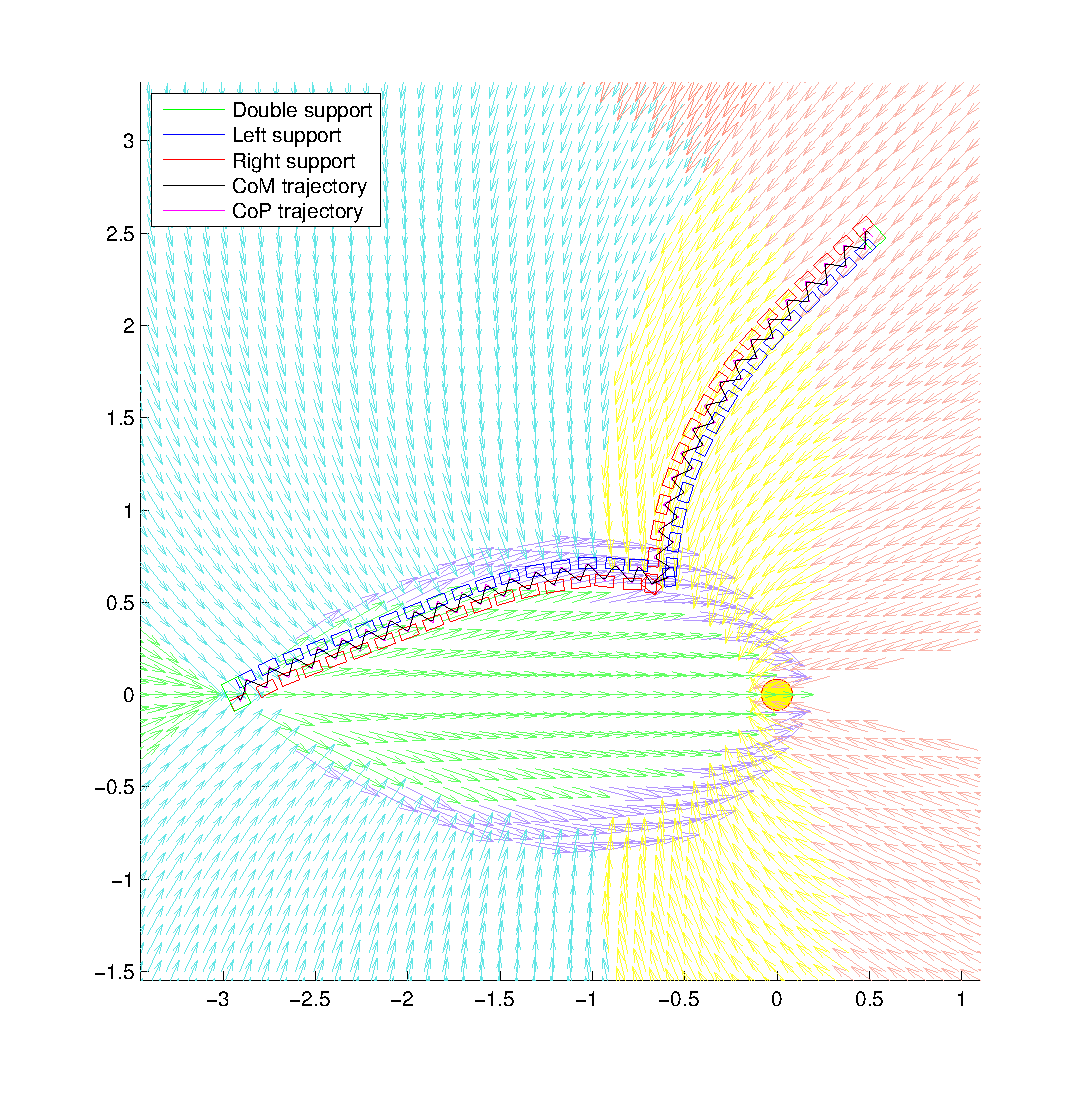
\includegraphics[scale=0.8]{Chap5-Visual-Planning/steps6.pdf}
\caption{Vector fields generated by optimal trajectories planned with visibility constraints for a non-holonomic robot~\citep{Salaris:2010}. To each color is associated a family of global paths that reach the goal (at $(-3,0)$) according to the current configuration of the robot while keeping the landmark (yellow disk) visible at all times. The footsteps, CoM and CoP trajectories for the humanoid robot are all depicted as indicated in the upper box.}
\label{fig:steps6}
\end{figure}

In Fig. \ref{fig:steps10}, we show the behavior in that situation. We can still appreciate a smooth trajectory in the regions far from the border of the dark blue region of the partition, where the vector field is smooth. We also notice the good behavior of the orientation angle mainly because the QP formulation controls it. The main problem of this approach also appears: The discontinuities in the partition regions in which an in-site rotation occurs. Hence, the robot may perform unnecessary maneuvers, involving in-site rotations, which is far from optimal in the case of human walking (Fig.~\ref{fig:steps10zoom}). Moreover, in-site rotations cause high rotation speeds of the feet (Fig.~\ref{fig:velocities10}), which is not desirable from a balance point of view.

\begin{figure}[ht]
\centering
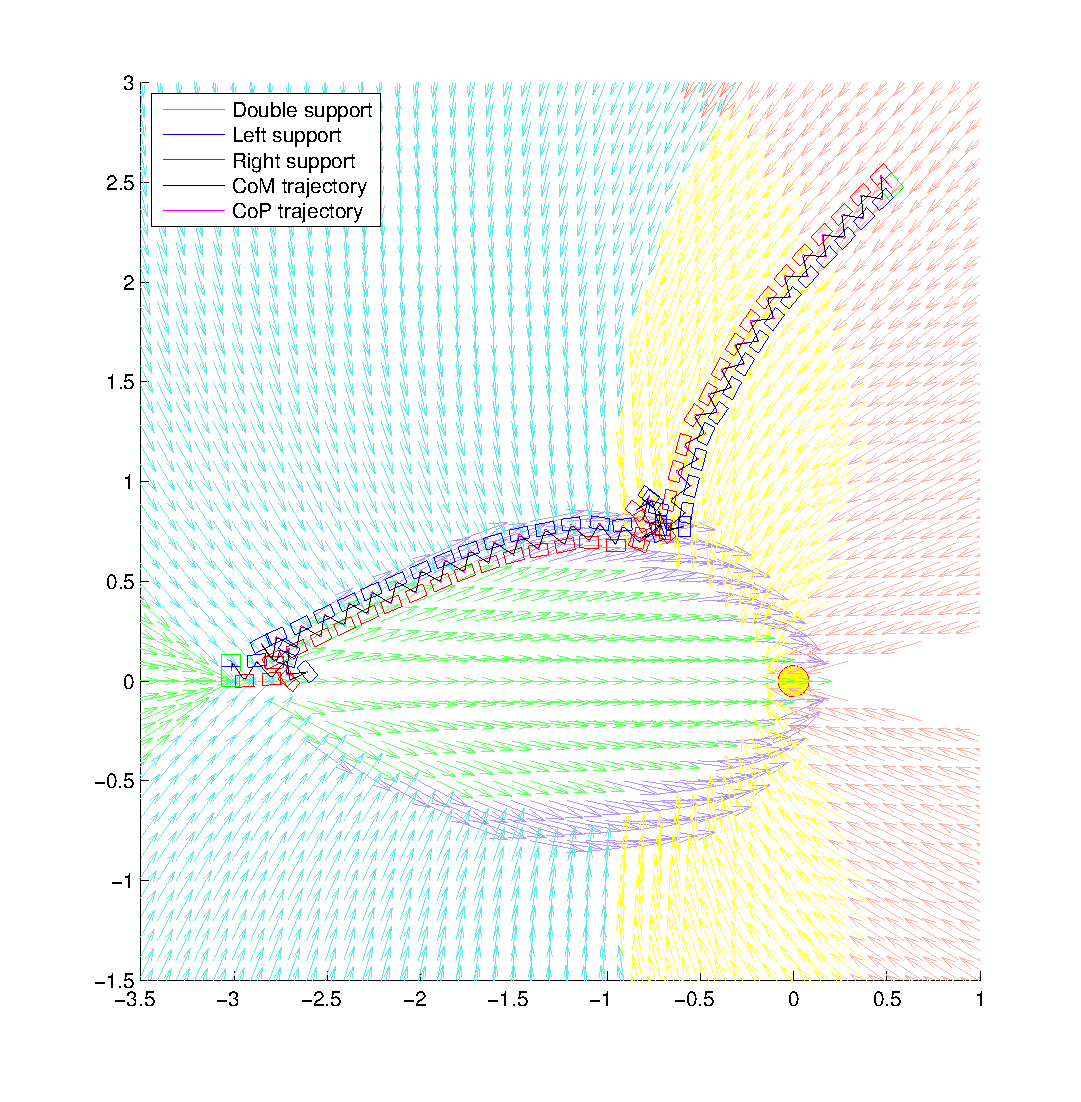
\includegraphics[scale=0.8  ]{Chap5-Visual-Planning/steps10.pdf}
\caption{If the control is not followed well and if we use an imperfect localization system, problems may arise in the borders of the partition, in case of relying on purely non-holonomic behaviors.}
\label{fig:steps10}
\end{figure}

\begin{figure}[ht]
\centering
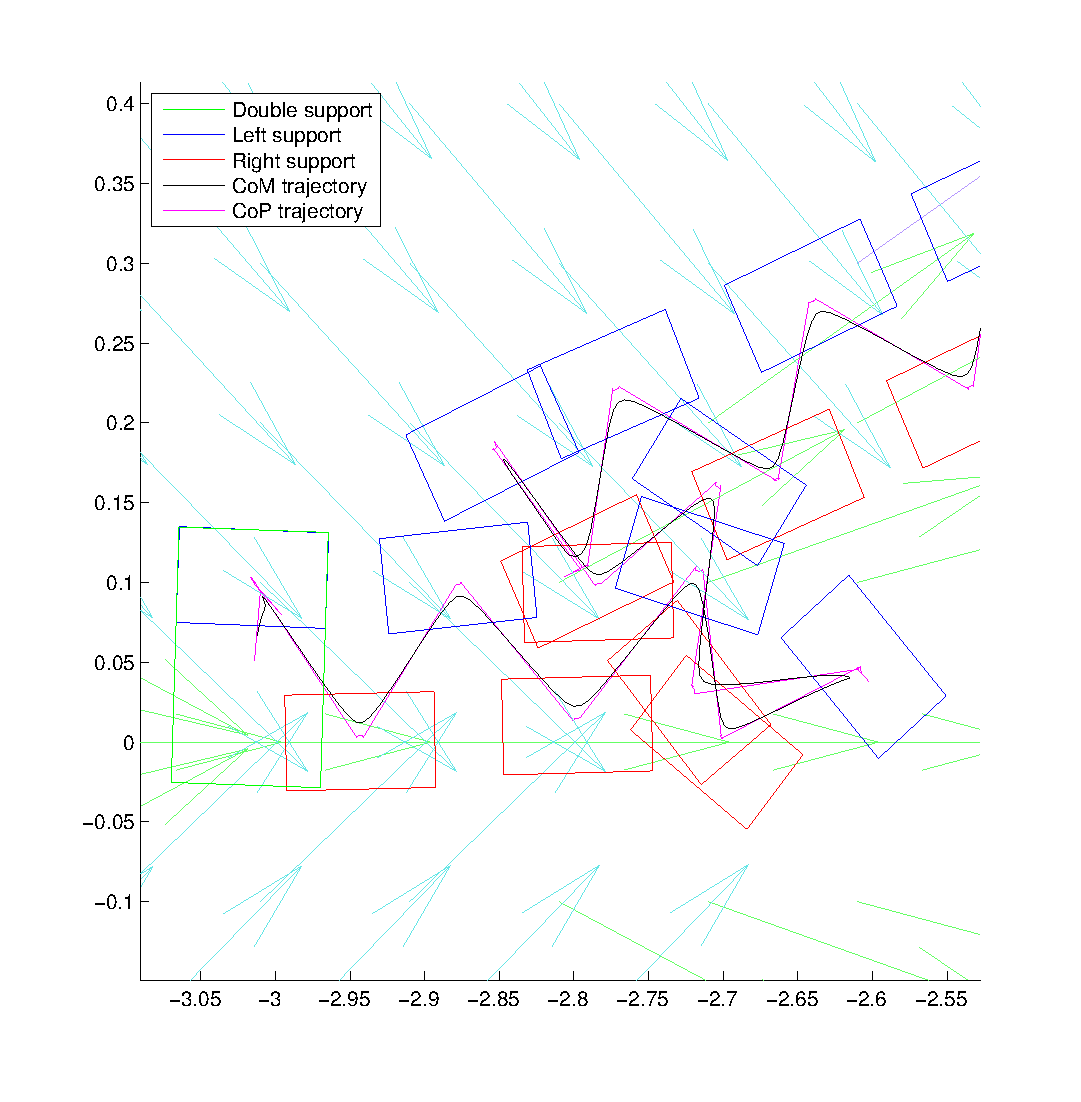
\includegraphics[scale=0.55]{Chap5-Visual-Planning/steps10zoom.pdf}
\caption{Zoom on Fig.~\ref{fig:steps10}, close to $(-3,0)$. As the robot compensates sliding and localization errors non-holonomically, more in-site rotations occur.}
\label{fig:steps10zoom}
\end{figure}

\begin{figure}[ht]
\centering
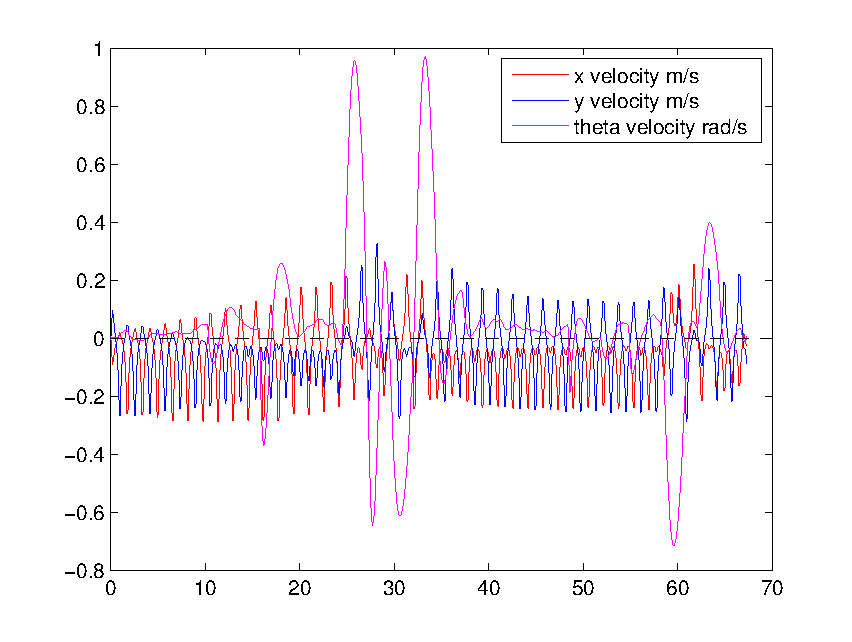
\includegraphics[scale=0.7  ]{Chap5-Visual-Planning/velocities10.pdf}
\caption{Velocities profile for the trajectory depicted in Fig.~\ref{fig:steps10}. The overshoots in the angular velocity are caused by the in-site rotations at the border of the dark blue region of the partition.}
\label{fig:velocities10}
\end{figure}

To address the aforementioned problem, we present the results of the improvement introduced in Section~\ref{sec:includingholonomic}. In Fig.~\ref{fig:steps11}, we perform the same trajectory but by introducing the possibility of holonomic motion in the region where in-site rotations would be necessary. The robot is not performing in-site rotations anymore, but a mixture of holonomic and non-holonomic motions, depending on its position with respect to the border. We can appreciate better the transition between non-holonomic and holonomic motions in Fig. \ref{fig:steps11zoom}. %Finally in Fig. \ref{fig:velocities11} we can see the reduction of the angular velocity necesay to perform the motion.

\begin{figure}[ht]
\centering
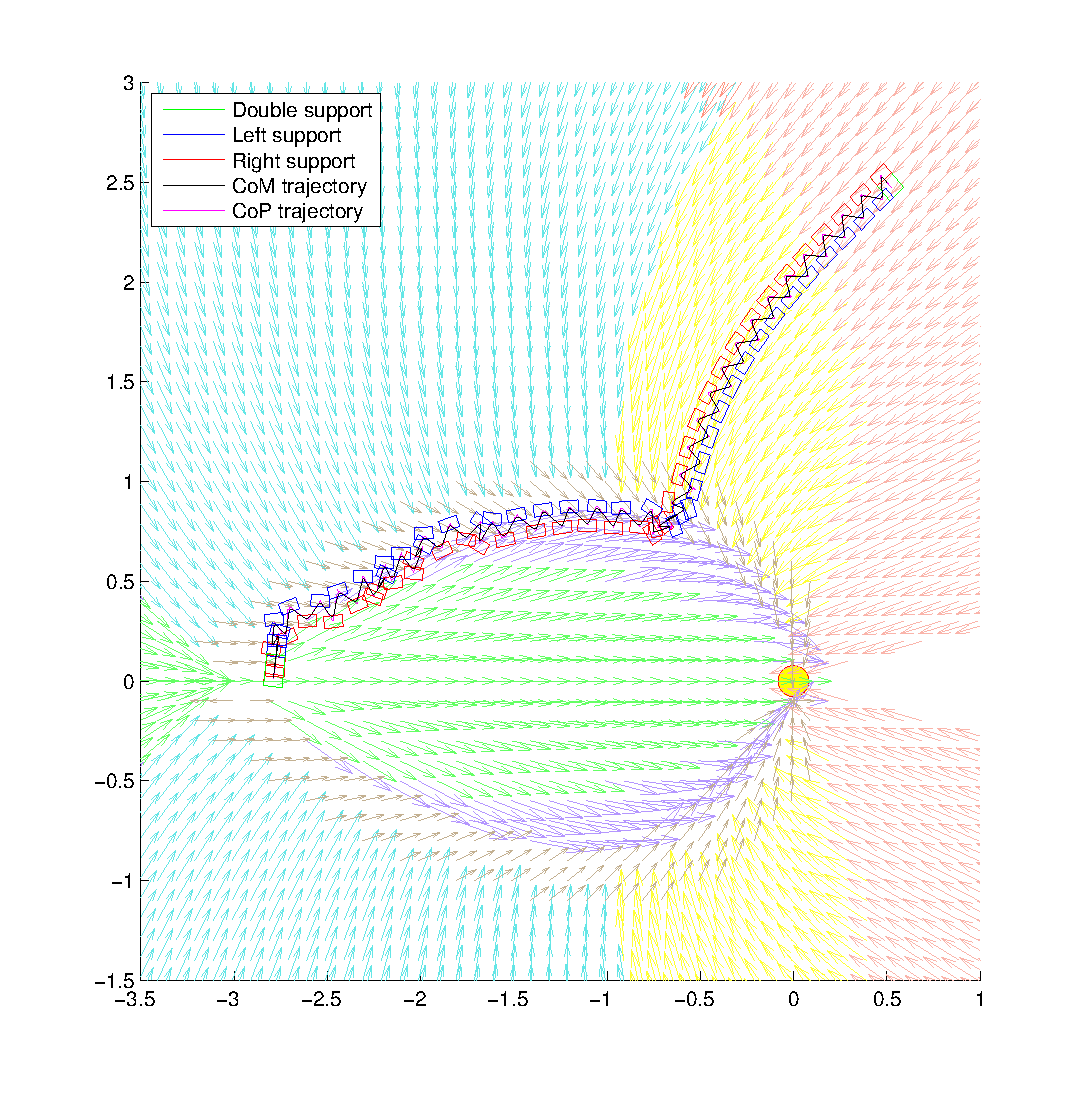
\includegraphics[scale=0.8  ]{Chap5-Visual-Planning/steps11.pdf}
\caption{Trajectory with holonomic motion made possible. Lateral motion is allowed in the khaki vector field in the orientation discontinuity region.}
\label{fig:steps11}
\end{figure}

\begin{figure}[ht]
\centering
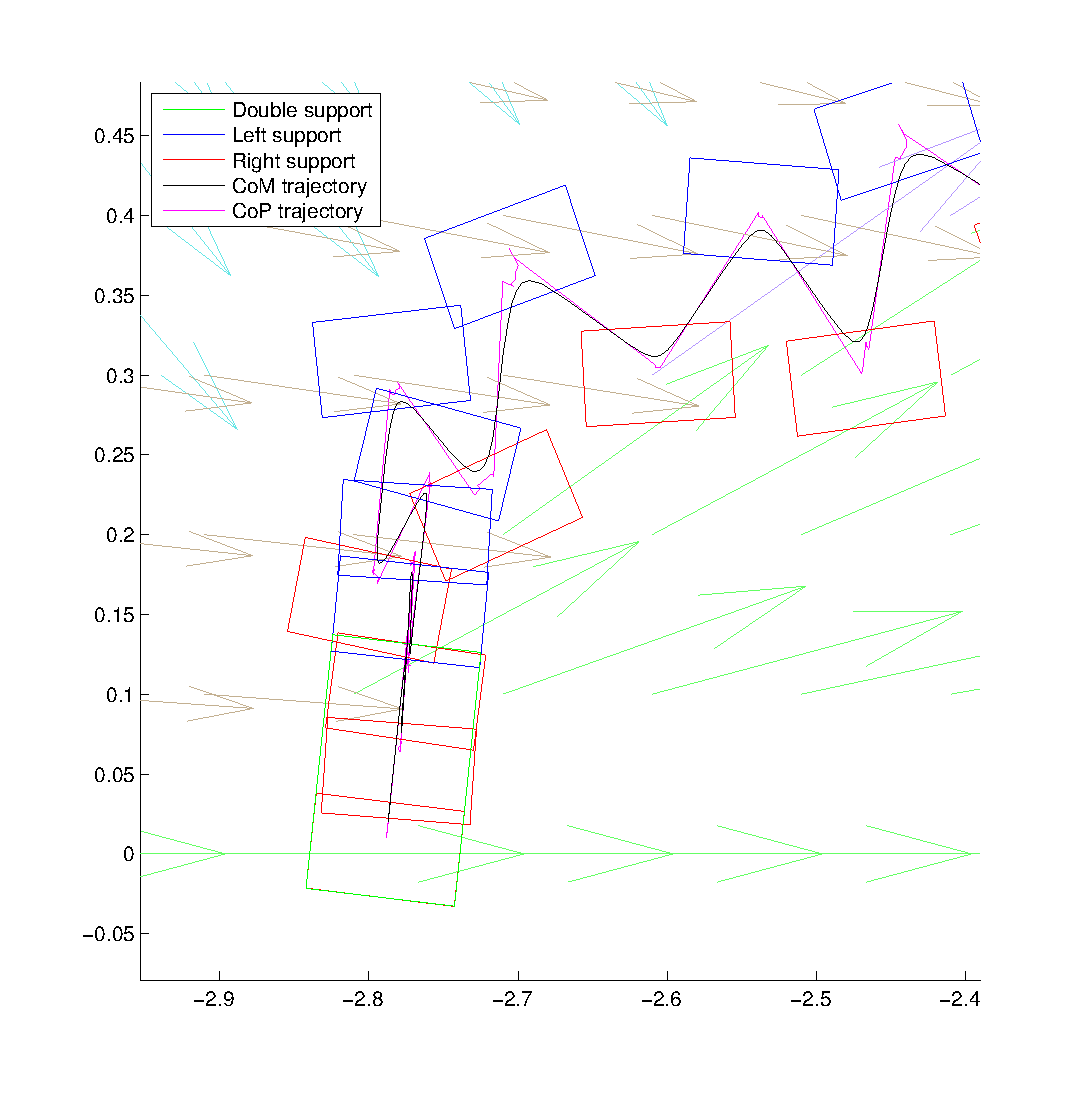
\includegraphics[scale=0.55]{Chap5-Visual-Planning/steps11zoom.pdf}
\caption{Transition between non-holonomic and holonomic controls. Moving sideways is much more efficient for such a trajectory to reach the goal.}
\label{fig:steps11zoom}
\end{figure}

%\begin{figure}
%\centering
%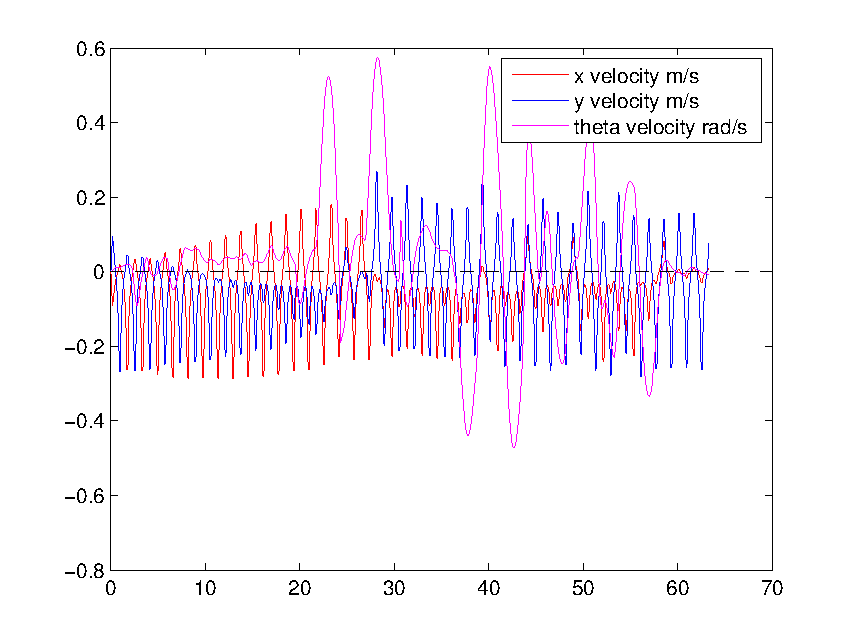
\includegraphics[scale=0.4]{velocities11.pdf}
%\caption{Velocities profile for the trajectory of the figure \ref{fig:steps11}. We can see that those velocities are in good limits and provide a stable walking. }
%\label{fig:velocities11}
%\end{figure}

%=============================================================================================================================================================
\section{Conclusion}
\label{sec:conclusion}
%=============================================================================================================================================================

In most of the current literature, the link between planning and locomotion control has been given by footsteps. In this paper, we propose a novel approach that uses directly the optimal motion synthesis derived from the planner to the control system without going through footsteps but instead by computing them within the Walking Pattern Generator. With this approach, we can drive the robot to a desired goal by using an external planner, not necessarily the one used in this paper. We tested our approach simulating real situations such as situations with localization noise and sliding of the feet. We have also tried to make the walking pattern more efficient by introducing the possibility of using holonomic motion. Our next objective is to test the approach introduced in this paper on the HRP-2 platform.


% 3D reconstruction
\chapter{Stereo Reconstruction of Dense Surfaces to Walk on Rough Terrain} 
\label{Chap:3DReconstruction}

As we stated in figure \ref{Fig:GeneralDiagram} computer vision can be introduced (from hight to low level) in planning level, pattern generator level or whole-body motion level. In this chapter we will addresse the introduction of computer vision in the lowest level of robot motion generation: The Generalized Inverse Kinematics (GIK).

\section{The Stack of Tasks}
% ~~~~~~~~~~~~~~~~~~~~~~~~~~~~~~~~~~~~~~~~~~~~~~~~~~~~~~~~~~~~~~~~~~~~~~~~~~~~~

The Stack of Tasks (SoT) is a system that implements the Generalized Inverted Kinematics (GIK). GIK is extensively used to do low level control in highly redundant robots. The SoT uses the notion of task and, moreover the notion of tasks priority. 

Given the current value of the features $\mathbf{s}_i$ and the desired ones $\mathbf{s}^{*}_i$, a task is defined as,

$$
\mathbf{e}_i = \mathbf{s}_i - \mathbf{s}^{*}_i,
$$

The relation between the task and the the articular positions of the robot $\mathbf{q}$ is given by

$$
\dot{\mathbf{e}}_i = \mathbf{J}_i \dot{\mathbf{q}}_i,
$$

with $\mathbf{J}_i = \dfrac{\partial \mathbf{e}_i}{\partial \mathbf{q}} $. The control law which gives an exponential decay is,

$$
\dot{\mathbf{q}}_i = - \lambda \mathbf{J}^{+}_i \mathbf{e}_i.
$$

At dynamic level, the acceleration must be used, in this case the relation is given by,

$$
\ddot{\mathbf{e}}_i = \dot{\mathbf{J}}_i \dot{\mathbf{q}} + \mathbf{J}_i \ddot{\mathbf{q}}.
$$

\section{Walking on Rough terrain}
% ~~~~~~~~~~~~~~~~~~~~~~~~~~~~~~~~~~~~~~~~~~~~~~~~~~~~~~~~~~~~~~~~~~~~~~~~~~~~~

In \citep{RamosIJHR2013} a porposal to walk on rough terrain was presented. It uses an inverse dynamics approach and a 3D reconstruction system to implement a compliant walking scheme. The inverse dynamics control scheme relying on a quadratic programming optimization solver is used to let each foot go from its initial to its final position, controlling also the center of mass and the waist. A 3D model reconstruction of the ground is obtained through the robot cameras located on its head as a stereo vision pair. The model allows the system to know the ground structure where the swinging foot is going to step on. Thus, contact points can be handled to adapt the foot position to the ground conditions.

The inverse dynamics scheme is based in tree tasks: (i) a task for tracking the position of the CoM given by the Pattern Generator, (ii) a task to partially track the waist trajectory, this taks controls the height of the waist as well as its orientation and, (iii) an interpolation task, this task takes the swinging foot from its initial position to its desired final position, the foot reacts in a compliant way if a contact is detected before arriving to the final position on the ground.

The contact points detection is done using a 3D model of the floor in front of the robot. This 3D model comes from a Stereo reconstruction system which will ve explained in more details in next section.

\section{Stereo reconstruction}

To perform the dense reconstruction of the floor surface in front of the robot, we rely on a real-time approach similar to KinectFusion algorithm proposed in~\citep{Newcombe2011}. This approach, originally developed for a RGB-D sensor, models 3-D surfaces as zero-valued level sets of functions defined over the workspace volume. These functions are referred to as truncated signed distance function (TSDF) and they are built incrementally, by integrating the depth measurements the sensor provides, frame after frame. TSDF are defined in the 3D space, and their value is the signed distance to the closest obstacle. Here, we extend this approach, initially proposed for RGB-D depth data, to disparity data generated from a stereo head. Although the stereo data is noisier than the one from RGB-D sensors, it is a passive sensor and can be used outdoors in sunlight conditions.


Consider, as in the previous sections, that $k$ is a discretized time index. The idea is to update a mathematical representation of the surface through a volumetric TSDF model (defined over a 3D grid), referred to as $F_k$. The basic steps for integrating one new set of disparity measurements at time $k$, to update $F_k$ and the corresponding surface, are the following ones: (i) Filter the raw depth measurements generated from the stereo head, $D_k$; here we used bilateral filtering for that purpose; (ii) From these filtered measurements and the prediction of the estimated surface at the previous step, estimate the transformation between the measured surface and the predicted one using the iterative closest point algorithm (ICP) and update the camera pose; (iii) Compute a volumetric grid formed from ``local'' TSDF values $F_{D_k}$, to which confidence weights $W_{D_k}$ are associated, and integrate them into the global volumetric grid $\{F_k,W_k\}$; (iv) Predict a new surface for the next iteration by using ray-casting over the zero-crossings of the fused global volumetric grid $\{F_k,W_k\}$. 

To use this algorithm with stereo data and generate local data $D_k$, a disparity map from a pair of rectified images is estimated, from which the depth map $D_k$ is derived, supposing the stereo rig is completely calibrated. The literature of algorithms that estimate disparity maps is huge, but since a real time one is needed for this application, the one proposed in~\citep{Geiger2010} has been used. This algorithm estimates a piece-wise disparity map using an initial sparse disparity map of high textured points as vertices that define a triangulation of the image. Then, the dense disparity map of each sub-region is estimated by using the initial, sparse disparity map as a prior in a probabilistic scheme. The steps of the reconstruction process are illustrated in Fig.~\ref{Fig:Reconstruction1}

\subsection{Pre-processing}
As mentioned above, it is necesary to apply a bilateral filter to the raw depth map to smooth it preserving the borders.
Then we project the pixel $\mathbf{u}$ to obtain a 3D the point $\mathbf{p}$. With the projection of all the pixels, we generate a vertex map,

\begin{equation}
 \mathbf{V}_k(\mathbf{u}) = D_k(\mathbf{u})\mathbf{K}^{-1}(\mathbf{u}).
\end{equation}

Since the depth meassurements is a regular map, we can compute the normal vectors $\mathbf{N}_k(\mathbf{u})$ using the neighbours.



\subsection{Reconstruction}
The core of this algorithm is the computation and fusion of volumetric grids (i.e., the third step mentioned above). For a 3D point $\mathbf{p}$ expressed in the global frame $g$, its value in the current local volumetric grid $\{F_{D_k},W_{D_k}\}$ is computed as

$$
\left\{
\begin{array}{ccc}
F_{D_{k}}(\mathbf{p}) &=& \Psi (\lambda^{-1} \left \| \mathbf{t}_{g,k} - \mathbf{p}\right \| - D_k(\mathbf{x})), \\
W_{D_{k}}(\mathbf{p}) &\propto& \cos(\theta)/D_{k}(\mathbf{x}),
\end{array}
\right.
$$

with
$$
\Psi (\eta) =
\left \{
\begin{array}{cc}
\min(1,\frac{\eta}{\mu}) ~\text{sgn}(\eta) & \text{iff} ~ \eta \geq -\mu \\
\mbox{ null } & \mbox{ otherwise }
\end{array}
\right. , ~
\lambda = \left \| \mathbf{K}^{-1} [\mathbf{x}^\top 1]^\top \right \|,~
%\lambda = \left \| \mathbf{K}^{-1} \left[ \begin{matrix} \mathbf{x} \\ 1 \end{matrix} \right] \right \|,
$$

$\mu$ being a truncation distance (parameter of the algorithm), $\mathbf{x} = \pi([\mathbf{K},\mathbf 1] T^{-1}_{g,k} \mathbf{p}) \in \mathbb{R}^2$ being the image projection of $\mathbf p$. $\mathbf{K}$ is the $3\times 3$ matrix of intrinsic parameters of the camera, $\pi$ is the projection operator, $T_{g,k} = \left[ \begin{matrix} \mathbf{R}_{g,k} & \mathbf{t}_{g,k} \\ 0 & 1 \end{matrix} \right]$ the pose of the camera, at time $k$, in the global frame $g$, and $\theta$ the angle between the associated pixel ray direction and the surface normal.

The global volumetric grid at time $k$ is formed by the weighted average of all individual volumetric grids up to $k-1$. It can be shown that the optimal grid can be obtained incrementally using a simple point-wise on-line weighted average,

\begin{eqnarray*}
 F_k(\mathbf{p}) &=& \frac{W_{k-1}(\mathbf{p}) F_{k-1}(\mathbf{p}) + W_{D_{k}}(\mathbf{p}) F_{D_{k}}(\mathbf{p}) }{ W_{k-1}(\mathbf{p}) + W_{D_{k}}(\mathbf{p}) }, \\
 W_k(\mathbf{p}) &=& W_{k-1}(\mathbf{p}) + W_{D_{k}}(\mathbf{p}).
\end{eqnarray*}

\subsection{Surface prediction}
With the latest reconstruction we can compute a dense surface prediction by rendering the surface at the zero level of the TSDF on a virtual camera with the current estimation of $T_{g,k}$. This process will give us an estimated vertex and normal maps $\hat{\mathbf{V}}_k$ and $\hat{\mathbf{N}}_k$ that ww will use in the camera pose estimation.
The vertex map is predicted by marching each ray $T_{g,k}K^{-1}\mathbf{u}$ sttoping when a zero crossing ($+\nu e$ to $-\nu e$ for the visible side) is found from visible side to non-visible side indicating surface interface.
It may find a back face or exit of the working volume so there is no surface measurement in thar cases.
The normal map is computed as the gradient of the surface interface at $\mathbf{p}$ using numerical derivative:
\begin{equation}
 R_{g,k} \hat{\mathbf{N}}_g^k(\mathbf{u}) = \nu \nabla F(\mathbf{p}), \nabla F(\mathbf{p}) = \left [ \frac{\partial F}{\partial x}, \frac{\partial F}{\partial y}. \frac{\partial F}{\partial z} \right ]^T
\end{equation}
further this derivative is scaled.

For the marching ray skipping which provides useful acceleration is used. This is done by marching along the ray in steps of size $< \mu$ while values of $F(\mathbf{p})$ have $+ \nu e$ truncated values so a step $\mu$ must pass at least one non-truncated value before stepping over the zero crossing.
Then to refine the intersection we take $F^+_t$ and $F^+_{t+\Delta t}$ wich are the triliniearly interpolated values either side of the zero crossing along the ray $t$ and $t+\Delta t$ from its starting point.
Then the parameter at wich the intersection occurs more precisely is computed,

\begin{equation}
t^* = t - \frac{\Delta t F^+_t}{F^+_{t+\Delta t} - F^+_t}
\end{equation}

so we have a vexter and normal maps in the interpolated point in the global frame.

\subsection{Sensor pose estimation}

The tracking is done by aligning the current surface meassurement ($\mathbf{V}_k$,$\mathbf{N}_k$) against the model predicted from the previous frame ($\hat{\mathbf{V}}_{k-1}$,$\hat{\mathbf{N}}_{k-1}$).
In fist place, projective data association algorithm is used to get a set of vetex correspondences $\{ \mathbf{V}_k(\mathbf{u}), \hat{\mathbf{B}}_{k-1}(\hat{\mathbf{u}}) \mid \Omega(\mathbf{u}) \neq null \}$ by computing the perspectively projected point $\hat{\mathbf{u}} = \pi(K \tilde{T}_{k-1.k} \dot{\mathbf{V}}_k(\mathbf{u}))$ using an estimate of the frame transform and testing the predicted and meassured vertex and normal for compatibility.

An iterative solution $\tilde{T}^z_{g,k}$ is obtained by minimizing a linealized version of the global point-plane energy around the previous estimate $\tilde{T}^{z-1}_{g,k}$. Using the small angle asumption for an incremental tranform $\tilde{T}^z_{inc}$ the update is $\tilde{T}^z_{g,k} = \tilde{T}^z_{inc}\tilde{T}^{z-1}_{g,k}$.
The minimization is done using the incremental point transfer $\tilde{\mathbf{V}}^g_k(\mathbf{u}) = \tilde{T}^{z-1}_{g,k} \dot{\mathbf{V}}_k(\mathbf{u})$. 
Arranging the parameters of the transformation as $ \mathbf{x} = (\beta,\gamma,\alpha,t_x,t_y.t_z)^T$ we can write
\begin{equation}
\tilde{T}^z_{g,k} \dot{\mathbf{V}}_k(\mathbf{u}) = \tilde{R}^z \tilde{\mathbf{V}}^g_k(\mathbf{u}) + \tilde{\mathbf{t}}^z = \mathbf{G}(\mathbf{u})\mathbf{x} + \tilde{\mathbf{V}}^g_k(\mathbf{u}).
\end{equation}

An iteration is obtained by solving

\begin{equation}
\underset{\mathbf{x} \in  \mathbb{R}^6 }{min} \sum_{\Omega_k (\mathbf{u}) \neq null} \left \| E \right \|^2_2
\end{equation}

\begin{equation}
 E = \tilde{\mathbf{N}}^g_{k-1}(\mathbf{u})^T \left( \mathbf{G}(\mathbf{u})\mathbf{x} + \tilde{\mathbf{V}}^g_k(\mathbf{u}) - \hat{\mathbf{V}}^g_{k-1}(\hat{\mathbf{u}}) \right)
\end{equation}

The minimum can be found analitically by derivating the objective function and setting to zero, a $6 \times 6$ symmetric linear system is generated for each correspondence. Solving for $\mathbf{x}$ we obtain $\tilde{T}^z_{g,k}$.
The data association and pose estimation is embedded into a coarse to fine framework using the bottom 3 levels of the vertes and normal maps pyramid, the camera pose results of the last iteration.

\section{Results}

For the implementation, we adapted the kinfu algorithm which is provided with the Point Cloud Library (PCL). We also used the stereo matching algorithm which is provided in the authors web page \footnote{http://www.cvlibs.net/software/libelas/}. We made the experiments with the stereo rig which is in the head of the HRP-2 humanoid robot. In order to do that, we used the Robot Operating System (ROS) framwork as a middleware to link the different parts.

In Fig. \ref{Fig:Reconstruction1} we depict the input and output of the stages of the algorithm. In Figs. \ref{Fig:Reconstruction1}, \ref{Fig:Reconstruction2} we show the results with the escene of flat floor and some objects on it, like books and small boxes. In Fig. \ref{Fig:Reconstruction3} we tested the algorithm in a stairs scene with the small objects as well. Finally, in Fig. \ref{fig.robot-walking-obstacle} we depict a fully dynamic simulation of the HRP-2 robot while walking on rough terraint using the reconstruction system presented in this chapter.

\begin{figure}[h] \centering
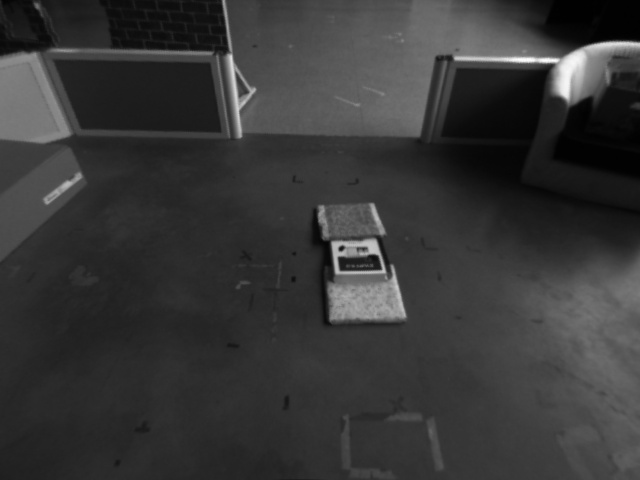
\includegraphics[scale=0.25]{Chap6-3D-Reconstruction/left0001}
\hspace{0.2cm}
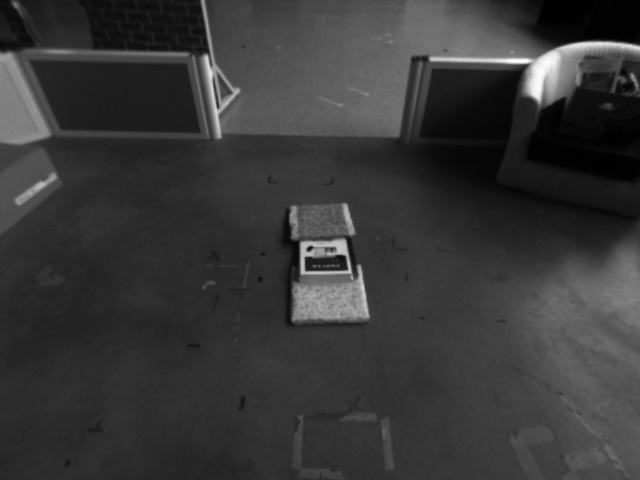
\includegraphics[scale=0.25]{Chap6-3D-Reconstruction/right0001}
\vspace{0.2cm}
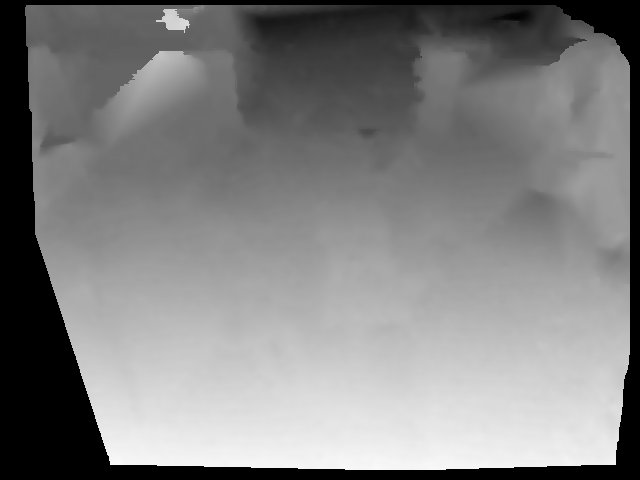
\includegraphics[scale=0.37]{Chap6-3D-Reconstruction/left0001_disp}
\vspace{0.2cm}
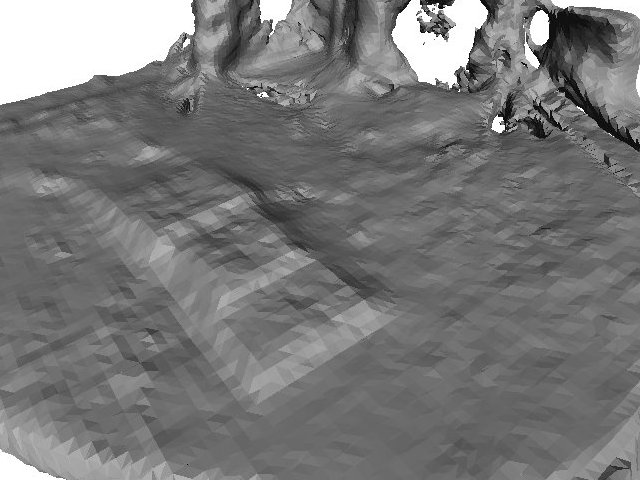
\includegraphics[scale=0.5]{Chap6-3D-Reconstruction/snapshot02}
\caption[]{From a pair of images of the scene in front of the robot
(left) we estimate a dense disparity map (middle) and from this
disparity map we estimate a dense surface integrating the previous
frames into the volumetric grid.}
\label{Fig:Reconstruction1}
\end{figure}


\begin{figure}[h]
\centering
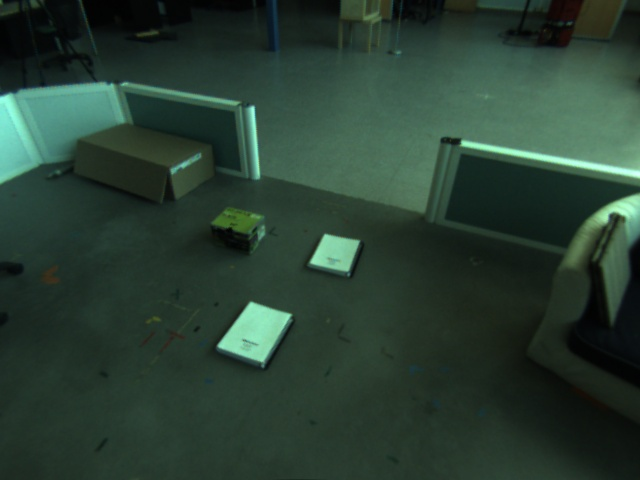
\includegraphics[scale=0.5]{Chap6-3D-Reconstruction/frame0005}
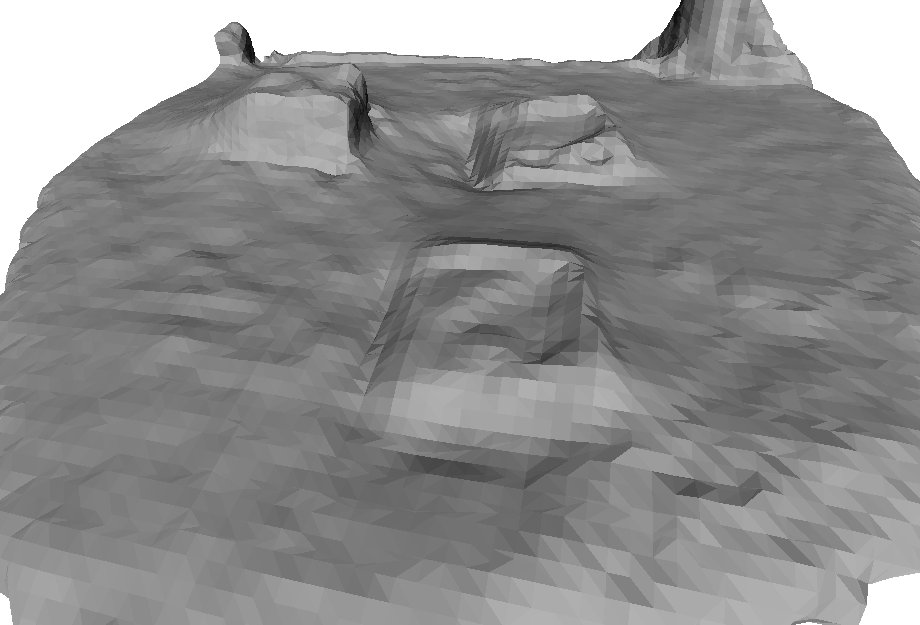
\includegraphics[scale=0.5]{Chap6-3D-Reconstruction/snapshot01}
\caption[]{Reconstruction of a scene of flat floor with small objects on it like books and boxes.}
\label{Fig:Reconstruction2}
\end{figure}

\begin{figure}[h]
\centering
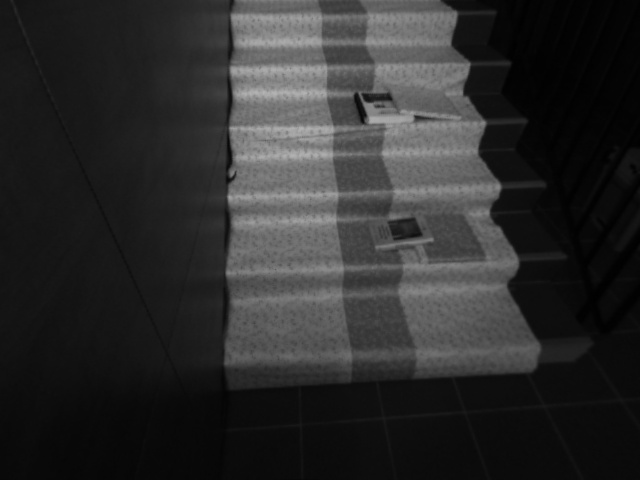
\includegraphics[scale=0.5]{Chap6-3D-Reconstruction/left0003}
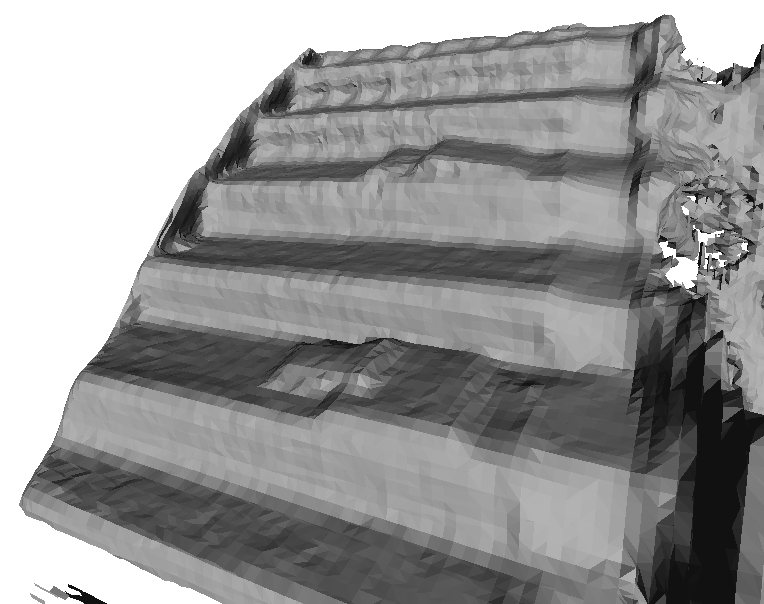
\includegraphics[scale=0.57]{Chap6-3D-Reconstruction/snapshot00}
\caption[]{Reconstruction of a stairs scene with some objects on it.}
\label{Fig:Reconstruction3}
\end{figure}

\begin{figure*}
\centering \footnotesize
\subfigure[\footnotesize \label{fig.w1}]{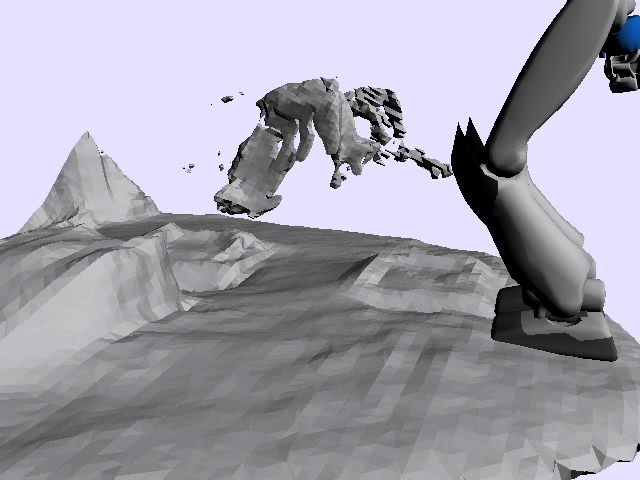
\includegraphics[width=0.35\linewidth ]{Chap6-3D-Reconstruction/robot-obstacle1.png}} ~  %\hfill
\subfigure[\footnotesize \label{fig.w2}]{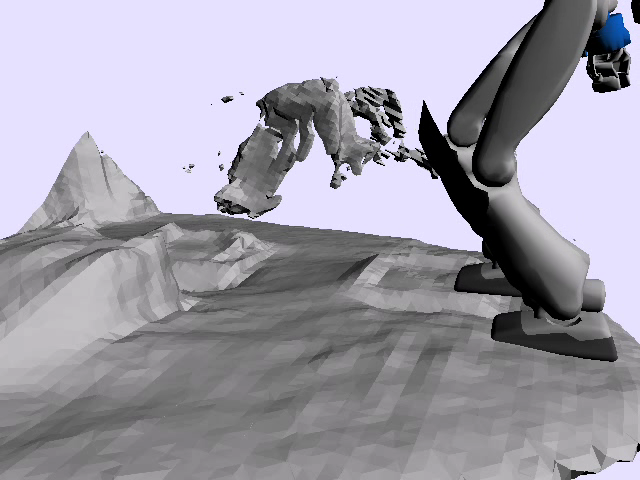
\includegraphics[width=0.35\linewidth]{Chap6-3D-Reconstruction/robot-obstacle2}} \\   %\hfill
\subfigure[\footnotesize \label{fig.w3}]{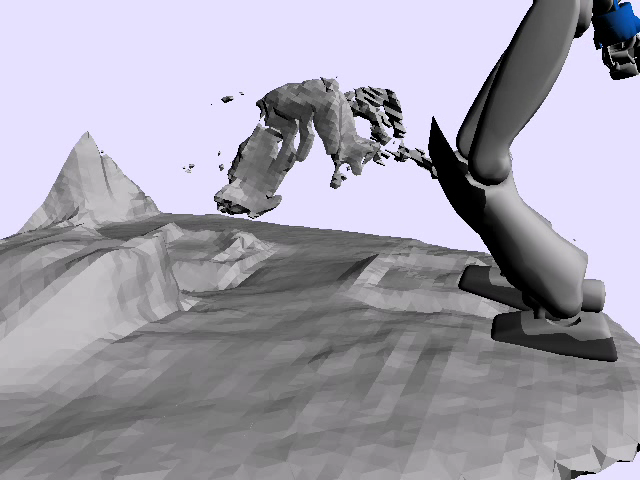
\includegraphics[width=0.35\linewidth]{Chap6-3D-Reconstruction/robot-obstacle3}}  ~ %\hfill
\subfigure[\footnotesize \label{fig.w3}]{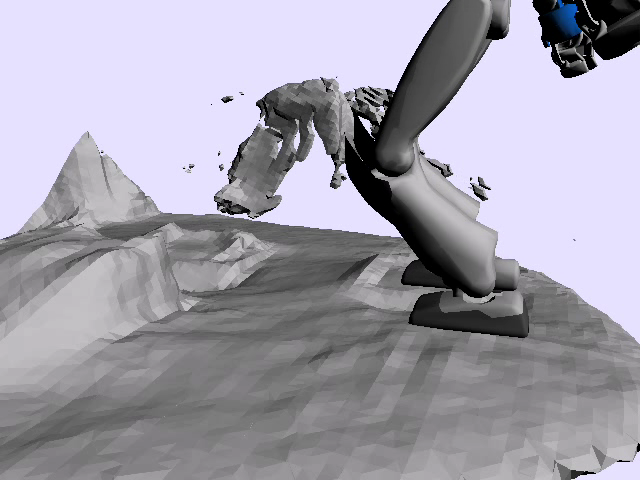
\includegraphics[width=0.35\linewidth]{Chap6-3D-Reconstruction/robot-obstacle4}} \\  %\hfill
\subfigure[\footnotesize \label{fig.w3}]{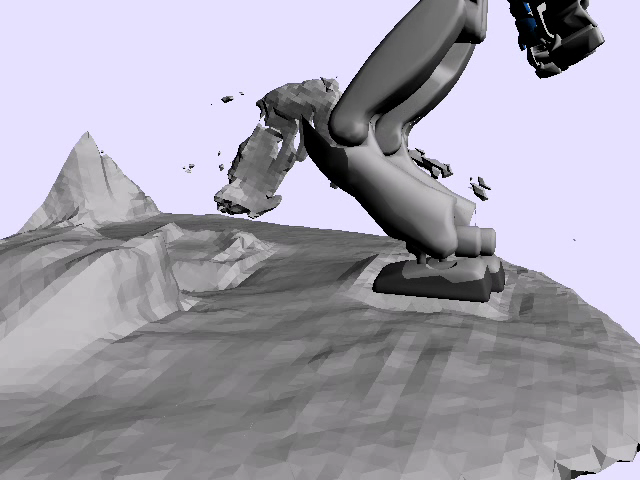
\includegraphics[width=0.35\linewidth]{Chap6-3D-Reconstruction/robot-obstacle5}} ~   %\hfill
\subfigure[\footnotesize \label{fig.w3}]{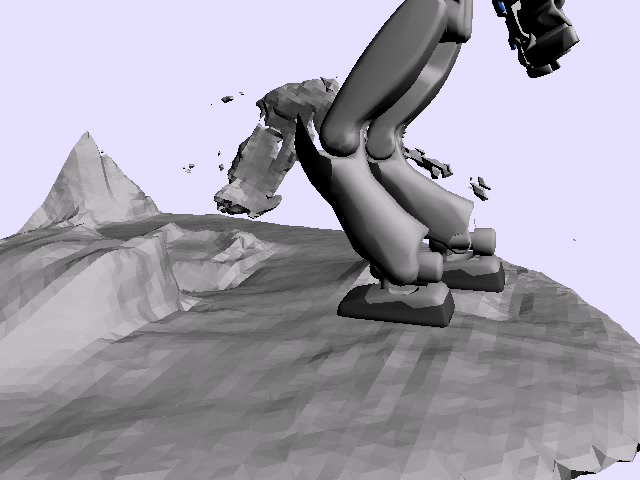
\includegraphics[width=0.35\linewidth]{Chap6-3D-Reconstruction/robot-obstacle6}}
\caption{HRP-2 walking on an obstacle.}
\label{fig.robot-walking-obstacle}
\end{figure*}

\section{Conclusion}

In this chapted we presented the connection of existing algorithms of eficient stereo matching and 3D reconstruction to be used in a more complex system to make the robot walk on rough terrain. This connection was done over ROS and tested succesfully with scenes of flat floor and stairs with small objects on them. The output of this algorithm provides a model of the world to a control system which implements a compliant walking scheme.

% Conclusions and Future Work
%\begin{savequote}[10cm]
%{\it ``You just can't differentiate between a robot and the very best of humans.''}
%\qauthor{Isaac Asimov}
%\end{savequote}

\chapter{Conclusions}
\label{Chap:Conclusions}

In this thesis, we tackled the problem of humanoid walking using visual information. Following the perception-decision-action paradigm, in this thesis we partially addressed all of them. A chain of improvements has been done since the ZMP Preview Control scheme was first introduced in \citep{Kajita2003}. We build on the work of prominent previous works and proposed new approaches to improve the humanoid walking.

\section{Contributions}

We presented a visual servoing scheme at the pattern generator level using Model Predictive Control. In the case of humanoid robots, visual servoing is a very useful approach for controlling precisely the robot position in contexts such as interactions with humans (to set the robot in front of a person), or to pre-position the robot before starting some manipulation tasks. The advantage of visual servoing is that the positioning task is defined relatively to a specific target. In any of the aforementioned applications, the higher-level navigation can be advantageously left to a planner, that would determine the sequence of landmarks, or human interactions, to reach consecutively. 

Since Visual Servoing is a local controller, we extended the scope of the pattern generation by directly introducing planning. Traditionally, planning was introduced at the pattern generator level using footprints. In our approach, we directly injected the motion primitives to the patterns generator using a velocity reference guided by a vector field.

In fact, these two paradigms are more complimentary than opposite: whereas planning may require high computational costs, but solve more complex problems of path finding, visual servoing is fast, by essence, but in general confined to local tasks that do not require high level reasoning, e.g. positioning the robot with respect to a given object.

Both contributions are based on Linear Model Predictive Control. However, due to the new optimization techniques and new computation performance, Nonlinear Model Predictive Control should be explored. This way we could use the whole-body motion instead of inverted pendulum simplification and moreover, deal with more accurate models.

Paralelly to the work of the pattern generation, we also presented an implementation of the connection of stereo matching and 3D reconstruction algorithms to be used by a walking control scheme. This reconstruction system was successfully tested on the HRP-2 robot and its output provides to a dynamic simulation of walking on rough terrain.

\section{Perspectives}

Our final goal is that the humanoid robots can achieve highly reactive motions in uncontrolled environments. Even if there has been impressive demonstrations of humanoid robots performing reactive motions based on perception, they are done in controlled environments. In current robotics, perception is one of the most important challenges.

In the control side, there already exists very suitable models of the humanoid locomotion and control. Those models are mainly stated as optimization problems. However, today's computers and algorithms can not solve in real time those complex models. Consequently, we rely in simplified but useful models to make the robots walk. Moreover, the introduction of torque controlled actuators can considerably improve the performance of humanoid motion.

Considering the current humanoid robotics development and challenges, we would like to continue contributing in humanoid locomotion based on vision. Always taking into account state of the art perception algorithms, optimization solvers and mathematical models of humanoid walking.



\bibliography{lathese}

\end{document}
